\captionsetup[subfigure]{font={normalfont, small}, skip=1pt, margin=7.2cm, singlelinecheck=false}

\section{Modelling Allele-Specific Copy Number Associated Changepoints}
CNAs in cancer have been extensively studied, however due to the complexity of cancer genomes, such as frequent deviations from diploidy and the presence of both tumour and non-tumour cells, many studies have been limited to reporting total CNAs across the genome. Total copy number profiling estimates the sum of the copy numbers of the two homologous chromosomes and as such only provides aggregate information. Determining the copy number landscape of each homologous chromosome, i.e. allele-specific copy number profiling, is important for the characterisation of certain types of genomic aberrations within tumour genomes, such as copy neutral loss of heterozygosity and the inference of their clonal history \citep{pmid20837533, pmid25477383}.  

In this chapter, measurements of allele-specific copy number profiling for the METABRIC cohort, using ASCAT \citep{pmid20837533}, is presented and a modelling framework is proposed for the detection and classification of changepoints in observed allele-specific copy number profiles, with a simulation study carried out to assess modelling approaches. These analyses aim to capture large scale changes in CNA state that occur on individual alleles, providing information on CNA events that may occur preferentially in certain genomic regions and whose downstream influence requires more investigation.  

\subsection{Allele-specific Copy Number Profiling using ASCAT}
A wide range of software is available facilitating measurement of allele-specific copy number, such as ASCAT \citep{pmid20837533}, Tumor Aberration Prediction Suite (TAPS) \citep{pmid22023820}, Parent-Specific-Copy-Number (PSCN) \citep{pmid21666266}, Patchwork \citep{pmid23531354}, Falcon \citep{pmid25477383}, Fraction and Allele-Specific Copy Number Estimates from Tumor Sequencing (FACETS) \citep{pmid27270079} and SPICE-pipeline \citep{CIANI2022183}. Giving consideration to software packages available for analysis of microarray data, specifically Affymetrix SNP6 data without matched normals, the type of output, and quality of documentation, ASCAT was deemed as most suitable for allele-specific copy number calling in this study. 

The ASCAT algorithm was applied first in \cite{pmid20837533}, to produce genome-wide allele-specific copy number profiles (ASCAT profiles) for 91/112 breast carcinoma samples genotyped on Illumina 109K SNP arrays. The paper reported that both the estimated percentages of aberrant cells and tumour ploidy were significantly different across the breast cancer subtypes, with the Luminal A subtype displaying the highest percentage of aberrant tumour cells and lowest ploidy. The frequency of gains and losses observed across the genome closely matched with previously reported patterns, but when stratifying by molecular subtype higher frequencies of gains and losses were observed in HER2 and Normal-like subtypes than reported previously. LOH was most frequently observed on chromosome arms 8p, 11q, 16q, and 17p, while copy number-neutral events were observed across the genome with a frequency of 20\% or higher. In addition, genomic regions with higher frequencies of losses were more likely to contain copy number-neutral events, this was particularly evident on chromosomes 1p, 2, 3, 4q, 9q, 15, and 19p.

As discussed in Section \ref{CARMA}, \cite{pmid32242091} utilised allele-specific copy number profiles, generated using ASCAT, to produce six metrics: AMP, DEL, STP, CRV, LOH, and ASM. The AMP, DEL, STP and CRV metrics were calculated using the sum of the allele-specific copy number, and all six metrics were combined into two prognostic indices, CPI and $\text{CPI}_\text{weighted}$. Notably, combining the metrics into a single index results in loss of valuable information, specifically the type of CNA observed and which allele the CNA is observed on. Other studies utilising ASCAT include \cite{pmid26205786, pmid27161491, pmid35705804, pmid36806386} and \cite{pmid36944408}. 

\subsection{Generation of Allele-specific Copy Number Profiles for METABRIC Patients}
To produce allele-specific copy number profiles from Affymetrix SNP 6.0 arrays, preprocessing using PennCNV (v1.0.5), a software tool to detect any form of copy number variation, is applied to generate signal intensity files, followed by ASCAT (v3.0.0), allele-specific copy number calling on these signal intensity files.

\subsubsection{PennCNV}
PennCNV \citep{pmid17921354} infers copy number calls for individual genotyped samples measured on genotyping arrays, such as Illumina and Affymetrix arrays, using a hidden Markov model, integrating multiple sources of information. 

PennCNV is applied to 1,992 Affymetrix SNP 6.0 CEL files, from the METABRIC study (study accession EGAS00000000083) \citep{pmid22522925, pmid26111507}, to generate signal intensity files. Two signal intensities of particular importance, as they serve as input variables to ASCAT, are Log R Ratio (LRR), the normalised measure of total signal intensity, and B-Allele Frequency (BAF), the normalised measure of relative signal intensity ratio of the B and A alleles. Generating the cross-marker normalised signal intensity data from these Affymetrix SNP 6.0 CEL files is a multi-step process that can be carried out using substep 1.1 to substep 1.4 of the PennCNV-Affy pipeline. These substeps include generating genotyping calls from the CEL files, allele-specific signal extraction, generating the canonical genotype clustering file and LRR and BAF calculation. When preprocessing the Affymetrix SNP 6.0 CEL files, for input into ASCAT, the PennCNV pipeline recommended by the creators of ASCAT, and subsequently applied here, contains three substeps, substeps 1.1, 1.2 and 1.4. More detailed information can be found in the comprehensive guide to using PennCNV-Affy at: \href{https://penncnv.openbioinformatics.org/en/latest/user-guide/affy/}{https://penncnv.openbioinformatics.org/en/latest/user-guide/affy/}.  

An example of the output obtained from the 3-substep PennCNV-Affy pipeline is provided in Table \ref{tab:PennCNV}, where rows display SNP/CN probes, and for each probe, columns provide the genomic location (chromosome and position) and the LRR and BAF values for samples. 

\begin{table}[H]
\caption[The first 15 rows of the output obtained from the PennCNV-Affy pipeline.]{The first 15 rows of the output obtained from the PennCNV-Affy pipeline. Only 9 columns are shown, corresponding to the first 3 METABRIC samples.}
\centering
\resizebox{\textwidth}{!}{\begin{tabular}{lrrrrrrrrrr}
\hline
Name & Chr & Position & MB.0000.LRR & MB.0000.BAF & MB.0002.LRR & MB.0002.BAF & MB.0005.LRR & MB.0005.BAF \\ 
\hline
SNP\_A-2131660 &     1 & 1156131 & 0.0784 & 0.0645 & 0.3256 & 0.4680 & -0.0204 & 0.6749 \\ 
SNP\_A-1967418 &     1 & 2234251 & -0.4757 & 0.8708 & -0.0664 & 0.9642 & 0.4691 & 0.9017 \\ 
SNP\_A-1969580 &     1 & 2329564 & -0.1603 & 0.9783 & 0.0210 & 0.8927 & -0.0135 & 0.8405 \\ 
SNP\_A-4263484 &     1 & 2553624 & -0.2693 & 0.9257 & -0.1307 & 0.1196 & -0.1347 & 0.0278 \\ 
SNP\_A-1978185 &     1 & 2936870 & 0.2567 & 0.0000 & 0.4048 & 0.0000 & 0.5406 & 0.0390 \\ 
SNP\_A-4264431 &     1 & 2951834 & -0.0046 & 0.9343 & 0.5220 & 0.4813 & -0.0062 & 0.8009 \\ 
SNP\_A-1980898 &     1 & 3095126 & 0.3309 & 1.0000 & 0.5433 & 1.0000 & 0.5810 & 1.0000 \\ 
SNP\_A-1983139 &     1 & 3165267 & 0.1509 & 0.0717 & 0.0452 & 0.0578 & -0.4310 & 0.0693 \\ 
SNP\_A-4265735 &     1 & 3302871 & 0.0285 & 0.0227 & 0.2208 & 0.5460 & -0.2972 & 0.2305 \\ 
SNP\_A-1995832 &     1 & 3705226 & 0.1941 & 0.5224 & 0.0320 & 0.5746 & 0.3774 & 0.6883 \\ 
SNP\_A-1995893 &     1 & 3720965 & 0.1675 & 0.5941 & 0.2923 & 0.9567 & 0.4228 & 0.7709 \\ 
SNP\_A-1997689 &     1 & 3763164 & -0.4370 & 0.9560 & -0.3390 & 0.8172 & -0.3035 & 0.8170 \\ 
SNP\_A-1997709 &     1 & 3763567 & -0.1209 & 0.0034 & -0.3431 & 0.0792 & -0.5607 & 0.0846 \\ 
SNP\_A-1997896 &     1 & 3766240 & 0.1209 & 0.0107 & 0.0167 & 0.0702 & 0.3122 & 0.6201 \\ 
SNP\_A-1997922 &     1 & 3766286 & -0.0838 & 0.0018 & -0.0365 & 0.9161 & -0.5464 & 0.0287 \\ 
\hline
\end{tabular}}
\label{tab:PennCNV}
\end{table}

\subsubsection{ASCAT}
ASCAT, applicable to Illumina SNP arrays, Affymetrix SNP arrays and high-throughput sequencing data, is used to derive allele-specific copy number profiles of tumour cells, accounting for non-aberrant cell admixture and aneuploidy. ASCAT produces profiles that map the distribution of allele-specific gains and losses, revealing LOH and copy number-neutral events, across the genome \citep{pmid20837533}. ASCAT is available as an R package and can be found on GitHub at: \href{https://github.com/VanLoo-lab/ascat}{https://github.com/VanLoo-lab/ascat}.  

ASCAT can be run in a number of different ways such as with or without matched normals or with or without a logR correction step. The ASCAT pipeline implemented here is for Affymetrix Genome-Wide Human SNP Array 6.0 CEL files, without matched normals, with a logR correction (GC content and replication timing) and where all samples are from females, adapted from the \texttt{ASCAT\_fromCELfiles.R} script available on GitHub. Implementing this pipeline 1,984 ASCAT profiles were generated from 1,992 samples. 

Outputs obtained from the ASCAT pipeline include a dataframe containing the copy number segments of each sample, an example of which is provided in Table \ref{tab:ASCAT}, allele-specific copy number profiles for each sample (Figure \ref{fig:s1}), together with quality control metrics from ASCAT profiles including information on the purity and ploidy of each sample. Table \ref{tab:PennCNV} shows the copy numbers for each allele, nMajor and nMinor, which take on values 0 (indicating deletion), 1 (indicating normal copy number of allele), or any positive whole number greater than 1 (indicating increasing levels of amplifications). In Figure \ref{fig:s1} the Minor and Major allele are coloured blue and red, respectively. The allele-specific copy number profile illustrated in Figure \ref{fig:s1}A, observed for sample MB.0000, provides an example of a tumour sample that has very little GI, as very few chromosomes contain CNAs. Samples such as this are labelled as “non-aberrant”. The allele-specific copy number profile observed for sample MB.0025 provides an example of a tumour sample with moderate GI (Figure \ref{fig:s1}B). In the observed sample, some chromosomes contain no CNAs (chromosomes 4, 9 and 13), while others contain numerous CNAs (chromosomes 1, 3, 17). The amplification and deletion observed separately on chromosome 3 are examples of genomic aberrations that would not be detected in total CNA data, as the total copy number is 2. The allele-specific copy number profile observed for sample MB.0062 provides an example of a tumour sample with widespread GI, the majority of chromosomes contain at least one CNA and there are high levels of fluctuations between the CNA states (Figure \ref{fig:s1}C).

\begin{figure}[!h]
\vspace{0.3cm}
\centering
\subfloat[]{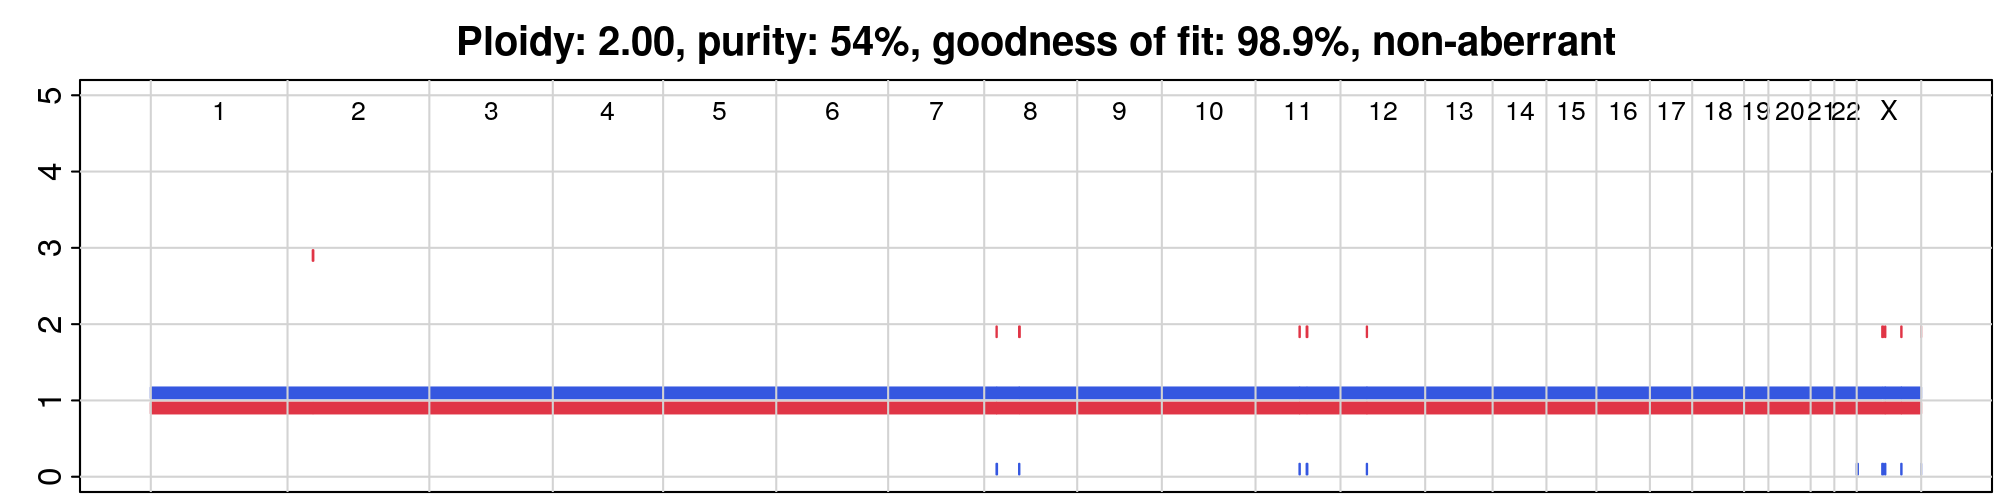
\includegraphics[width = 1\textwidth]{../figures/Chapter_5/MB.0000.ASCATprofile.png}}
\vspace{0.8cm}
\subfloat[]{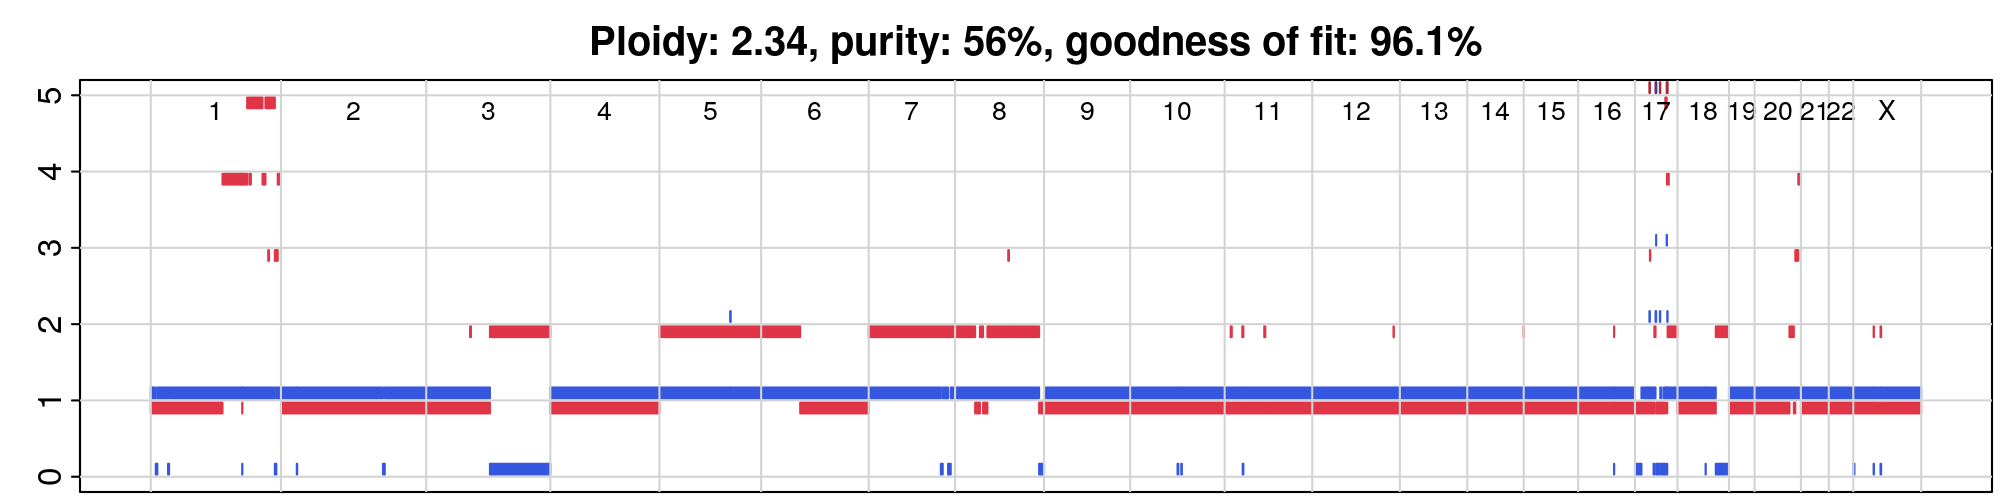
\includegraphics[width = 1\textwidth]{../figures/Chapter_5/MB.0025.ASCATprofile.png}}
\vspace{0.8cm}
\subfloat[]{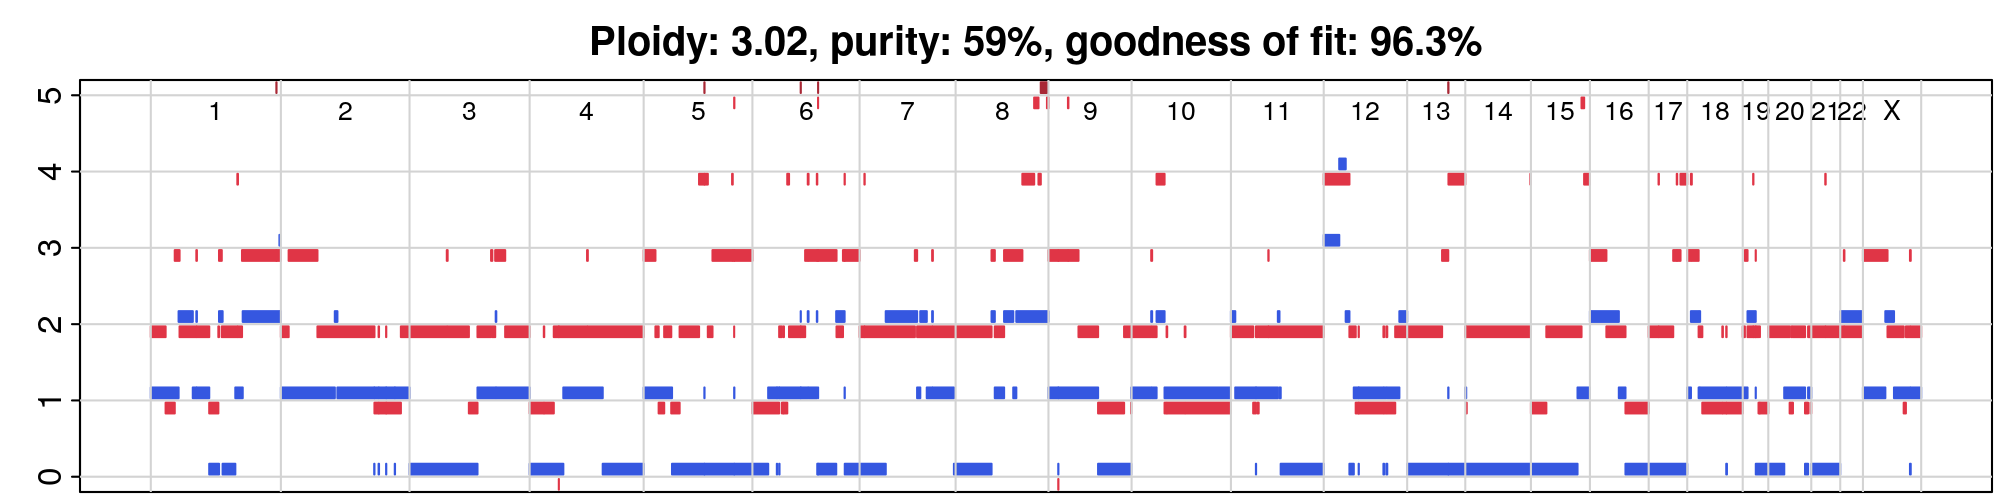
\includegraphics[width = 1\textwidth]{../figures/Chapter_5/MB.0062.ASCATprofile.png}}
\caption[Allele-specific copy number profiles of three METABRIC samples.]{Allele-specific copy number profiles of (A) sample MB.0000, (B) sample MB.0025 and (C) sample MB.0062. Ploidy is defined as the amount of DNA relative to a haploid genome and purity is defined as the percentage of tumour cells. These ploidy and purity estimates are generated by creating a grid of possible values and evaluating the goodness-of-fit for both parameters \citep{pmid20837533}.}
\label{fig:s1}
\end{figure}

\subsubsection{Reformatting ASCAT Output for Downstream Analysis}
It is useful to recode the copy numbers so they correspond to deletion, neutral and amplification states. In this case any probe that has a copy number greater than 2 will be assigned a 2, resulting in only three possible copy number values, 0, 1  and 2. Table \ref{tab:ASCAT} shows that after reformatting, the copy number of each allele, nMajorRF and nMinorRF, is bound in the range [0-2]. 

\begin{table}[!ht]
\centering
\caption[First 20 rows of the ASCAT segments file containing the allele-specific copy number calls for each sample.]{The first 20 rows of the ASCAT segments file containing the allele-specific copy number calls for each sample. nMajor and nMinor refer to the copy numbers of the Major and Minor allele, while nMajorRF and nMinorRF refer to the reformatted copy numbers of the Major and Minor allele.}
\resizebox{0.98\textwidth}{!}{\begin{tabular}{rlrrrrrrr}
\hline
sample & chr & startpos & endpos & nMajor & nMinor & nMajorRF & nMinorRF \\ 
\hline
MB.0000 & 1 & 61735 & 152555527 &     1 &     1 &     1 &     1 \\ 
MB.0000 & 1 & 152555706 & 152586540 &     0 &     0 &     0 &     0 \\
MB.0000 & 1 & 152586576 & 152761923 &     1 &     1 &     1 &     1 \\
MB.0000 & 1 & 152761939 & 152768700 &     0 &     0 &     0 &     0 \\
MB.0000 & 1 & 152773905 & 249224388 &     1 &     1 &     1 &     1 \\
MB.0000 & 2 & 12784 & 32630548 &     1 &     1  &     1 &     1 \\ 
MB.0000 & 2 & 32635284 & 33331778 &     3 &     1  &     2 &     1 \\ 
MB.0000 & 2 & 33333871 & 243089456 &     1 &     1  &     1 &     1 \\ 
MB.0000 & 3 & 60345 & 197896118 &     1 &     1  &     1 &     1 \\ 
MB.0000 & 4 & 12281 & 191027923 &     1 &     1  &     1 &     1 \\ 
MB.0000 & 5 & 15532 & 180790320 &     1 &     1 &     1 &     1 \\ 
MB.0000 & 6 & 149661 & 171051005 &     1 &     1  &     1 &     1 \\ 
MB.0000 & 7 & 43259 & 159127004 &     1 &     1 &     1 &     1 \\ 
MB.0000 & 8 & 31254 & 10555654 &     1 &     1 &   1 &     1 \\ 
MB.0000 & 8 & 10555762 & 11310012 &     2 &     0 &     2 &     0 \\ 
MB.0000 & 8 & 11322997 & 11701198 &     1 &     0 &     1 &     0 \\ 
MB.0000 & 8 & 11701253 & 41811521 &     1 &     1 &     1 &     1 \\ 
MB.0000 & 8 & 41811769 & 49326113 &     2 &     0 &     2 &     0 \\ 
MB.0000 & 8 & 49328524 & 51634513 &     2 &     1 &     2 &     1 \\ 
MB.0000 & 8 & 51634751 & 146298155 &     1 &     1 &     1 &     1 \\ 
\hline
\end{tabular}}
\label{tab:ASCAT}
\end{table}

\subsection{Classification of Changepoints in Allele-specific CNA Profiles}
Our aim here is to model the allele-specific copy number profile across the genome by modelling features of common changes in the profile by detection of changepoints, also known as breakpoints, in the allele-specific CNA profiles. We define a copy number changepoint as a point along a chromosome, corresponding to an individual allele, where there is a change in copy number, i.e. if there is a copy number change from 2 to 0, there exists a point along that chromosome where the change has occurred (Figure \ref{fig:MockASCAT_1}). Figure \ref{fig:MockASCAT_1}, an annotated allele-specific profile, displays the different copy number states, Neutral (N) for a copy number of 1, Deletion (D) for a copy number of 0 and Amplification (A) for a copy number of 2. This figure highlights a copy number changepoint (CP) where the CNA state has gone from A to D. Based on the copy number either side of the changepoint we categorise each changepoint as either Neut/Amp (1 to 2), Neut/Del (1 to 0), Amp/Neut (2 to 1), Del/Neut (0 to 1), Amp/Del (2 to 0) or Del/Amp (0 to 2). Where no changepoint occurs, the category is labelled NoChangepoint. The detection of changepoints is based on length of the alteration segment to the left of the changepoint ($TS$) and the length of the alteration segment to the right of the changepoint ($TE$). For each copy number changepoint, for each sample, we record the changepoint location (chromosome, genomic position and allele), the $TS$ and $TE$ lengths, and the assigned category (Table \ref{ReformattedData}). In the case where there is a gap between the segments, and as such between the copy number changes, the midpoint of the segment is used as the genomic position of the changepoint. Summary statistics of the $TS$ and $TE$ lengths for each category in the ASCAT data are shown in Tables \ref{tbl:excel-table1} and \ref{tbl:excel-table2}. 

\begin{figure}[!ht]
\center
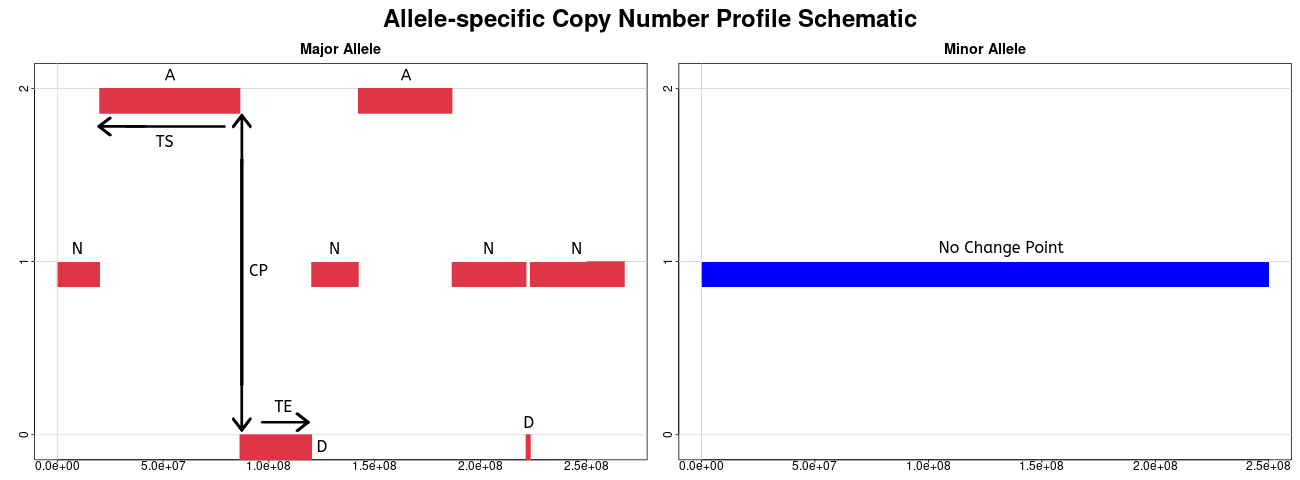
\includegraphics[width = 1\textwidth]{../figures/Chapter_5/Annotated_ASCAT_Profile.png}
\caption[Copy number profiles of the Major and Minor alleles denoting changepoints, alteration states and $TS$/$TE$ lengths.]{Copy number profiles of the Major and Minor alleles denoting changepoints, alteration states and $TS$/$TE$ lengths.}
\label{fig:MockASCAT_1}
\end{figure}

Further examples of simulated allele-specific copy number profiles are provided in Figure \ref{fig:MockASCAT}. Profile A illustrates both the Major and Minor allele having a copy number of 1 across the observed region, both alleles are categorised as NoChangepoint. Profile B illustrates the Major allele having an amplified segment flanked by two neutral segments, categorised as Neut/Amp and Amp/Neut, and the Minor allele categorised as NoChangepoint. Profile C illustrates the Major allele having an amplified segment followed by a deleted segment, what we define as an Amp/Del flashpoint pattern, flanked by two neutral segments, categorised as Neut/Amp, Amp/Del and Del/Neut, and the Minor allele categorised as NoChangepoint. Profile D illustrates the Major allele displaying an Amp/Del flashpoint pattern, flanked by two neutral segments, and the Minor allele displaying an oscillating pattern of deleted and neutral segments, categorised as Neut/Del and Del/Neut. 

\begin{table}[H]
\vspace{-0.3cm}
\centering
\caption[First 15 rows of the reformatted ASCAT segments file containing the allele-specific copy number calls for each sample.]{First 15 rows of the reformatted ASCAT segments file containing the allele-specific copy number calls for each sample. $TS$ and $TE$ displayed in bases.}
\begin{tabular}{rlrrrrr}
  \hline
 Sample & Chr & Changepoint & Allele & TS & TE & Category \\ 
  \hline
MB.0000 & 1 & 152555616.5 & Major & 0 & 30941.5 & Neut/Del \\ 
MB.0000 & 1 & 152586558 & Major & 30941.5 & 0 & Del/Neut  \\ 
MB.0000 & 1 & 152761931 & Major & 0 & 9371.5 & Neut/Del \\ 
MB.0000 & 1 & 152771302.5 & Major & 9371.5 & 0 & Del/Neut \\ 
MB.0000 & 2 & 32632916 & Major & 0 & 699908.5 & Neut/Amp \\ 
MB.0000 & 2 & 33332824.5 & Major & 699908.5 & 0 & Amp/Neut  \\ 
MB.0000 & 3 &  & Major & 0 & 0 & NoChangepoint \\ 
MB.0000 & 4 &  & Major & 0 & 0 & NoChangepoint  \\ 
MB.0000 & 5 &  & Major & 0 & 0 & NoChangepoint  \\ 
 MB.0000 & 6 &  & Major & 0 & 0 & NoChangepoint  \\ 
 MB.0000 & 7 &  & Major & 0 & 0 & NoChangepoint  \\ 
 MB.0000 & 8 & 10555708 & Major & 0 & 760796.5 & Neut/Amp  \\ 
 MB.0000 & 8 & 11316504.5 & Major & 760796.5 & 0 & Amp/Neut  \\ 
 MB.0000 & 8 & 41811645 & Major & 0 & 9822987 & Neut/Amp \\ 
 MB.0000 & 8 & 51634632 & Major & 9822987 & 0 & Amp/Neut \\ 
   \hline
\end{tabular}
\label{ReformattedData}
\end{table}
 
\begin{table}[H]
\vspace{0.2cm}
  \caption[Summary statistics of the ASCAT segment kilobase lengths where the length of the neutral segments are set to 0.]{Summary statistics of the ASCAT segment kilobase lengths where the length of the neutral segments are set to 0. n refers to the number of changepoints.}
  \label{tbl:excel-table1}
  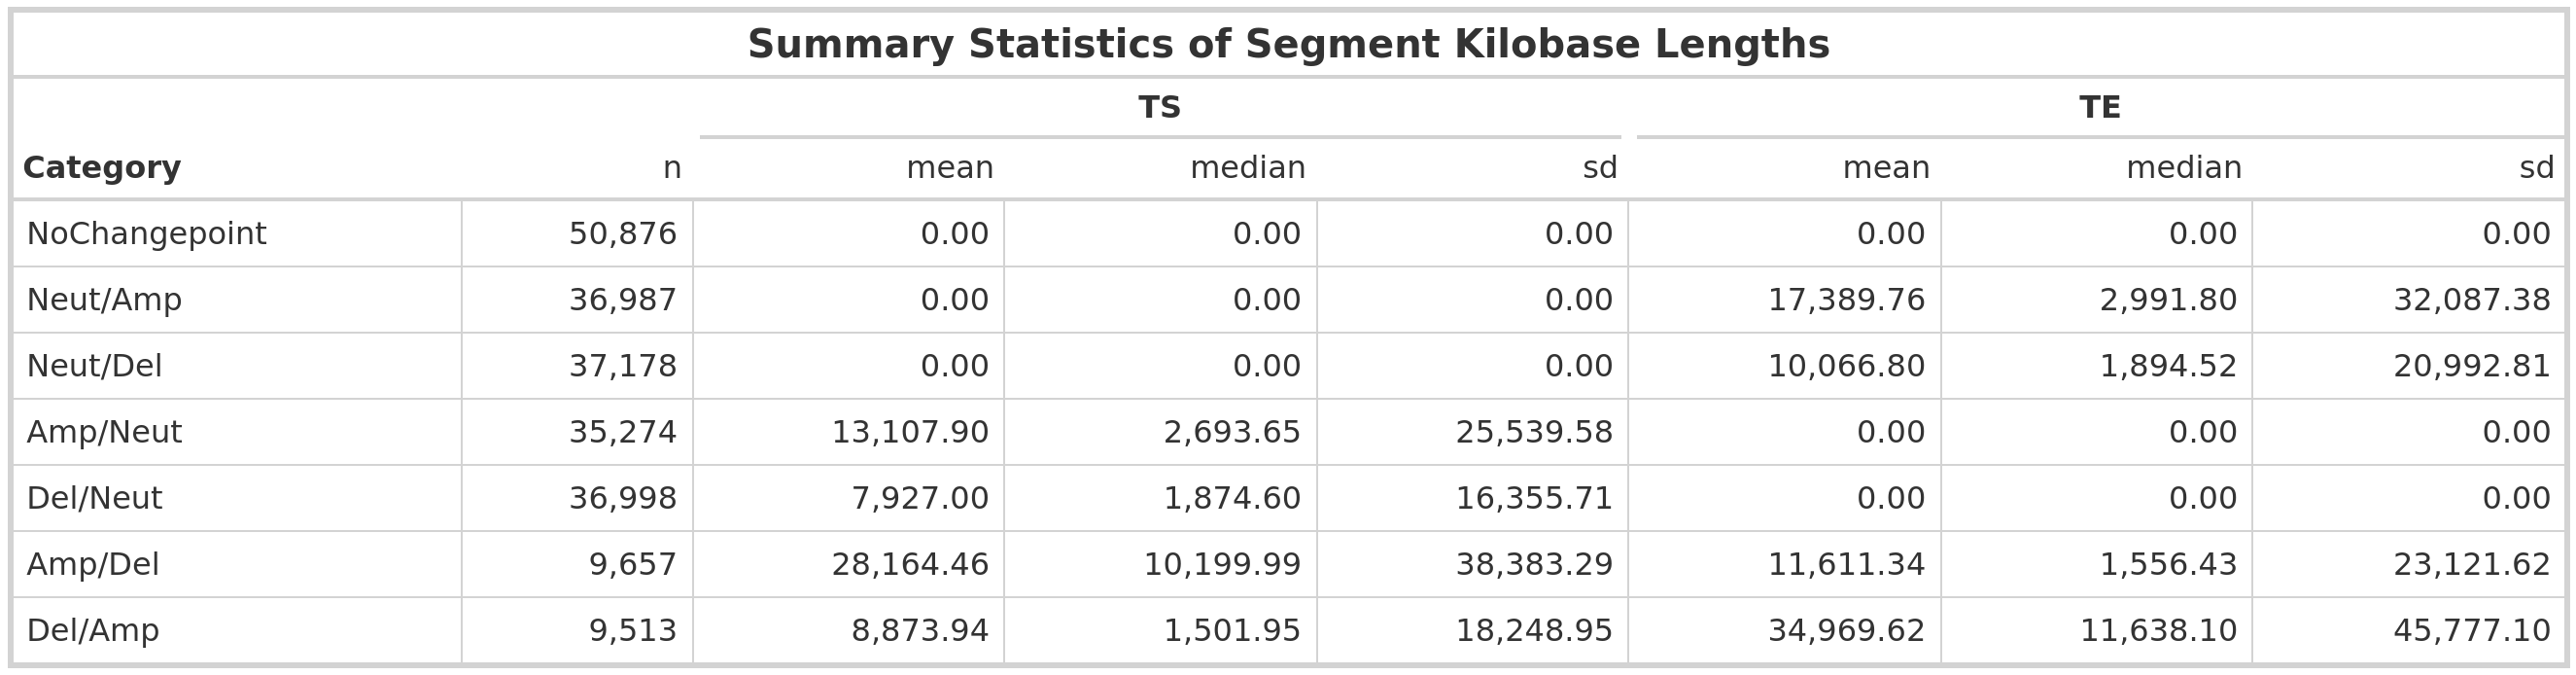
\includegraphics[width=\linewidth]{../tables/Chapter_5/ASCAT_Summary_Table_All_Zero.png}
\end{table}

\begin{table}[H]
  \caption[Summary statistics of the ASCAT segment kilobase lengths where the length of the neutral segments are recorded as greater than 0.]{Summary statistics of the ASCAT segment kilobase lengths where the length of the neutral segments are recorded as greater than 0. n refers to the number of changepoints.}
  \label{tbl:excel-table2}
  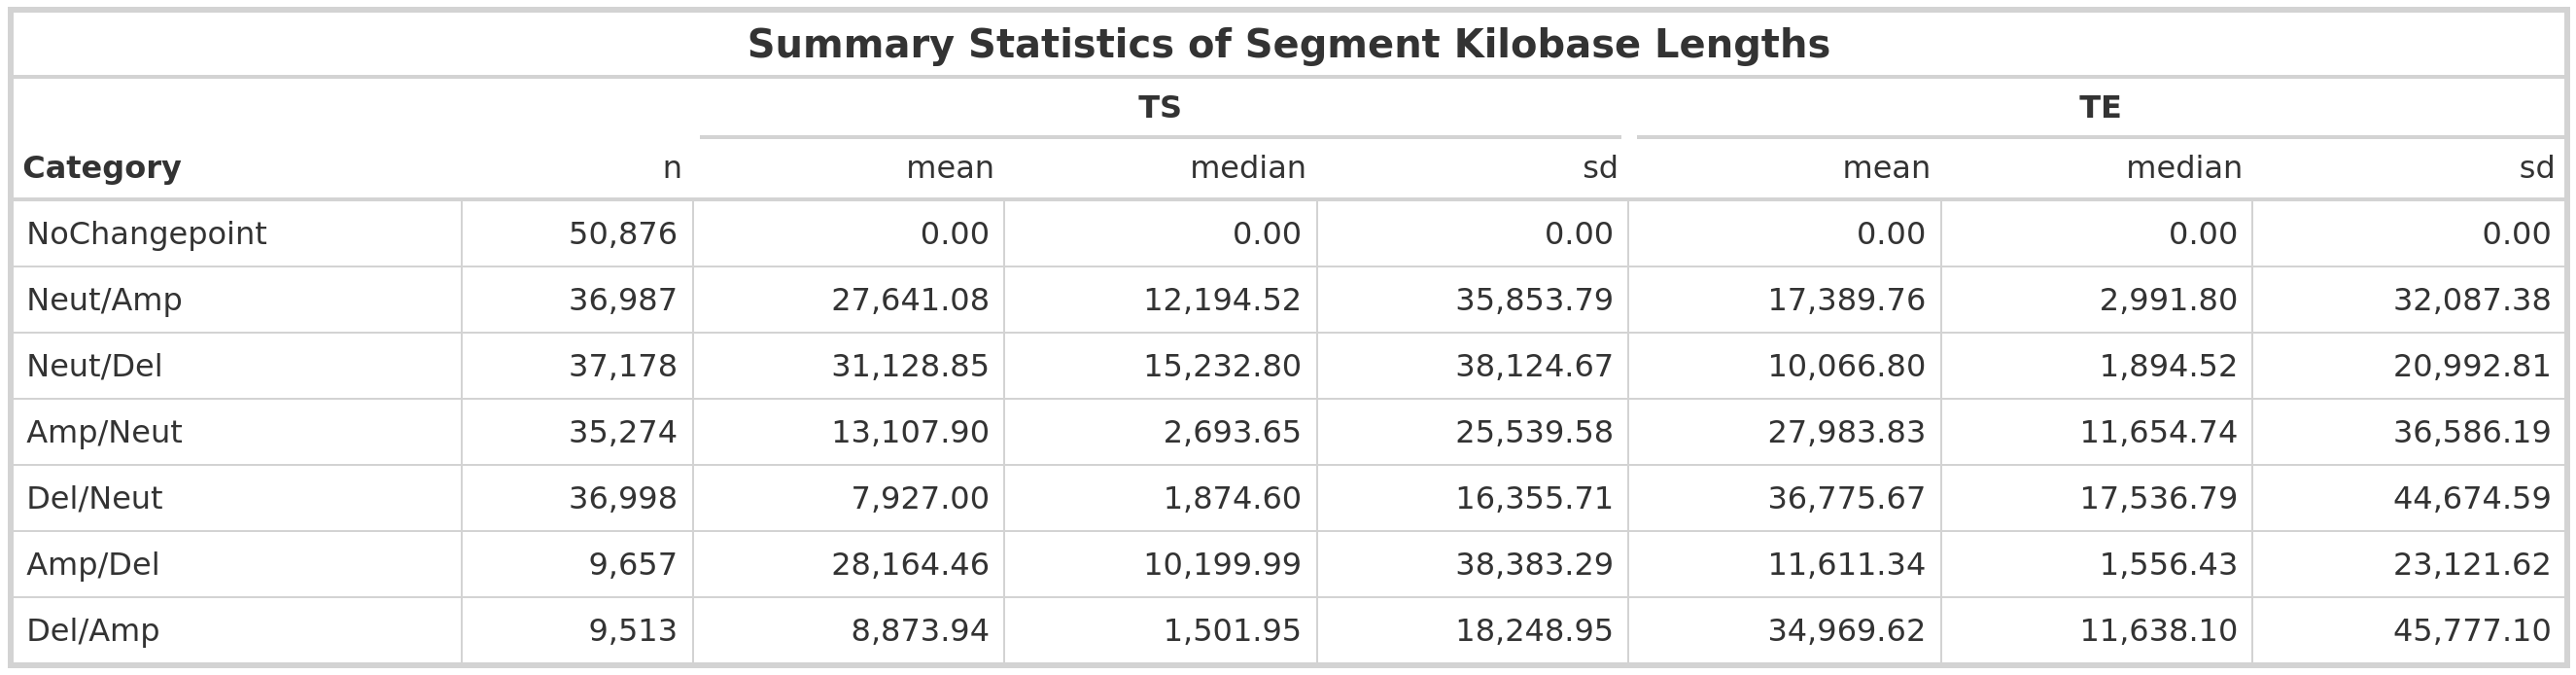
\includegraphics[width=\linewidth]{../tables/Chapter_5/ASCAT_Summary_Table_All_NoZero.png}
\end{table}

\begin{figure}[!ht]
\center
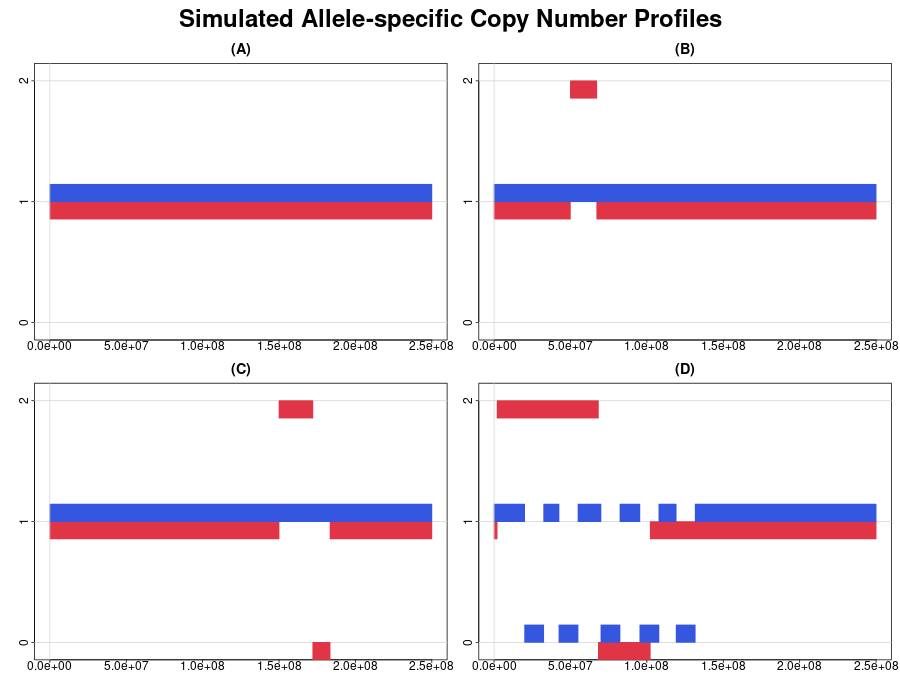
\includegraphics[width = 0.88\textwidth]{../figures/Chapter_5/Example_ASCAT_Scen.png}
\caption[Simulated allele-specific copy number profiles]{Simulated allele-specific copy number profiles. Minor allele in blue and Major allele in red.}
\label{fig:MockASCAT}
\end{figure}
\FloatBarrier 

\subsection{Proposed Models for Changepoints in Allele-specific CNA Profiles} \label{models}
Our modelling approach has two aims: to enable the detection of changepoints and to model the features of changepoints across the observed allele-specific CNA profile, with two alleles labelled as Major and Minor, for all observed patients. 

Given a specified interval of observation $d$ where a changepoint is observed in an allele, the type of changepoint (Category) is recorded as one of six categories: Neut/Amp, Neut/Del, Amp/Neut, Del/Neut, Amp/Del and Del/Amp. The features of the observed changepoint are recorded as two continuous response variables $TS$ and $TE$, representing the lengths of the segments to the left ($TS$) and to the right ($TE$) of the changepoint. These lengths are recorded irrespective of the interval boundaries, i.e. lengths $>d$ may be observed. 

Where the category contains a Neutral flanking segment (Neut/Amp, Neut/Del, Amp/Neut, Del/Neut) this length can be recorded or set to 0. For the specified interval of observation, if no changepoints of any kind are observed in the interval, the category NoChangepoint can be recorded, within which $TS=TE=0$.

\subsubsection{Allele-Independent (AI) Models} \label{Model1}
Treating the information from both alleles as independent, the following models the average $TS$ length feature, the first response variable, given the type of changepoint: 

\begin{equation}
\begin{aligned}
TS_{ij}&=\beta_0+ \beta_1 NeutAmp_{ij} + \beta_2NeutDel_{ij}+ \beta_3AmpNeut_{ij} +  \\
       & \mathrel{\phantom{=}} \beta_4DelNeut_{ij}+ \beta_5AmpDel_{ij} + \beta_6DelAmp_{ij} + \epsilon_{ij}\\
\end{aligned}
\label{Eq1}
\end{equation}

For an observed interval $d$, where there are $n_1$ number of changepoints on the Major allele for individual $i$ and $n_2$ number of changepoints on the Minor allele for individual $i$, the information on both alleles for an individual are included as independent observations, so that $j\in [1: (n_1+n_2)]$ for individual $i$.

Similarly, for each of the changepoints ${j}$, the average $TE$ length feature, the second response variable, for each type of changepoint is specified as:

\begin{equation}
\begin{aligned}
TE_{ij}&=\beta_0+ \beta_1 NeutAmp_{ij} + \beta_2NeutDel_{ij}+ \beta_3AmpNeut_{ij} +  \\
       & \mathrel{\phantom{=}} \beta_4DelNeut_{ij}+ \beta_5AmpDel_{ij} + \beta_6DelAmp_{ij} + \epsilon_{ij}\\
\end{aligned}
\label{Eq1.1}
\end{equation}

In the above intercept model specification, where regions containing no changepoints are observed in the observation range for individual $i$, and the NoChangepoint observations are included in the data, the intercept, $\beta_0$, serves as the baseline category (NoChangepoint). Since the mean $TS$ and $TE$ lengths for the baseline group, NoChangepoint, are equal to 0, the coefficients of each of the six changepoint categories correspond directly to the mean response lengths for those categories. 

Alternatively, where the NoChangepoint observations are excluded from the observed dataset, the intercept is removed from the model to maintain this interpretation and the models are specified as: 

\begin{equation}
\begin{aligned}
TS_{ij}&=\beta_1 NeutAmp_{ij} + \beta_2NeutDel_{ij}+ \beta_3AmpNeut_{ij} +  \\
       & \mathrel{\phantom{=}} \beta_4DelNeut_{ij}+ \beta_5AmpDel_{ij} + \beta_6DelAmp_{ij} + \epsilon_{ij}\\
\end{aligned}
\label{Eq2}
\end{equation}

\begin{equation}
\begin{aligned}
TE_{ij}&= \beta_1 NeutAmp_{ij} + \beta_2NeutDel_{ij}+ \beta_3AmpNeut_{ij} +  \\
       & \mathrel{\phantom{=}} \beta_4DelNeut_{ij}+ \beta_5AmpDel_{ij} + \beta_6DelAmp_{ij} + \epsilon_{ij}\\
\end{aligned}
\label{Eq22}
\end{equation}

We refer to this as the Allele-Independent Non-Intercept Model (AINIM) and the former as the Allele-Independent Intercept Model (AIIM). 

For both AINIM and AIIM, $TS$ and $TE$ are also jointly modelled using the multivariate response vector, $Y_{ij}=(TS_{ij},\:TE_{ij})$, which captures the covariance structure between the two response variables, $\Sigma = \sigma^2 \textit{I}$. 

The assumptions of the proposed linear models include linearity, normality for any fixed value of the predictor variable, homoscedasticity, and independence. 

These models were fit using two R functions, \texttt{lm()} from the stats package \citep{stats} and \texttt{MCMCglmm()} from the MCMCglmm package \citep{MCMCglmm}. While the \texttt{lm()} function can be used to fit basic linear regression models, \texttt{MCMCglmm()} (with default priors) should produce similar results but provides more flexibility. 

\paragraph{Illustration of Allele-Independent (AI) Model}
\hfill
\newline

\noindent The AI Models, AIIM (Equations \ref{Eq1} and \ref{Eq1.1}) and AINIM (Equations \ref{Eq2} and \ref{Eq22}), are fitted to a simulated dataset using the two response variables in a univariate approach and multivariate approach. The simulated dataset is simulated as n = 20 patient tumour samples, of which 20\% have allele-specific copy number profile A, 40\% have allele-specific copy number profile C and 40\% have allele-specific copy number profile D. As a result, samples 1 to 4 have profile A, samples 5 to 12 have profile C, and samples 13 to 20 have profile D (Table \ref{tab:Model_Example}). For all samples, the lengths of the neutral segments, in addition to the lengths of the amplified and deleted segments, are simulated from a truncated Normal distribution with parameters specified in Table \ref{tab:Param_Small}. 

\begin{table}[!htb]
\center
\caption[Parameters of truncated Normal distributions used to simulate segment length and properties of simulated data.]{Parameters of truncated Normal distributions used to simulate segment length and properties of simulated data. a and b correspond to the lower and upper bound.}
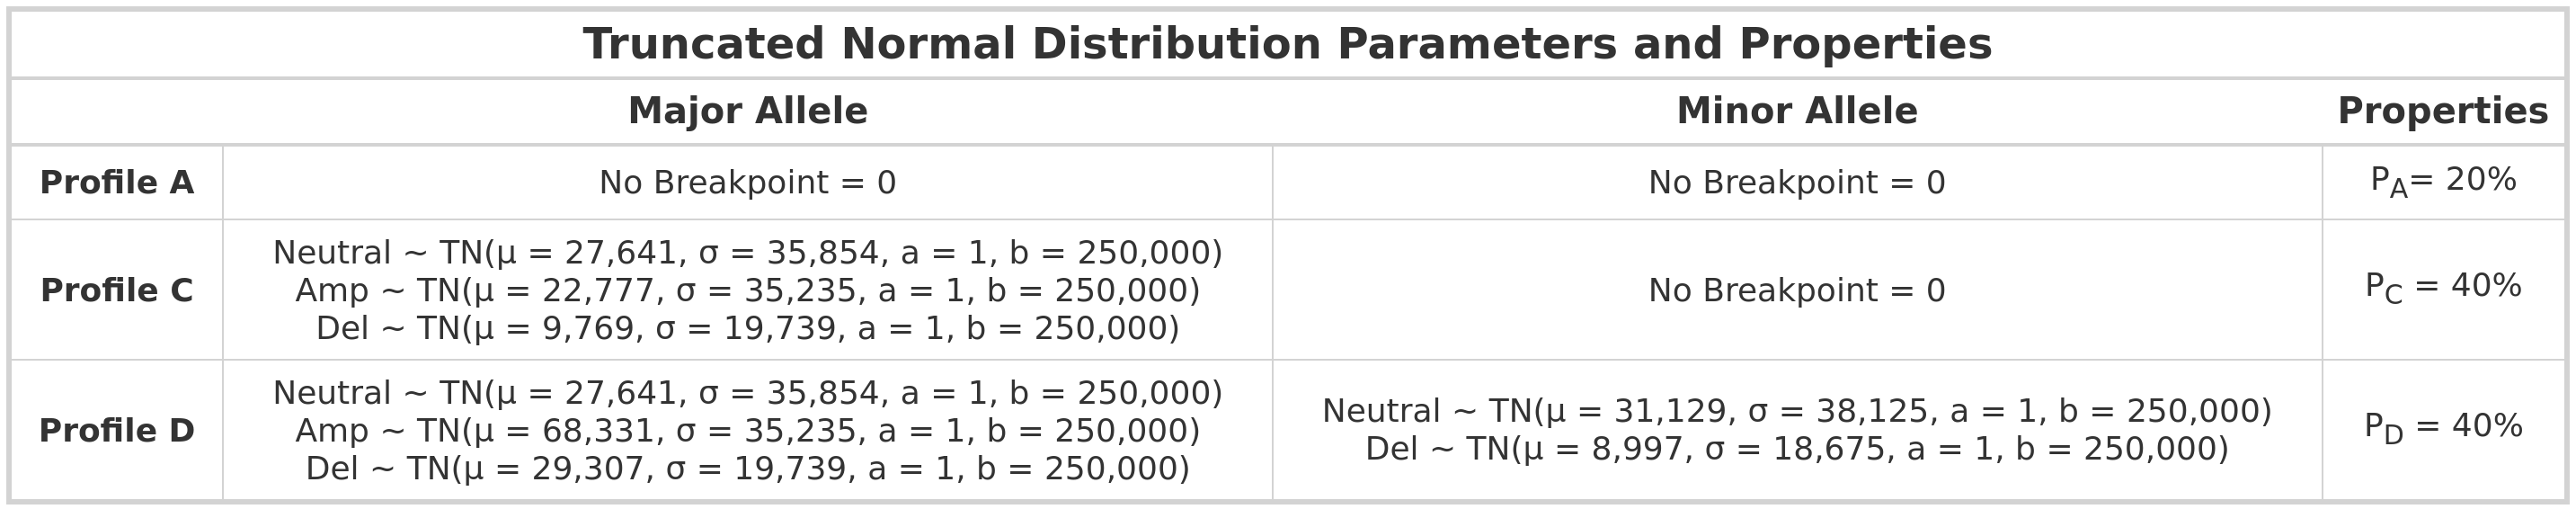
\includegraphics[width = 1\textwidth]{../tables/Chapter_5/TN_Distribution_2.png}
\label{tab:Param_Small}
\end{table}

Table \ref{tab:Model_Example}A provides a snapshot of simulated data values where lengths of neutral segments are set to 0, while Table \ref{tab:Model_Example}B provides information on simulated data values where lengths of neutral segments are retained as greater than 0. Table \ref{tab:three_tables} provides summary statistics for the full simulated datasets. From these tables we can see the sample size, mean, median and standard deviation of the $TS$ and $TE$ variables corresponding to the different categories of changepoints. These tables highlight that each simulated sample contributes at least two changepoint observations to the dataset and that the number of changepoints observed is dependent on the cumulative length of the region. 

\vfill 
\begin{table}[!h]
    \caption[Structure of single simulated dataset.]{Structure of single simulated dataset. Simulated sample 1, sample 5 and sample 13, displaying the possible allele-specific copy number profiles, are shown.}
    \label{tbl:scen3_structure}
     \begin{subtable}[t]{.49\textwidth}
      \caption{Dataset where neutral segment length recorded as length 0.}
      \centering
      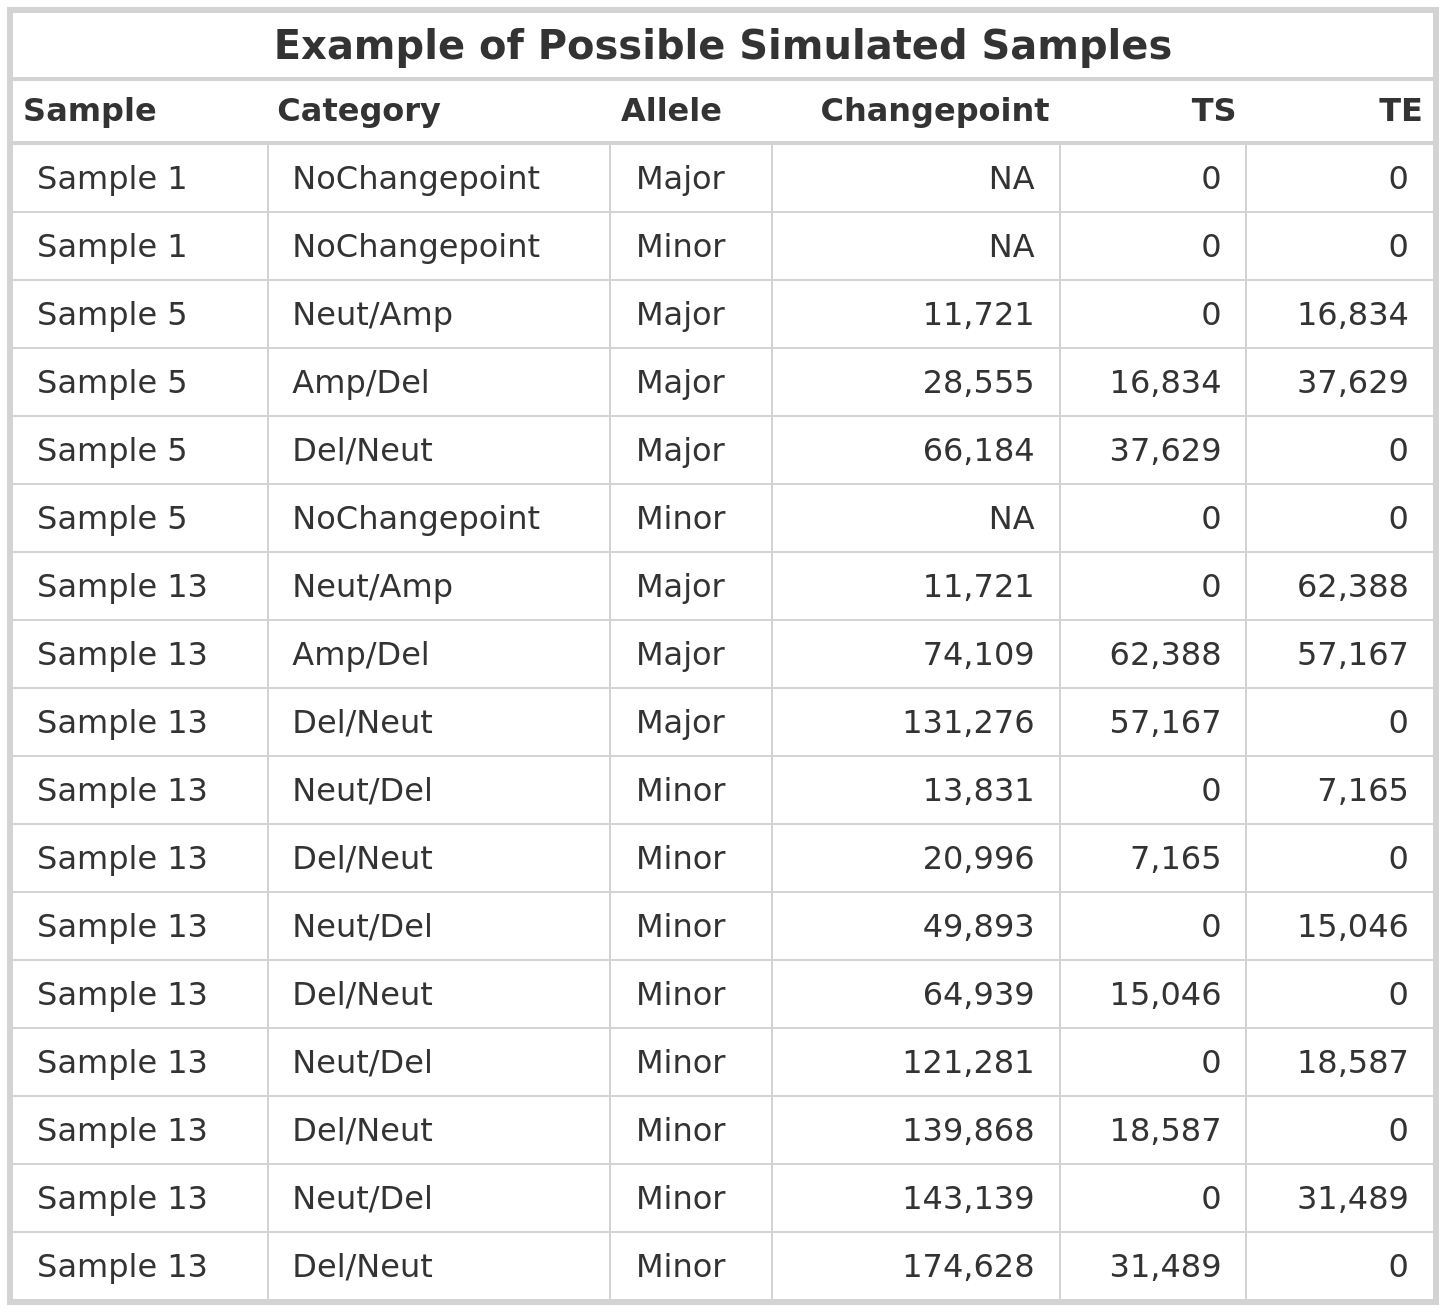
\includegraphics[width = 1\textwidth]{../tables/Chapter_5/Indv_Simulated_Example_NoNeut.png}
    \end{subtable}%
    \hspace{0.5cm}
     \begin{subtable}[t]{.49\textwidth}
      \centering
        \caption{Dataset where neutral segment lengths are retained.}
        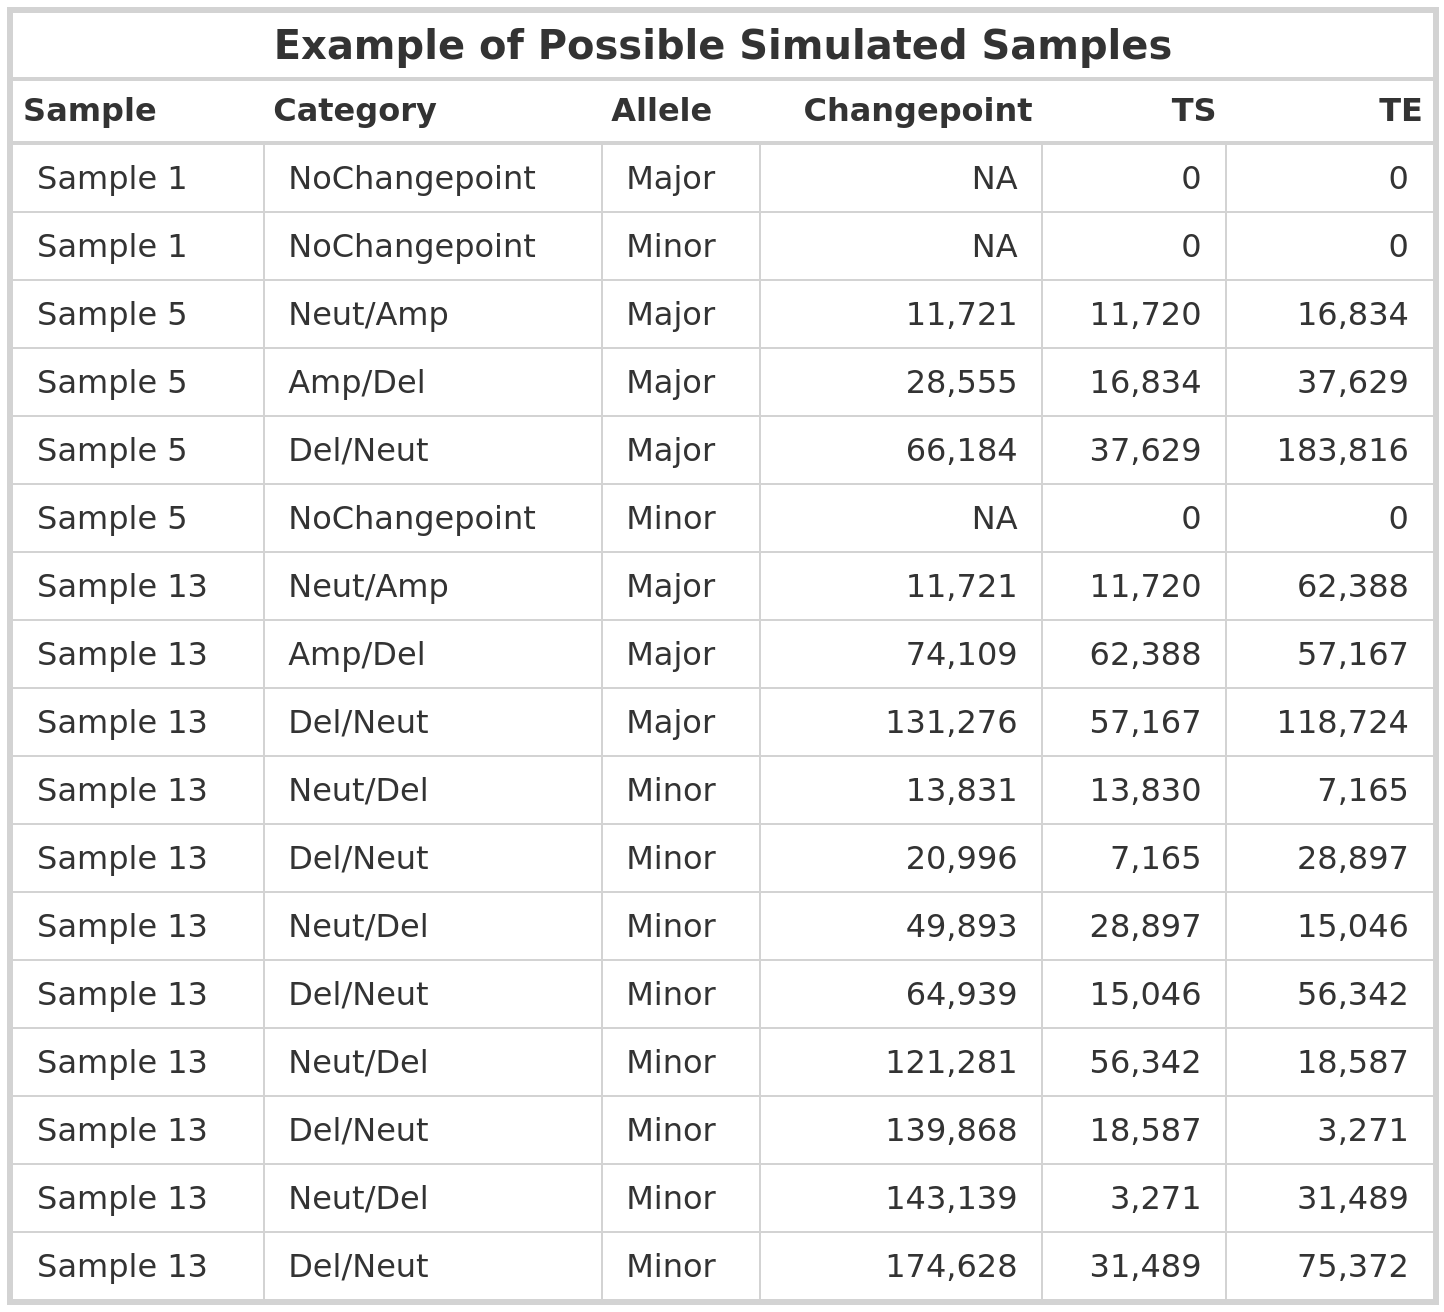
\includegraphics[width = 1\textwidth]{../tables/Chapter_5/Indv_Simulated_Example_Neut.png}
    \end{subtable} 
    \label{tab:Model_Example}
\end{table}

\vspace{1cm}

\begin{table}[!htb]
\caption[Summary statistics by category of the simulated dataset.]{Summary statistics by category of the simulated dataset. In (A) the lengths of the neutral segments are recorded as length 0 and in (B) the lengths of the neutral segments are retained as length greater than 0.} 
\label{tbl:summary_scen3}
\begin{subtable}{1\textwidth}
\centering
 \caption{Dataset where neutral segment length recorded as length 0.}\label{tab:sub_first}
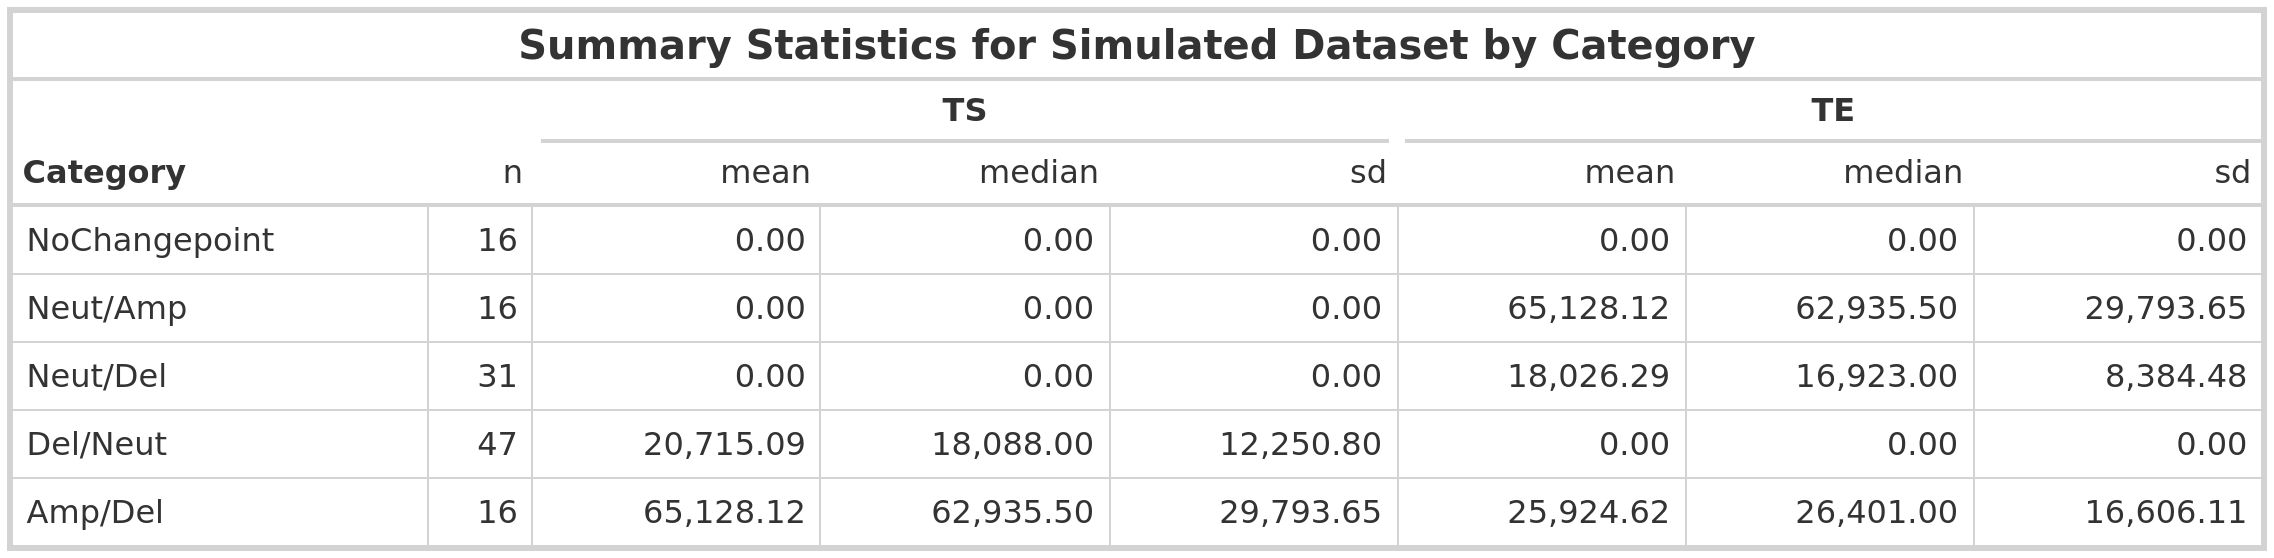
\includegraphics[width = 1\textwidth]{../tables/Chapter_5/Indv_Simulated_Example_Summary_Table_NoNeut.png}
\end{subtable}

\bigskip
\begin{subtable}{1\textwidth}
\caption{Dataset where neutral segment lengths are retained as length greater than 0.}\label{tab:sub_second}
\centering
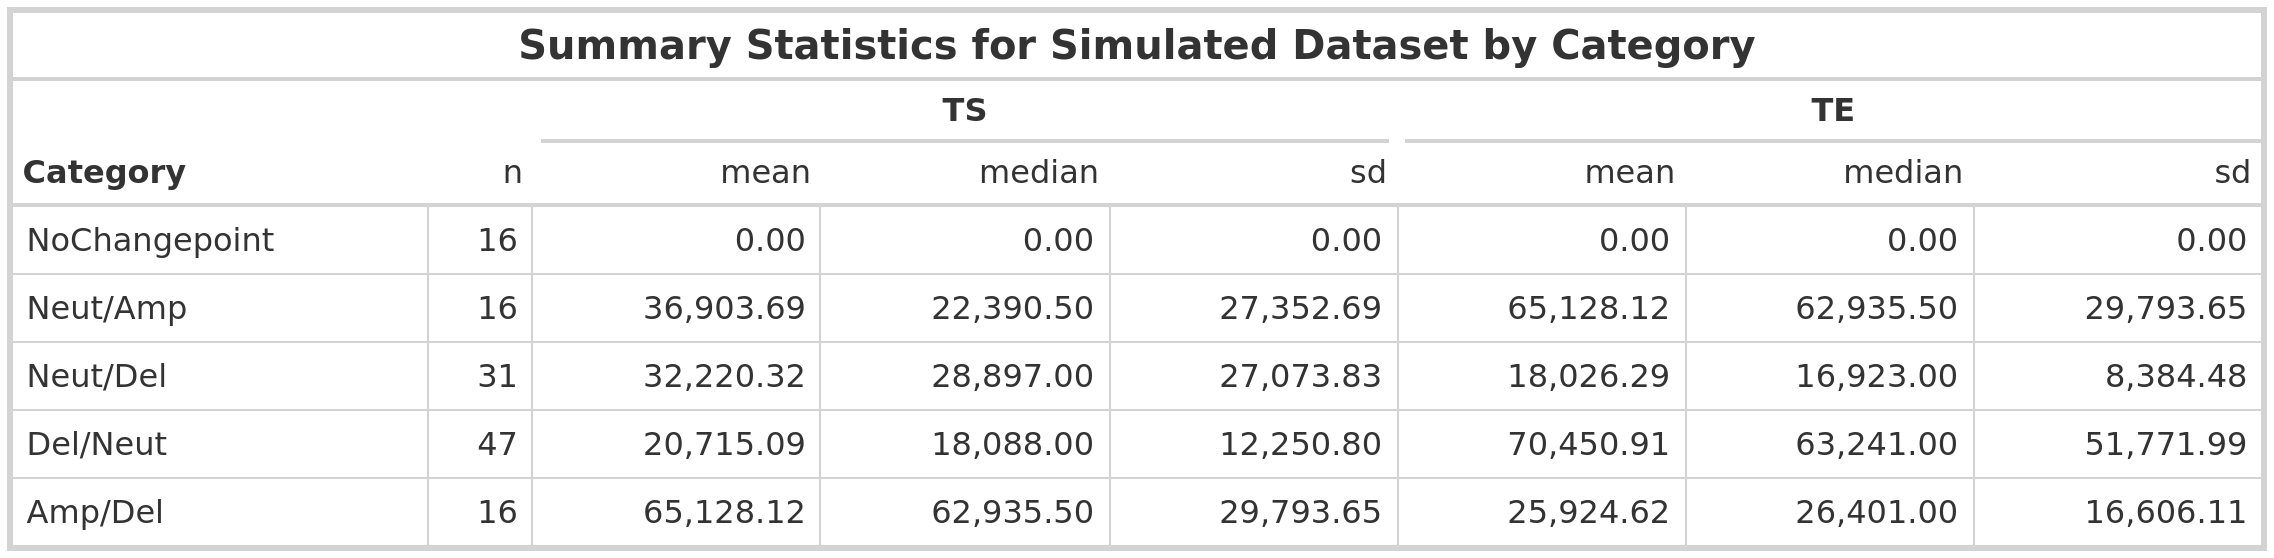
\includegraphics[width = 1\textwidth]{../tables/Chapter_5/Indv_Simulated_Example_Summary_Table_Neut.png}
\end{subtable}

\label{tab:three_tables}
\end{table}
\vfill 
\clearpage

Fitting the univariate AIIM to the data, using the \texttt{lm()} function, produces model parameter estimates provided in Table \ref{tbl:lm_uni_1_model}A. Table \ref{tbl:lm_uni_1_pred}A and Figure \ref{fig:lm_uni_1_int}A summarise interval estimates for these parameters. Table \ref{tbl:lm_uni_1_pred}A shows agreement between the parameter estimates and the mean lengths of the $TS$ and $TE$ recorded in Table \ref{tab:three_tables} across all categories, indicating that our fitted models are estimating the parameters as intended. The parameter estimates and confidence intervals demonstrate that the mean lengths of $TS$ for the Del/Neut and Amp/Del categories and the mean lengths of the $TE$ for the Neut/Del, Neut/Amp and Amp/Del categories are all significantly greater than 0. Tables \ref{tbl:lm_uni_1_model}B, \ref{tbl:lm_uni_1_pred}B and Figure \ref{fig:lm_uni_1_int}B provide the model parameter and interval estimates produced using the dataset where the lengths of the neutral segments are retained as length greater than 0. The parameter estimates and confidence intervals demonstrate that the mean lengths of $TS$ and $TE$ for all categories, excluding the NoChangepoint category, are estimated to be significantly different from 0 (Table \ref{tbl:lm_uni_1_pred}B and Figure \ref{fig:lm_uni_1_int}B). Retaining the lengths of the neutral segments, which are often extremely variable in length, results in an increased variance within the dataset, leading to wider, less precise, interval estimates for all categories. Although these intervals are wider, it is important to note that apart from the detection of the neutral segments, the conclusions do not change, i.e. the categories detected as having mean length(s) significantly greater than 0 are the same. 

\vfill 
\begin{table}[!htb]
    \caption[Univariate Allele-Independent Intercept Model parameter estimates fitted using \texttt{lm()}.]{Univariate Allele-Independent Intercept Model parameter estimates fitted using \texttt{lm()}. In (A) neutral lengths are recorded as length 0 and in (B) neutral lengths are retained as greater than 0.}
    \label{tbl:lm_uni_1_model}
     \begin{subtable}[t]{.49\textwidth}
      \centering
      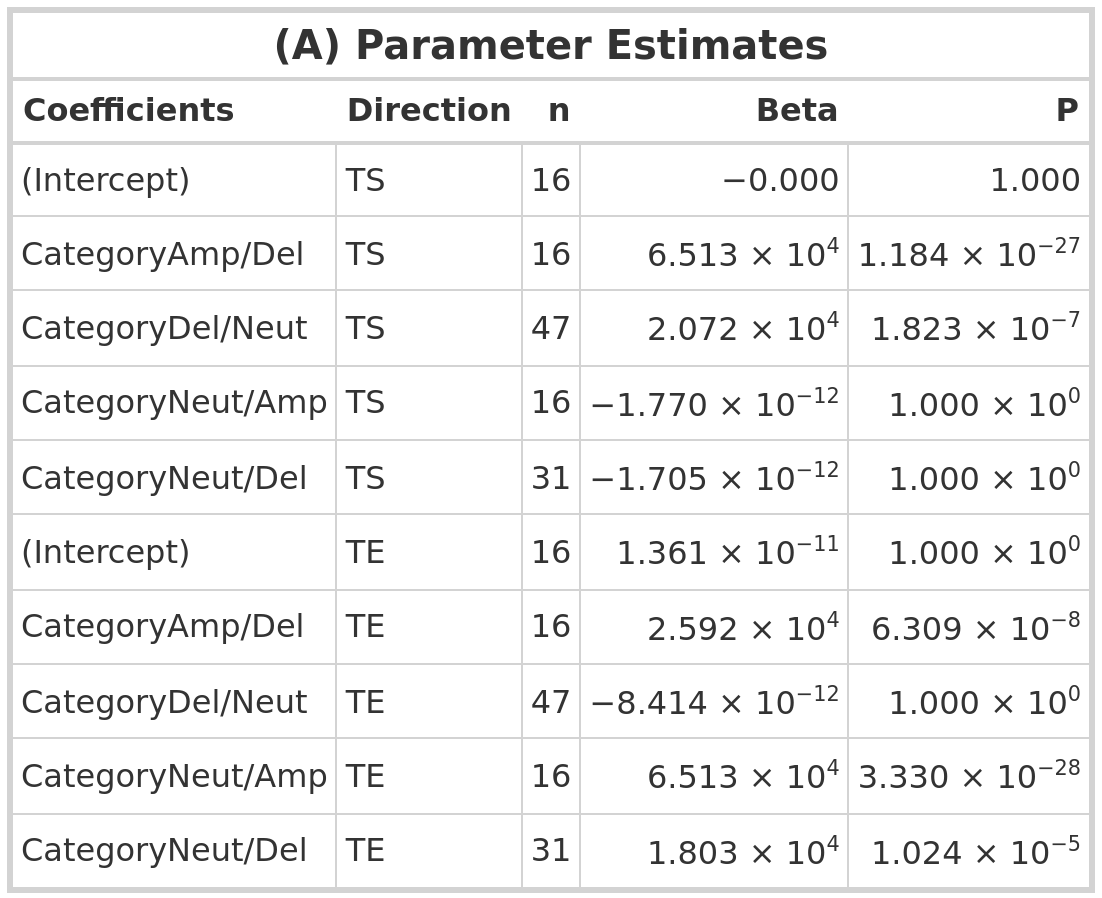
\includegraphics[width = 1\textwidth]{../tables/Chapter_5/Univariate_lm_7_AI_Model.png}
    \end{subtable}%
    \hspace{0.5cm}
     \begin{subtable}[t]{.49\textwidth}
      \centering
         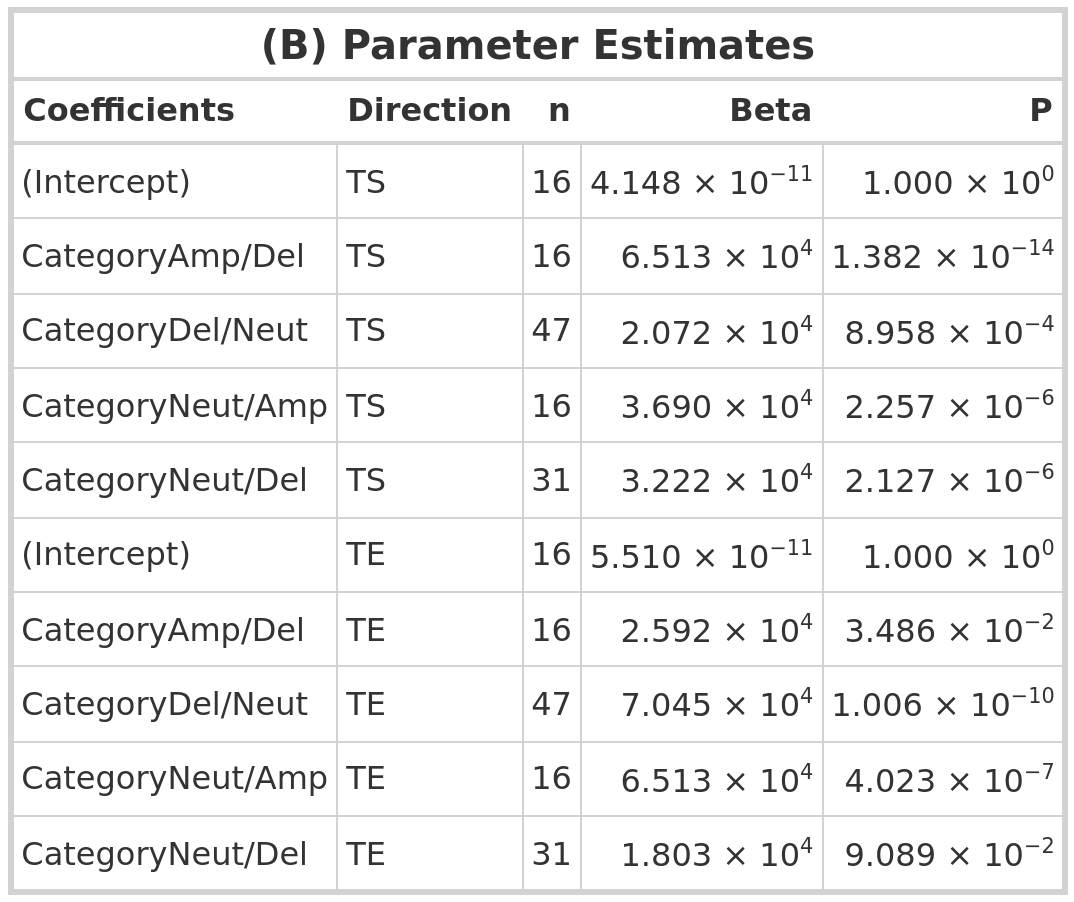
\includegraphics[width = 1\textwidth]{../tables/Chapter_5/Univariate_lm_7_Neut_AI_Model.png}
    \end{subtable} 
\end{table}
\vfill 
\clearpage

\begin{table}[!htb]
    \caption[Univariate Allele-Independent Intercept Model parameter estimates and intervals fitted using \texttt{lm()}.]{Univariate Allele-Independent Intercept Model parameter estimates and intervals fitted using \texttt{lm()}. In (A) neutral lengths are recorded as length 0 and in (B) neutral lengths are retained as greater than 0. Fit, LB and UB correspond to the parameter estimates and associated 95\% confidence intervals. }
    \label{tbl:lm_uni_1_pred}
     \begin{subtable}[t]{.49\textwidth}
      \centering
      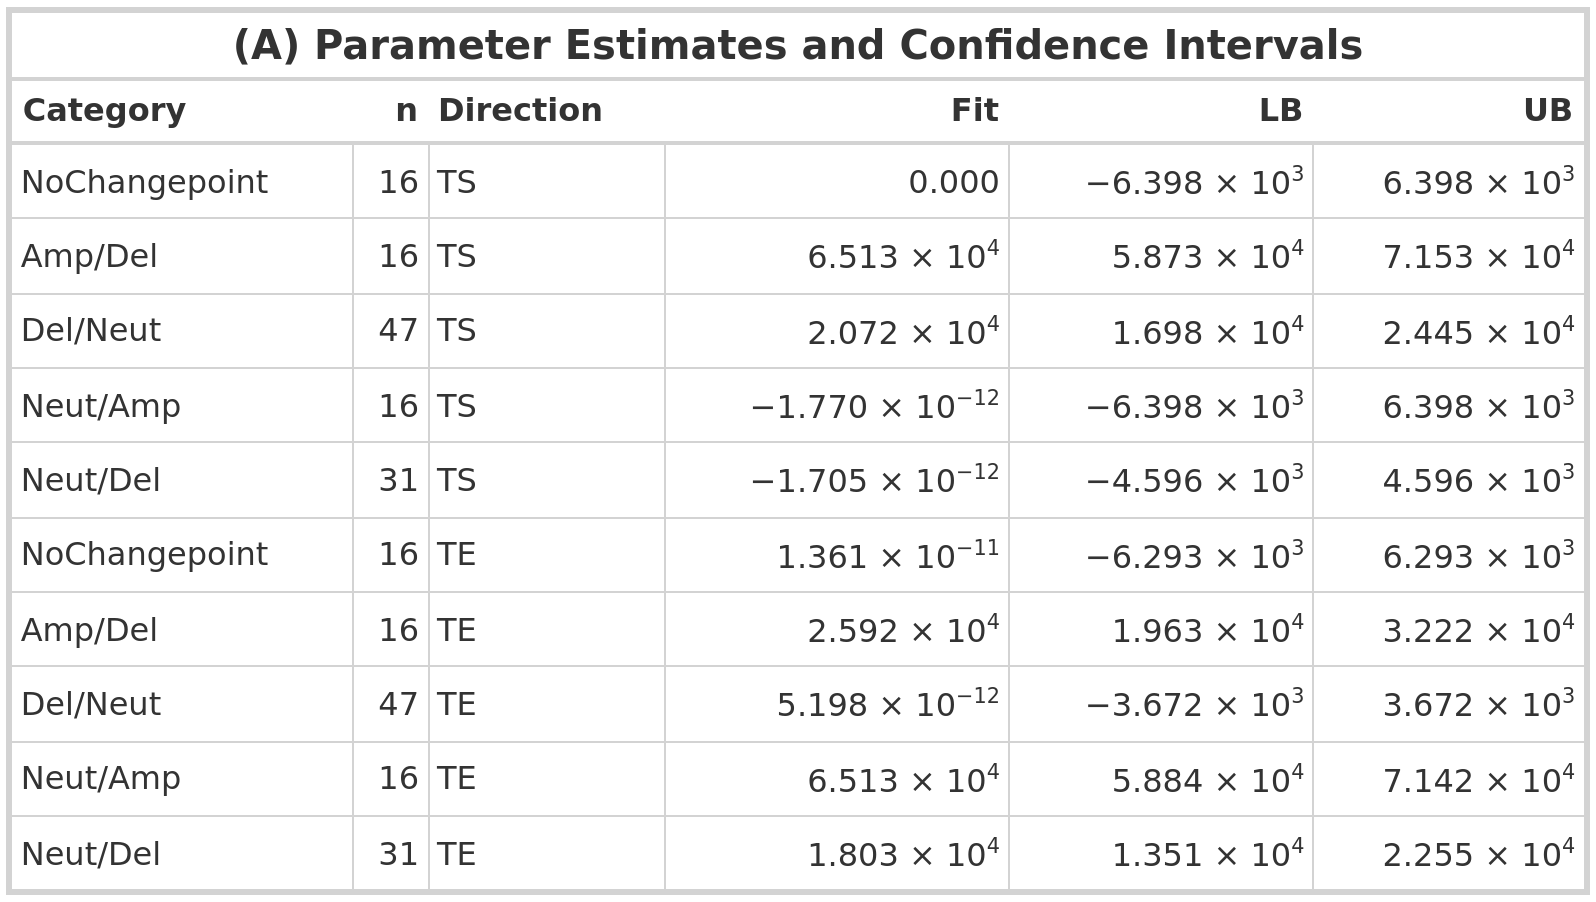
\includegraphics[width = 1\textwidth]{../tables/Chapter_5/Univariate_lm_7_AI_Pred.png}
    \end{subtable}%
    \hspace{0.5cm}
     \begin{subtable}[t]{.49\textwidth}
      \centering
         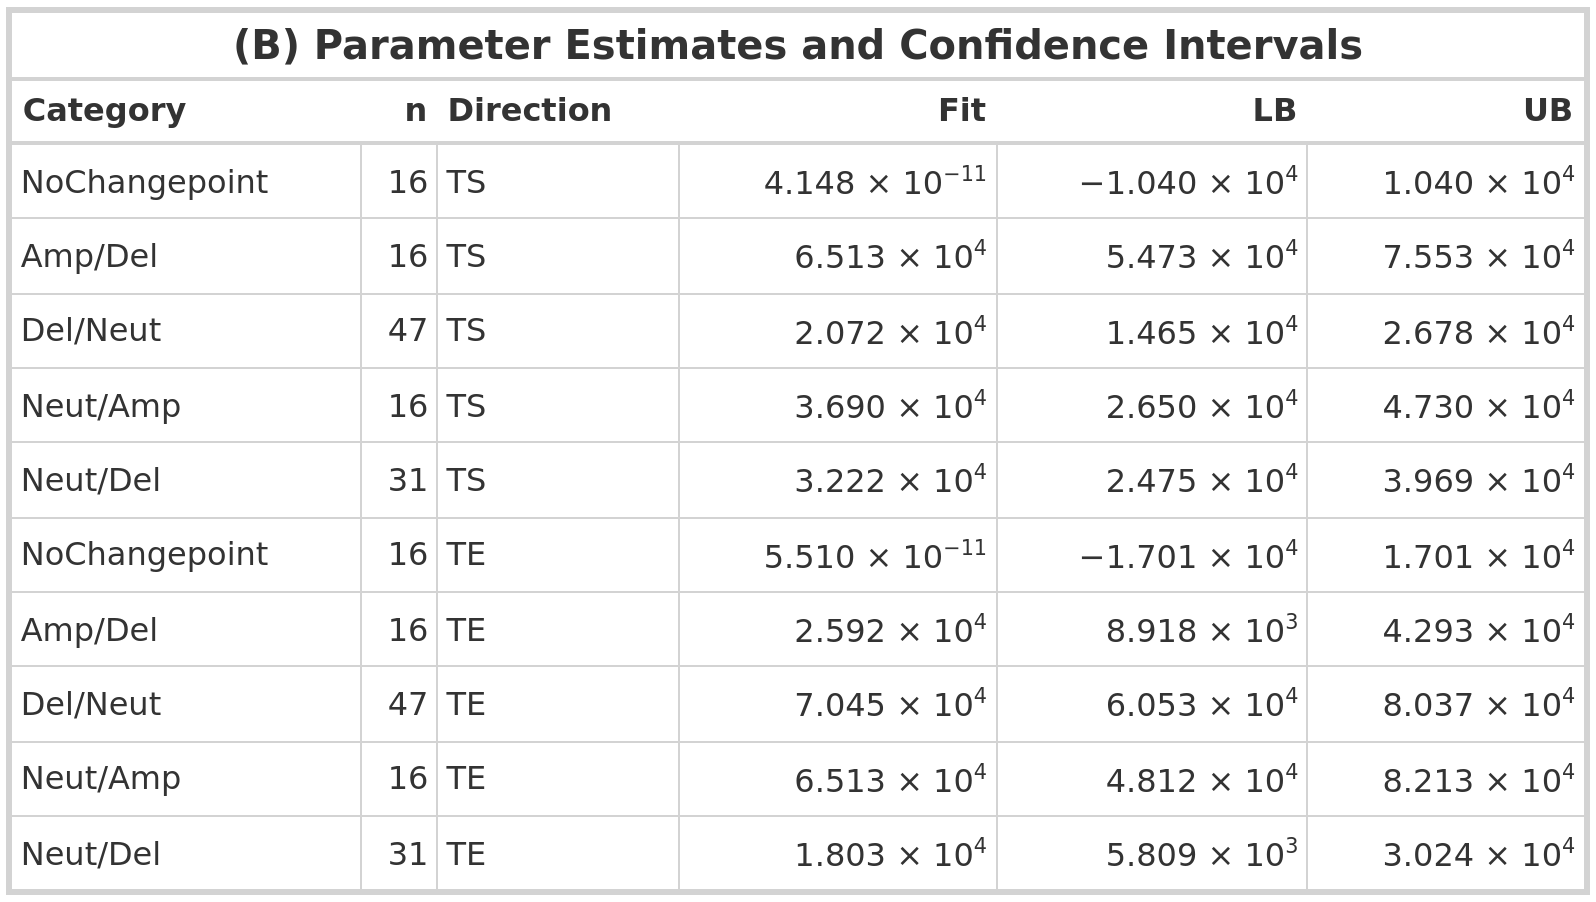
\includegraphics[width = 1\textwidth]{../tables/Chapter_5/Univariate_lm_7_Neut_AI_Pred.png}
    \end{subtable} 
\end{table}

\begin{figure}[H]
\vspace{0.5cm}
     \begin{subfigure}[t]{.49\textwidth}
      \centering
      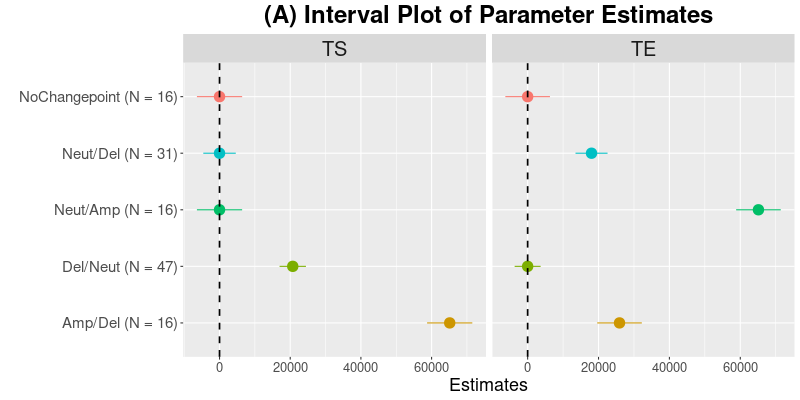
\includegraphics[width = 1\textwidth]{../figures/Chapter_5/Univariate_lm_7_AI_Interval.png}
    \end{subfigure}%
     \begin{subfigure}[t]{.49\textwidth}
      \centering
       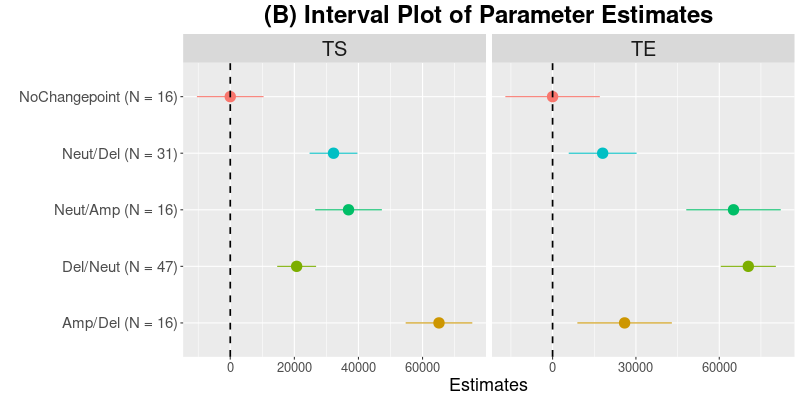
\includegraphics[width = 1\textwidth]{../figures/Chapter_5/Univariate_lm_7_Neut_AI_Interval.png}
    \end{subfigure} 
     \caption[Interval plot of univariate Allele-Independent Intercept Model parameter estimates fitted using \texttt{lm()}.]{Interval plot of univariate Allele-Independent Intercept Model parameter estimates fitted using \texttt{lm}. In (A) neutral lengths are recorded as length 0 and in (B) neutral lengths are retained as greater than 0.}
     \label{fig:lm_uni_1_int}
\end{figure}

Focusing on the application in which a variant of the dataset excludes all NoChangepoint observations, and fitting the univariate AINIM gives parameter estimates, as provided in Table \ref{tbl:lm_uni_2_model}, and confidence interval estimates (Table \ref{tbl:lm_uni_2_pred} and Figure  \ref{fig:lm_uni_2_int}).

The results of the AINIM are similar to the AIIM, with the parameter estimates corresponding to the mean lengths of the $TS$ and $TE$ recorded in Table \ref{tab:three_tables} across all categories, and the interval plots, highlighting the categories where the lower bound of the confidence interval is greater than 0. Utilising the dataset where the neutral lengths are recorded as 0, the mean lengths of $TS$ for the Del/Neut and Amp/Del categories and the mean lengths of the $TE$ for the Neut/Del, Neut/Amp and Amp/Del categories are all significantly greater than 0. When utilising the dataset where the neutral lengths are retained as greater than 0, the mean lengths of $TS$ and $TE$ for all categories are significantly greater than 0. The main consequences of removing the NoChangepoint observations are the reduction in sample size and the increased width of the confidence intervals in the AINIM, compared to the AIIM, due to the removal of a large number of constant 0 values leading to an increase in variance in the dataset. 

The results obtained for the univariate AIIM and AINIM, fitted using the \texttt{MCMCglmm()} function, show similar behaviour, with the same categories being highlighted as significant (Appendix E).

\vfill 
\begin{table}[H]
\vspace{0.8cm}
    \caption[Univariate Allele-Independent Non-Intercept Model parameter estimates fitted using \texttt{lm()}.]{Univariate Allele-Independent Non-Intercept Model parameter estimates fitted using \texttt{lm()}. In (A) neutral lengths are recorded as length 0 and in (B) neutral lengths are retained as greater than 0.}
    \label{tbl:lm_uni_2_model}
     \begin{subtable}[t]{.49\textwidth}
      \centering
      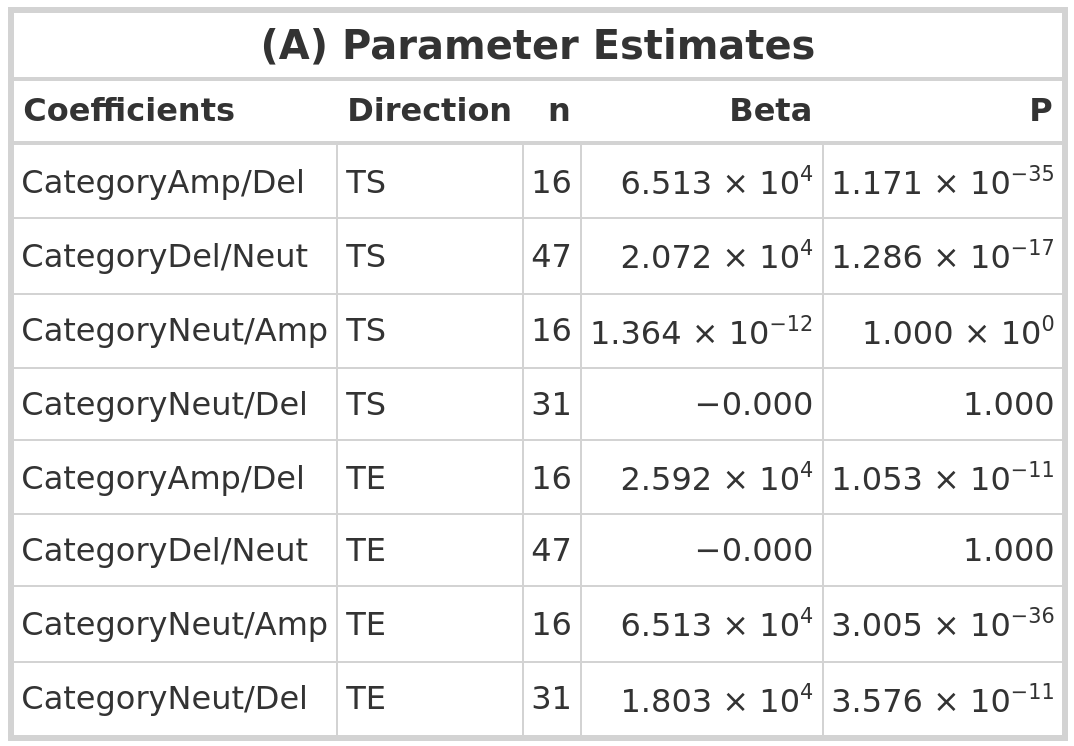
\includegraphics[width = 1\textwidth]{../tables/Chapter_5/Univariate_lm_6_AI_Model.png}
    \end{subtable}%
    \hspace{0.5cm}
     \begin{subtable}[t]{.49\textwidth}
      \centering
         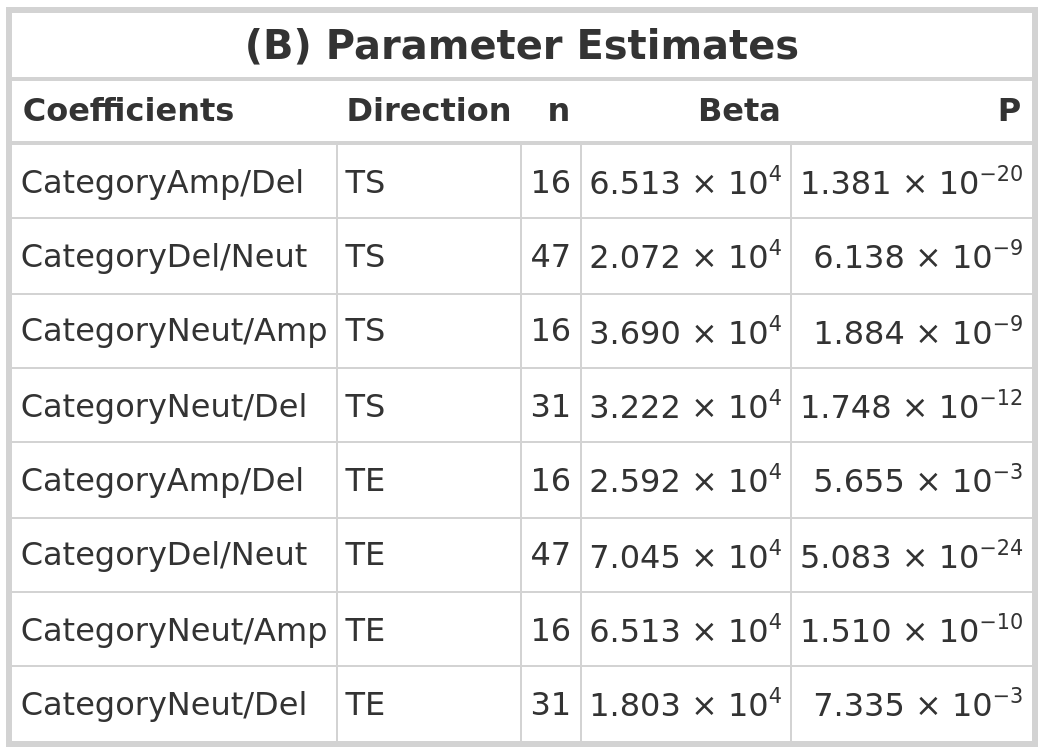
\includegraphics[width = 1\textwidth]{../tables/Chapter_5/Univariate_lm_6_Neut_AI_Model.png}
    \end{subtable} 
\end{table}

\begin{table}[H]
\vspace{0.5cm}
    \caption[Univariate Allele-Independent Non-Intercept Model parameter estimates and intervals fitted using \texttt{lm()}.]{Univariate Allele-Independent Non-Intercept Model parameter estimates and intervals fitted using \texttt{lm()}. In (A) neutral lengths are recorded as length 0 and in (B) neutral lengths are retained as greater than 0. Fit, LB and UB correspond to the parameter estimates and associated 95\% confidence intervals. }
    \label{tbl:lm_uni_2_pred}
     \begin{subtable}[t]{.49\textwidth}
      \centering
      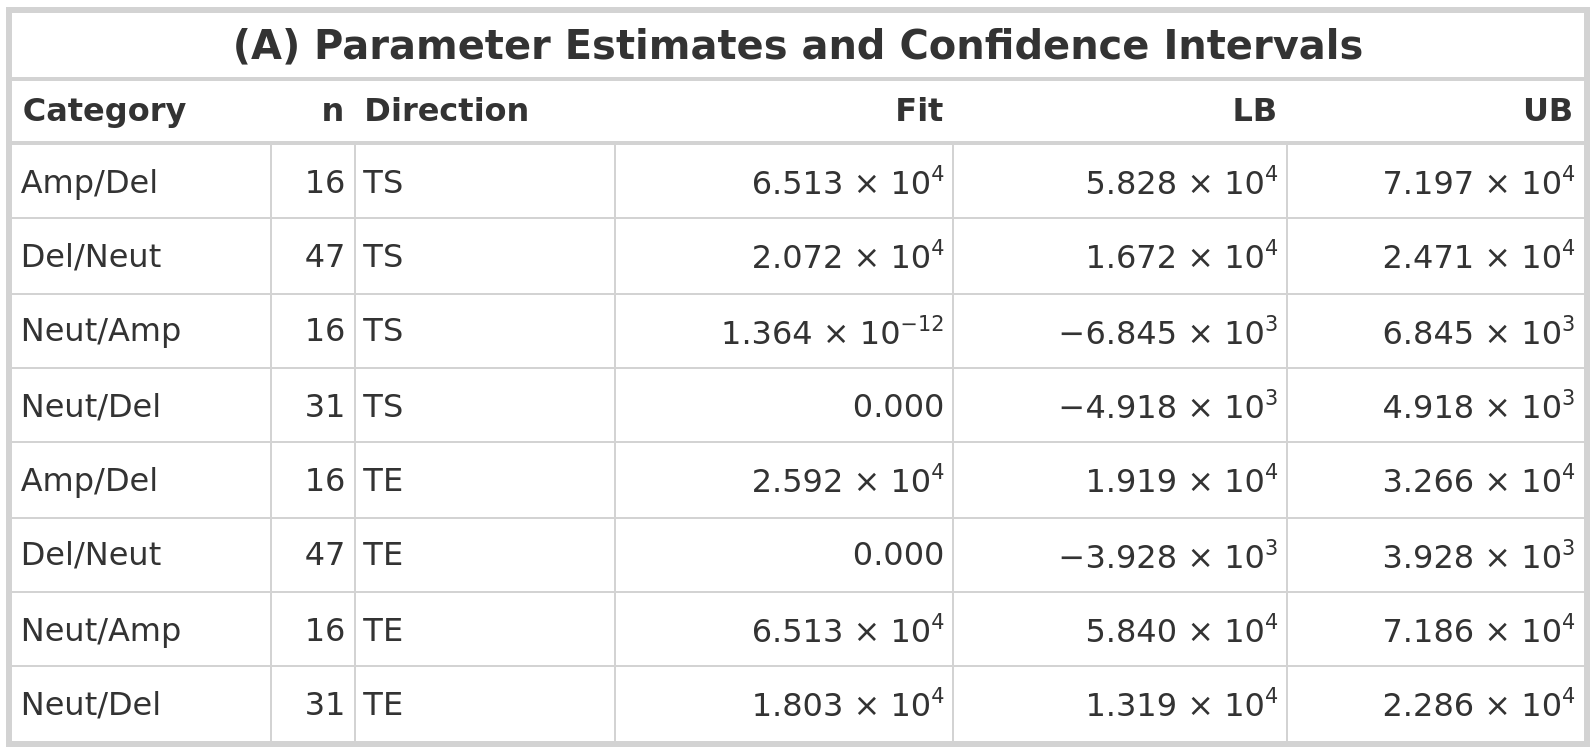
\includegraphics[width = 1\textwidth]{../tables/Chapter_5/Univariate_lm_6_AI_Pred.png}
    \end{subtable}%
    \hspace{0.5cm}
     \begin{subtable}[t]{.49\textwidth}
      \centering
         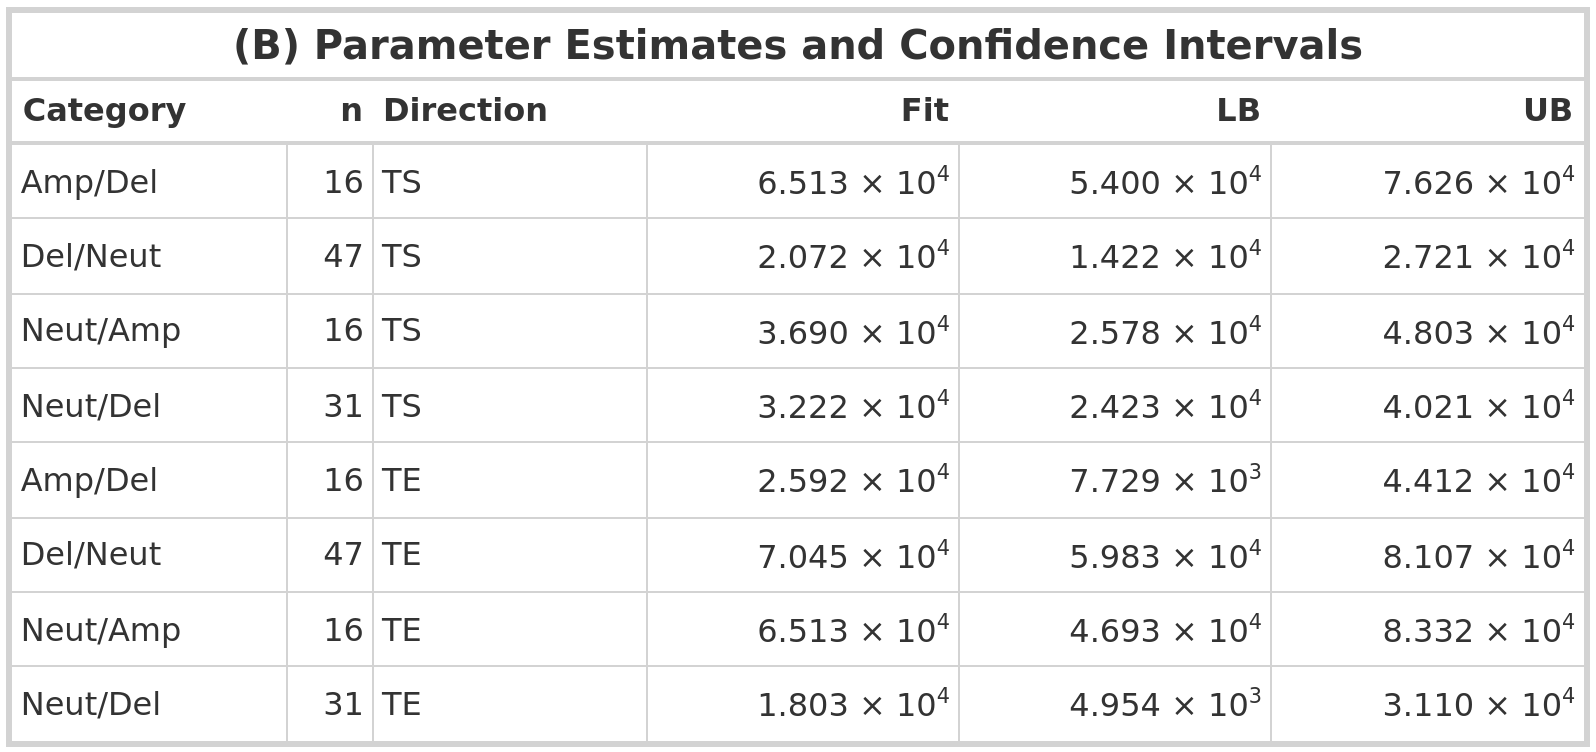
\includegraphics[width = 1\textwidth]{../tables/Chapter_5/Univariate_lm_6_Neut_AI_Pred.png}
    \end{subtable} 
\end{table}

\begin{figure}[H]
\vspace{0.7cm}
     \begin{subfigure}[t]{.49\textwidth}
      \centering
      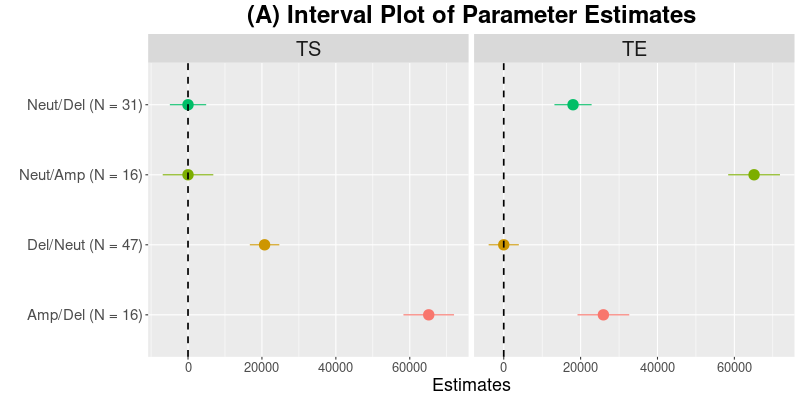
\includegraphics[width = 1\textwidth]{../figures/Chapter_5/Univariate_lm_6_AI_Interval.png}
    \end{subfigure}%
     \begin{subfigure}[t]{.49\textwidth}
      \centering
       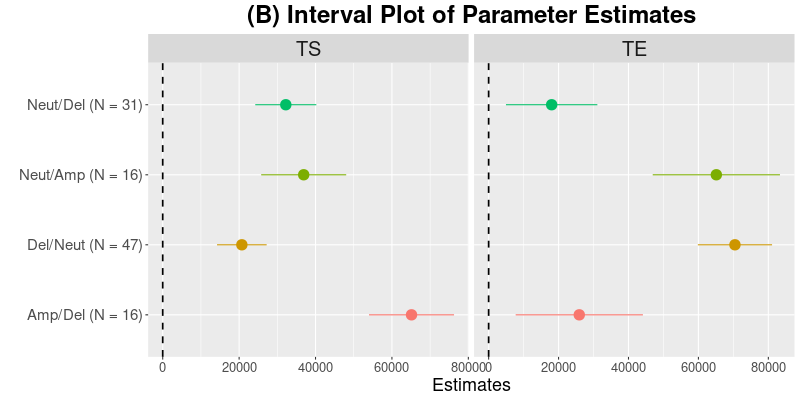
\includegraphics[width = 1\textwidth]{../figures/Chapter_5/Univariate_lm_6_Neut_AI_Interval.png}
    \end{subfigure} 
     \caption[Interval plot of univariate Allele-Independent Non-Intercept Model parameter estimates fitted using \texttt{lm()}.]{Interval plot of univariate Allele-Independent Non-Intercept Model parameter estimates fitted using \texttt{lm()}. In (A) neutral lengths are recorded as length 0 and in (B) neutral lengths are retained as greater than 0.}
     \label{fig:lm_uni_2_int}
\end{figure}
\vfill 

\clearpage

Fitting the multivariate AIIM and AINIM to the data identifies a limitation of the \texttt{predict()} function previously used to produce confidence intervals (Tables \ref{tbl:lm_multi_1_model}-\ref{tbl:lm_multi_2_pred} and Figures \ref{fig:lm_multi_1_int} and \ref{fig:lm_multi_2_int}). Obtaining confidence intervals for multivariate models fitted with the \texttt{lm()} function is not supported. As a result, only point estimates are shown in Tables \ref{tbl:lm_multi_1_model}-\ref{tbl:lm_multi_2_pred} and Figures \ref{fig:lm_multi_1_int} and \ref{fig:lm_multi_2_int}, with these point estimates mirroring those obtained from the univariate models.  

The \texttt{MCMCglmm()} function overcomes this limitation, and produces similar results, by enabling the production of confidence intervals for both the multivariate models using the \texttt{predict.MCMCglmm()} function (Appendix E). 

Overall, when comparing model fits where the neutral segment lengths are retained as greater than 0 and where the neutral segment lengths recorded as 0, there is increased detection of the changepoints with a neutral length and an increase in the width of the confidence intervals. Although these intervals are wider, it is important to note that apart from the detection of the neutral segments, the conclusions do not change, i.e. the categories detected as having mean length(s) significantly greater than 0 are the same in both instances. As the primary interest here is in CNA changepoints, focus is given to the dataset where the neutral segment lengths are recorded as 0.  

Notably, the \texttt{lm()} and \texttt{MCMCglmm()} functions perform similarly across the univariate AI models, but limitations in the \texttt{predict()} functions result in only the \texttt{predict.MCMCglmm()} function being capable of producing confidence intervals for multivariate models.

\vspace{1cm}
\begin{table}[H]
    \caption[Multivariate Allele-Independent Intercept Model parameter estimates fitted using \texttt{lm()}.]{Multivariate Allele-Independent Intercept Model parameter estimates fitted using \texttt{lm()}. In (A) neutral lengths are recorded as length 0 and in (B) neutral lengths are retained as greater than 0.}
    \label{tbl:lm_multi_1_model}
     \begin{subtable}[t]{.49\textwidth}
      \centering
      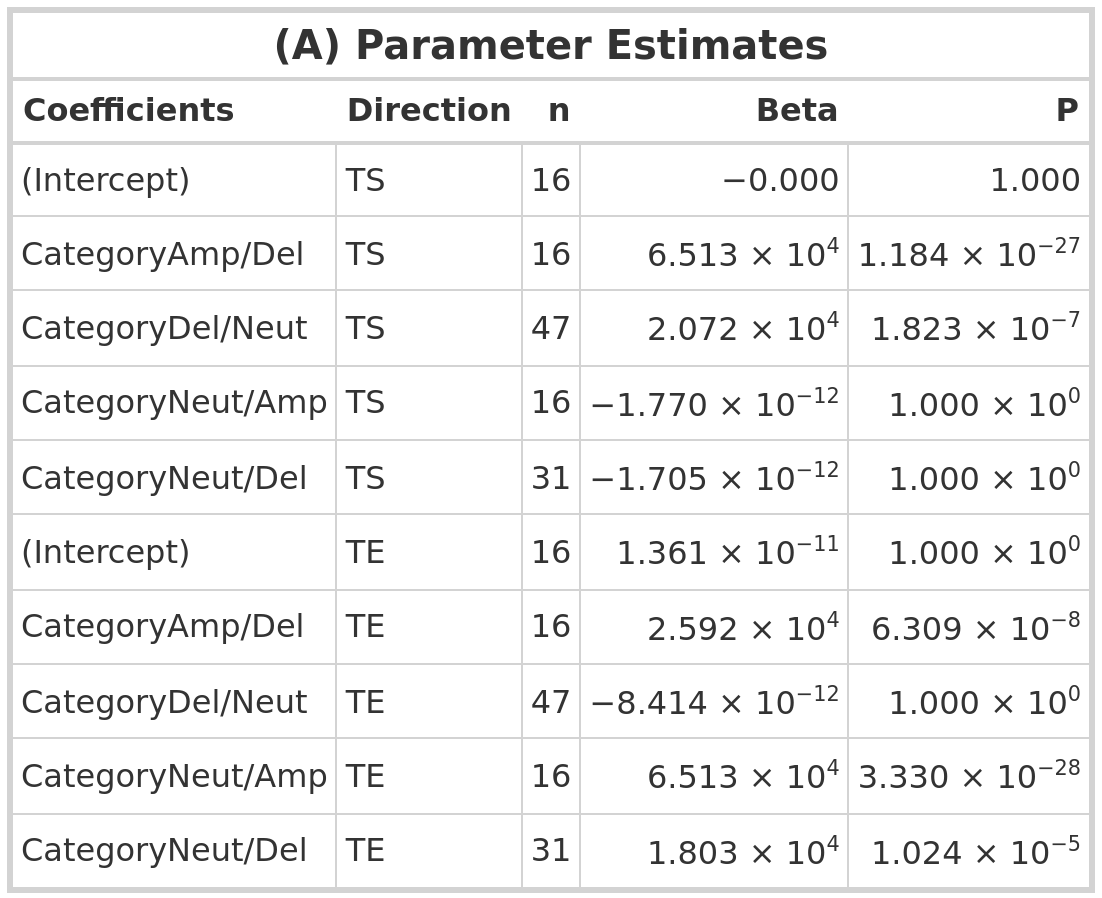
\includegraphics[width = 1\textwidth]{../tables/Chapter_5/Multivariate_lm_7_AI_Model.png}
    \end{subtable}%
    \hspace{0.5cm}
     \begin{subtable}[t]{.49\textwidth}
      \centering
         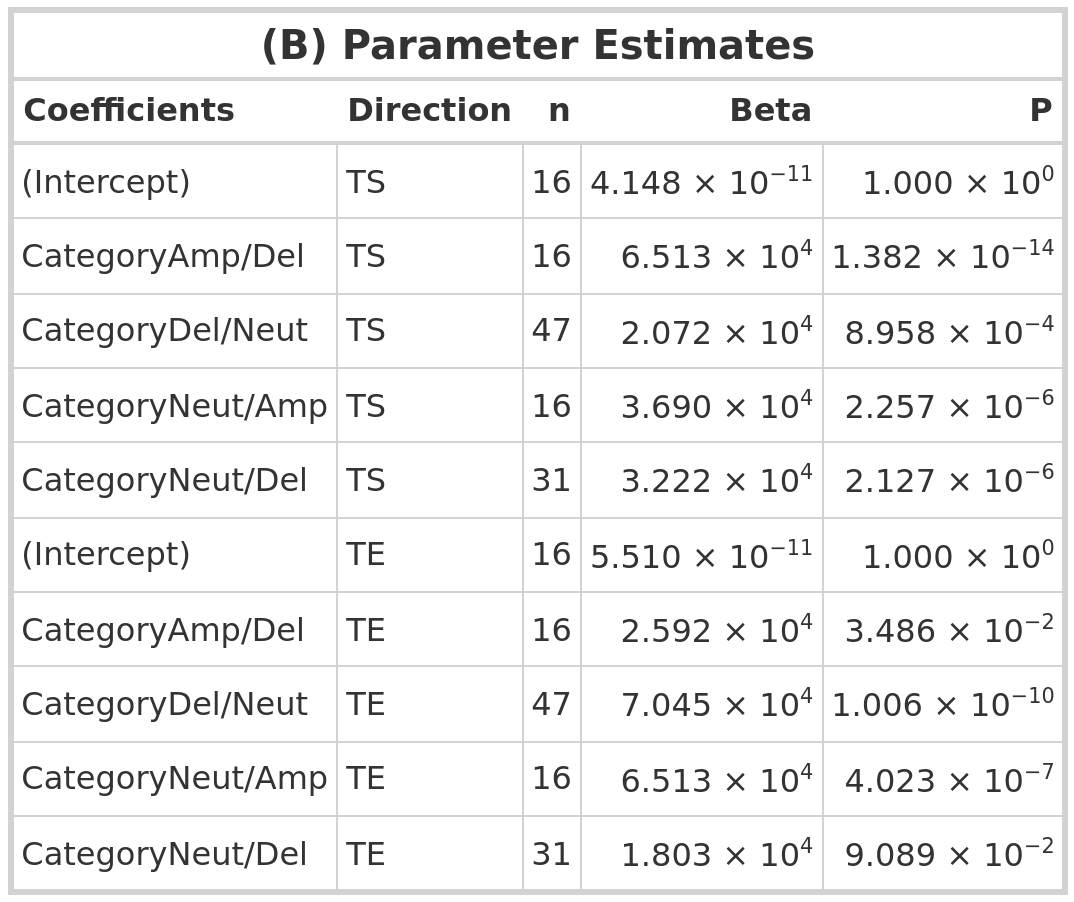
\includegraphics[width = 1\textwidth]{../tables/Chapter_5/Multivariate_lm_7_Neut_AI_Model.png}
    \end{subtable} 
\end{table}

\vfill 
\begin{table}[H]
    \caption[Multivariate Allele-Independent Intercept Model parameter estimates and intervals fitted using \texttt{lm()}.]{Multivariate Allele-Independent Intercept Model parameter estimates and intervals fitted using \texttt{lm()}. In (A) neutral lengths are recorded as length 0 and in (B) neutral lengths are retained as greater than 0. Fit, LB and UB correspond to the parameter estimates and associated 95\% confidence intervals. }
    \label{tbl:lm_multi_1_pred}
     \begin{subtable}[t]{.49\textwidth}
      \centering
      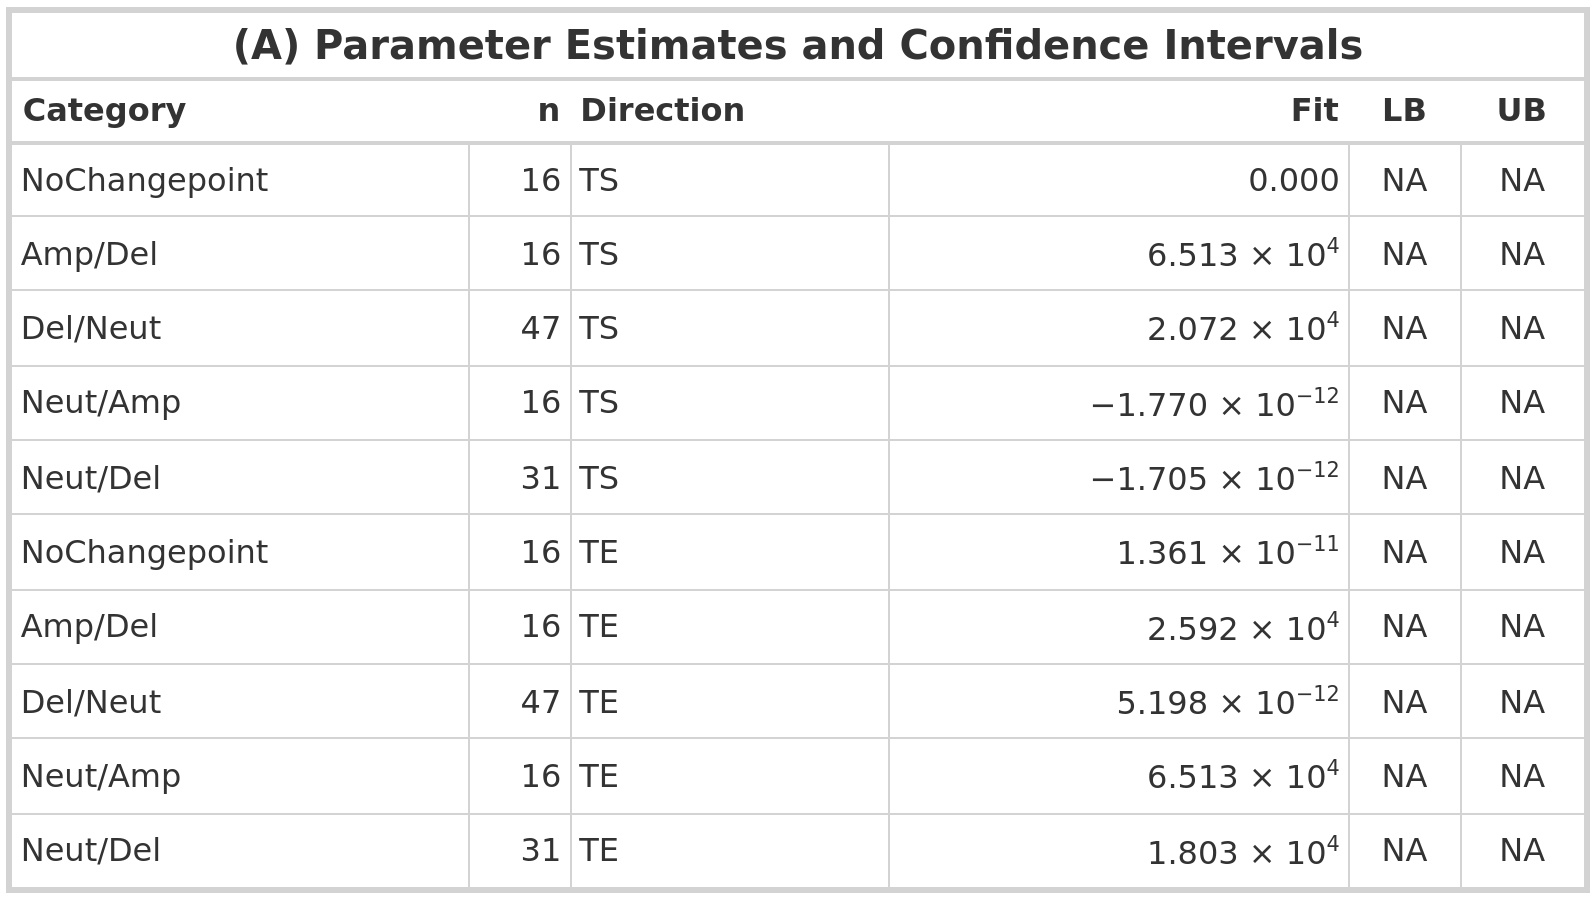
\includegraphics[width = 1\textwidth]{../tables/Chapter_5/Multivariate_lm_7_AI_Pred.png}
    \end{subtable}%
    \hspace{0.5cm}
     \begin{subtable}[t]{.49\textwidth}
      \centering
         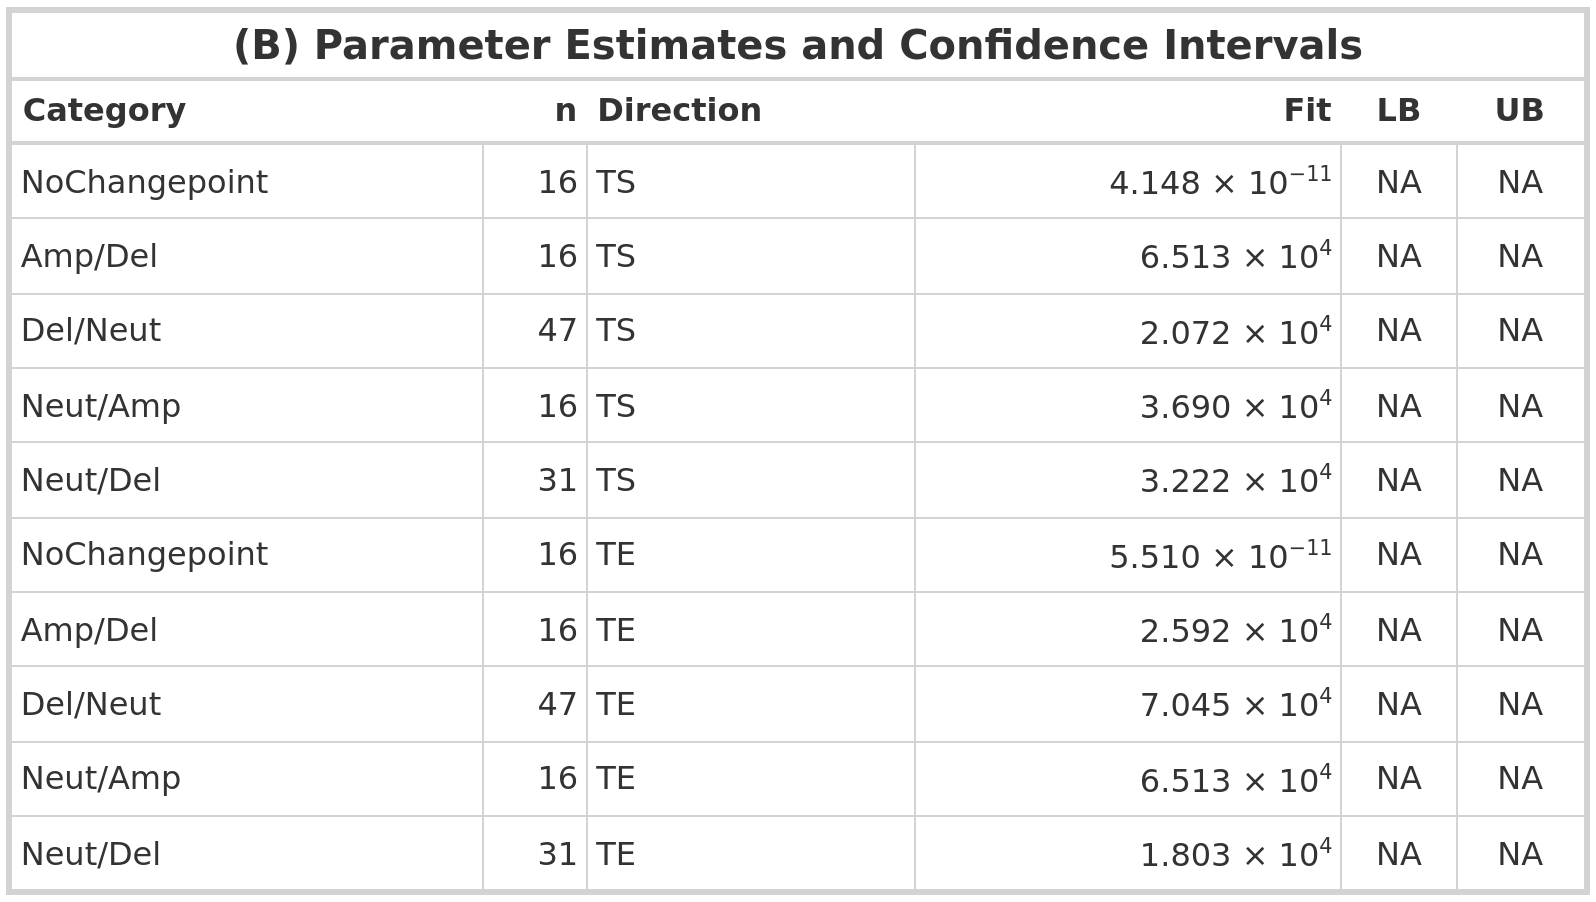
\includegraphics[width = 1\textwidth]{../tables/Chapter_5/Multivariate_lm_7_Neut_AI_Pred.png}
    \end{subtable} 
\end{table}

\begin{figure}[H]
\vspace{1cm}
     \begin{subfigure}[t]{.49\textwidth}
      \centering
      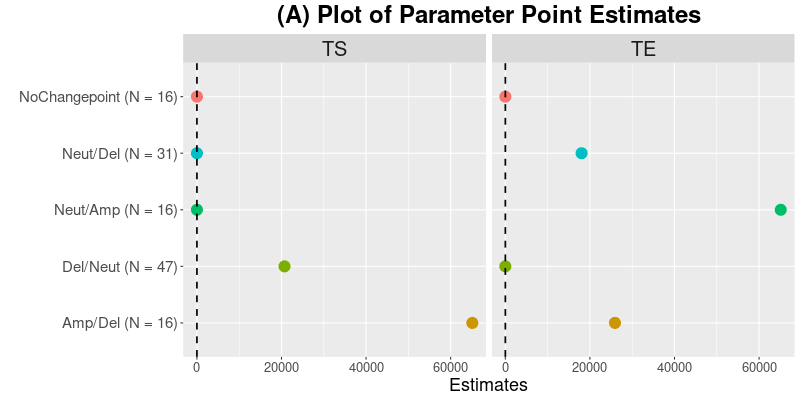
\includegraphics[width = 1\textwidth]{../figures/Chapter_5/Multivariate_lm_7_AI_Interval.png}
    \end{subfigure}%
     \begin{subfigure}[t]{.49\textwidth}
      \centering
       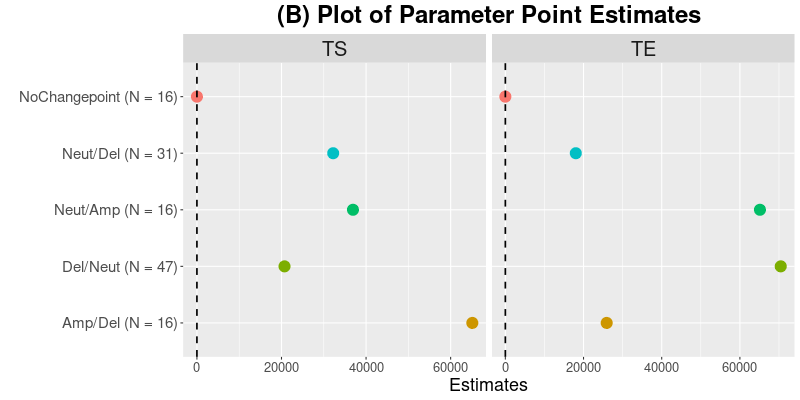
\includegraphics[width = 1\textwidth]{../figures/Chapter_5/Multivariate_lm_7_Neut_AI_Interval.png}
    \end{subfigure} 
     \caption[Plot of multivariate Allele-Independent Intercept Model parameter estimates fitted using \texttt{lm()}.]{Plot of multivariate Allele-Independent Intercept Model parameter estimates fitted using \texttt{lm()}. In (A) neutral lengths are recorded as length 0 and in (B) neutral lengths are retained as greater than 0.}
     \label{fig:lm_multi_1_int}
\end{figure}

\begin{table}[H]
\vspace{1cm}
    \caption[Multivariate Allele-Independent Non-Intercept Model parameter estimates fitted using \texttt{lm()}.]{Multivariate Allele-Independent Non-Intercept Model parameter estimates fitted using \texttt{lm()}. In (A) neutral lengths are recorded as length 0 and in (B) neutral lengths are retained as greater than 0.}
    \label{tbl:lm_multi_2_model}
     \begin{subtable}[t]{.49\textwidth}
      \centering
      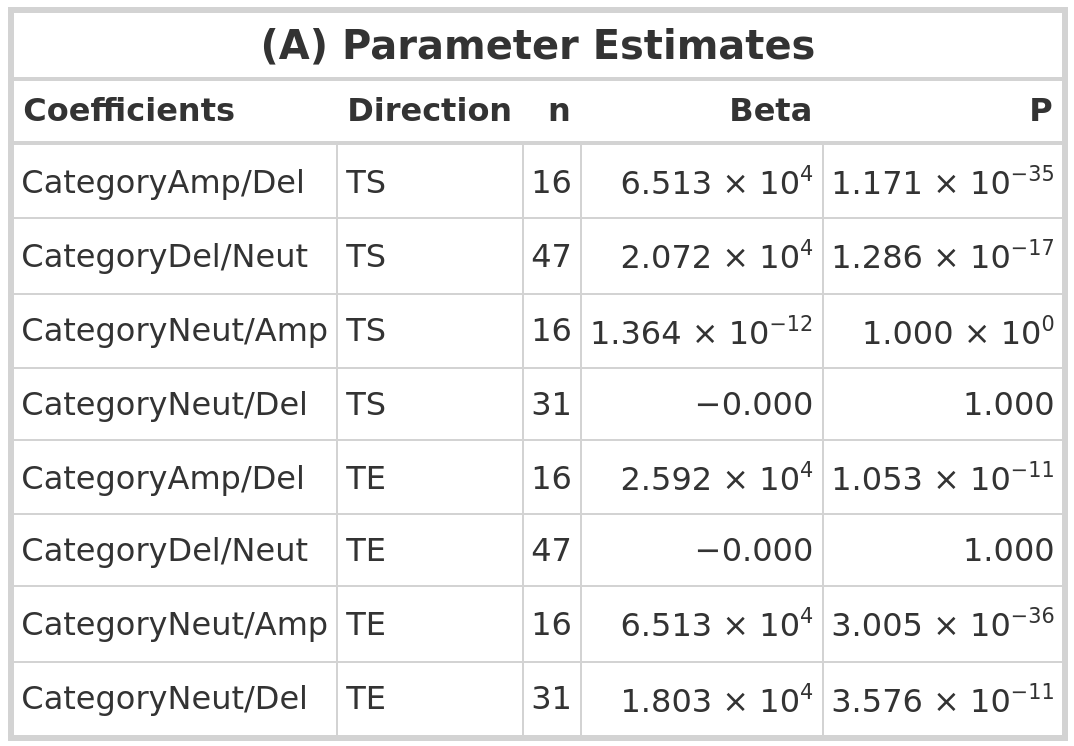
\includegraphics[width = 1\textwidth]{../tables/Chapter_5/Multivariate_lm_6_AI_Model.png}
    \end{subtable}%
    \hspace{0.5cm}
     \begin{subtable}[t]{.49\textwidth}
      \centering
         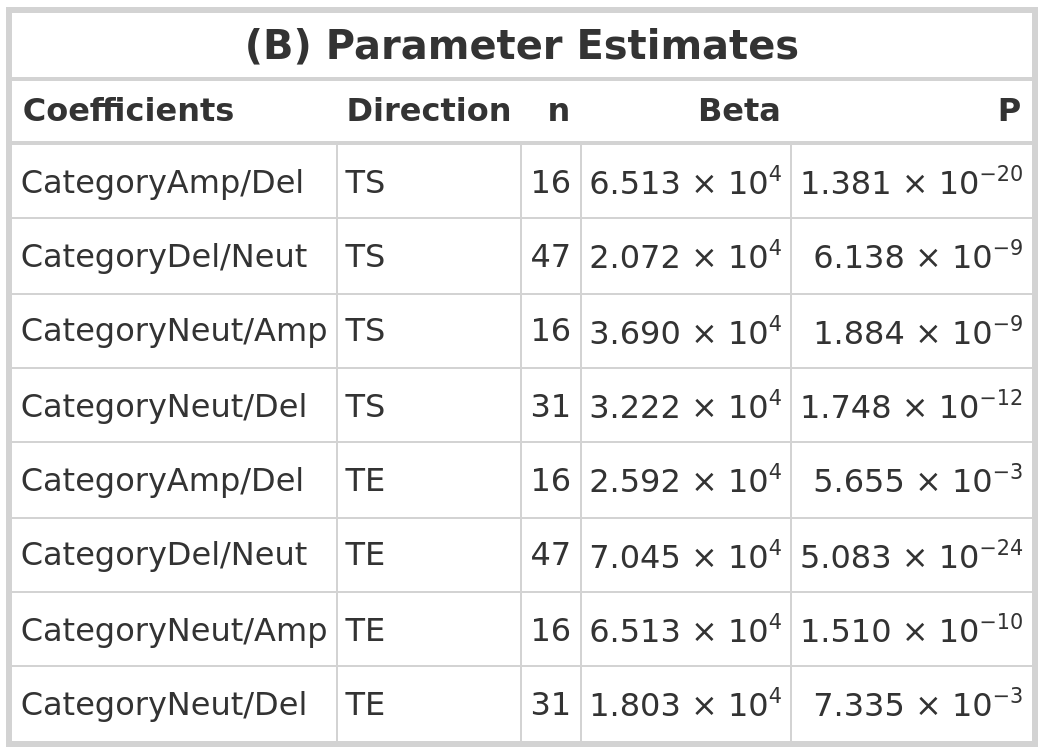
\includegraphics[width = 1\textwidth]{../tables/Chapter_5/Multivariate_lm_6_Neut_AI_Model.png}
    \end{subtable} 
\end{table}
\vfill 

\begin{table}[H]
    \caption[Multivariate Allele-Independent Non-Intercept Model parameter estimates and intervals fitted using \texttt{lm()}.]{Multivariate Allele-Independent Non-Intercept Model parameter estimates and intervals fitted using \texttt{lm()}. In (A) neutral lengths are recorded as length 0 and in (B) neutral lengths are retained as greater than 0. Fit, LB and UB correspond to the parameter estimates and associated 95\% confidence intervals. }
    \label{tbl:lm_multi_2_pred}
     \begin{subtable}[t]{.49\textwidth}
      \centering
      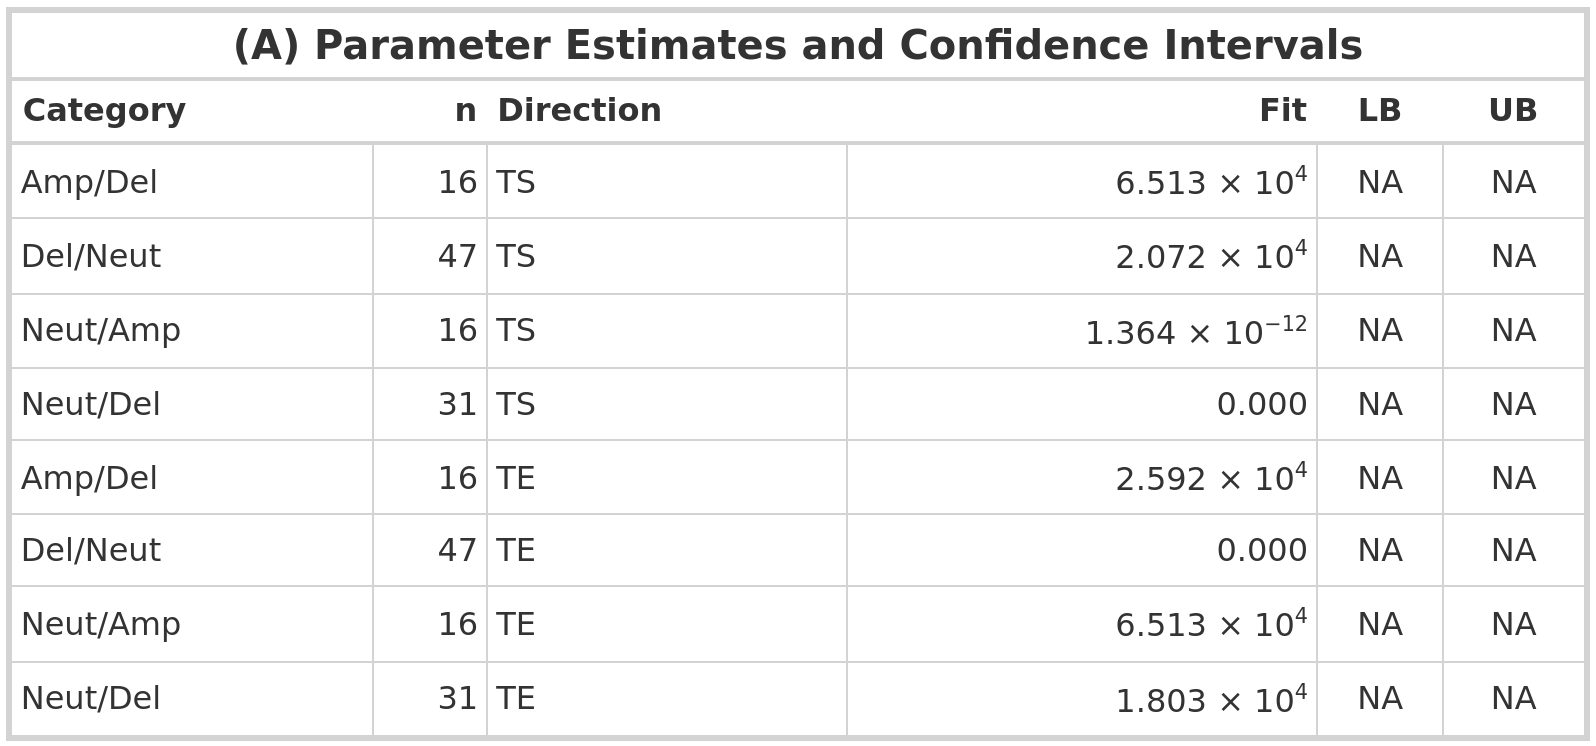
\includegraphics[width = 1\textwidth]{../tables/Chapter_5/Multivariate_lm_6_AI_Pred.png}
    \end{subtable}%
    \hspace{0.5cm}
     \begin{subtable}[t]{.49\textwidth}
      \centering
         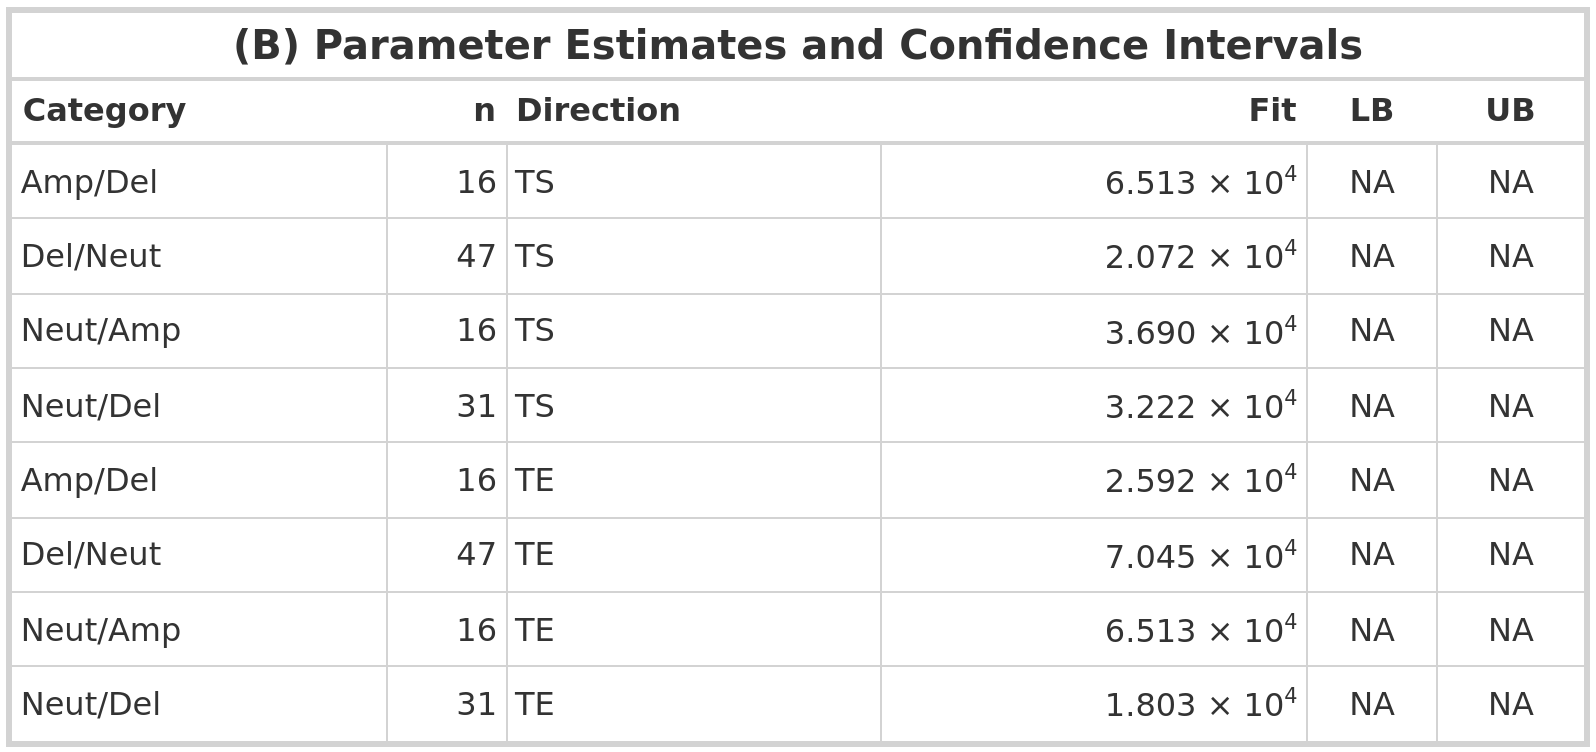
\includegraphics[width = 1\textwidth]{../tables/Chapter_5/Multivariate_lm_6_Neut_AI_Pred.png}
    \end{subtable} 
\end{table}

\begin{figure}[H]
\vspace{0.5cm}
     \begin{subfigure}[t]{.49\textwidth}
      \centering
      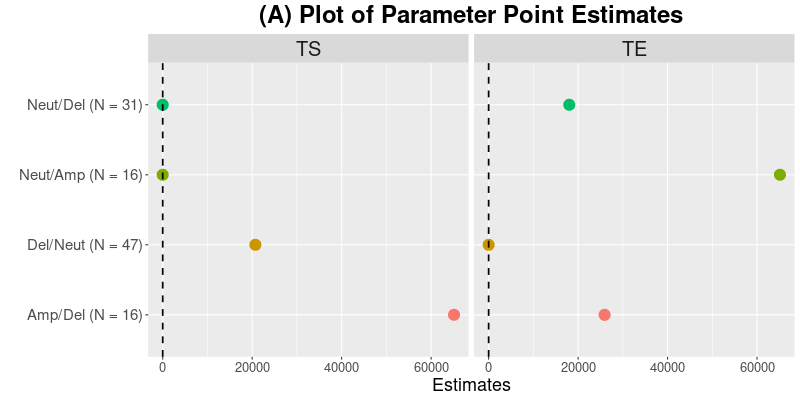
\includegraphics[width = 1\textwidth]{../figures/Chapter_5/Multivariate_lm_6_AI_Interval.png}
    \end{subfigure}%
     \begin{subfigure}[t]{.49\textwidth}
      \centering
       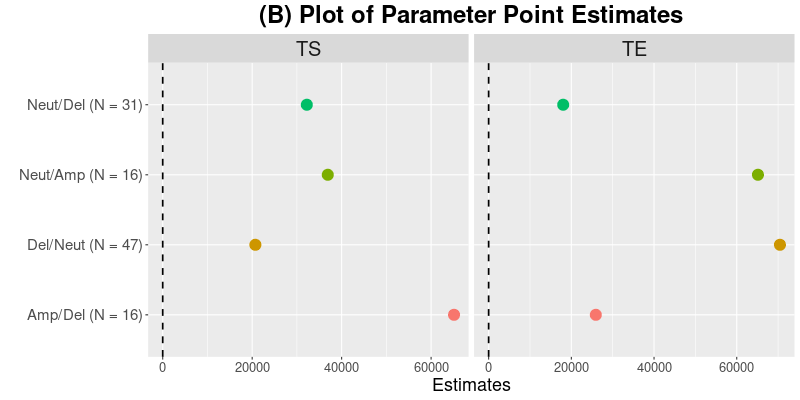
\includegraphics[width = 1\textwidth]{../figures/Chapter_5/Multivariate_lm_6_Neut_AI_Interval.png}
    \end{subfigure} 
     \caption[Plot of multivariate Allele-Independent Non-Intercept Model parameter estimates fitted using \texttt{lm()}.]{Plot of multivariate Allele-Independent Non-Intercept Model parameter estimates fitted using \texttt{lm()}. In (A) neutral lengths are recorded as length 0 and in (B) neutral lengths are retained as greater than 0.}
     \label{fig:lm_multi_2_int}
\end{figure}

\subsubsection{Allele-Dependent (AD) Models}
While these models are shown to be performing well in estimating the changepoint category features, the AI model does not consider the information regarding the specific allele, Major or Minor, on which the changepoint is observed. To allow flexibility in estimating allele-specific effects, we formulate an Allele-Dependent (AD) model framework, fitting an interaction term allowing for features of changepoints to be specific to the Major/Minor alleles, broadly speaking, $TS\sim Category + Allele + Category:Allele$.  

The AD Intercept Model, ADIM, for the $TS$ response variable is specified as: 

\begin{equation}
\begin{aligned}
TS_{ij}&=\beta_0+ \beta_1 NeutAmp_{ij} + \beta_2NeutDel_{ij}+ \beta_3{AmpNeut_{ij}} + \beta_4DelNeut_{ij} +  \\
       & \mathrel{\phantom{=}} \beta_5AmpDel_{ij} + \beta_6DelAmp_{ij} + \beta_7AlleleMinor_{ij} + \\ & \mathrel{\phantom{=}} \beta_8 NeutAmp_{ij}:AlleleMinor_{ij} + \beta_9NeutDel_{ij}:AlleleMinor_{ij}+  \\ & \mathrel{\phantom{=}} \beta_{10}{AmpNeut_{ij}}:AlleleMinor_{ij} + \beta_{11}DelNeut_{ij}:AlleleMinor_{ij} + \\ & \mathrel{\phantom{=}} \beta_{12}AmpDel_{ij}:AlleleMinor_{ij} + \beta_{13}DelAmp_{ij}:AlleleMinor_{ij} + \epsilon_{ij}
\end{aligned}
\label{Model2}
\end{equation}

where the term $AlleleMinor_{ij}$, corresponds to an indicator term with value 1 if the observed changepoint ${j}$ comes from the Minor allele, and the estimated coefficient $\beta_7$ corresponds to the estimated difference in response length for the Minor allele compared to the Major allele, within the NoChangepoint category, $\beta_0$. For the NoChangepoint category by definition, lengths are 0 for both alleles and therefore the difference between alleles is 0, $\beta_0=\beta_7=0$. The ADIM for the $TE$ response variable is the same as shown above.

The Non-Intercept specification of the AD model, ADNIM, for the $TS$ response variable, omitting specification of $AlleleMinor_{ij}$, follows as: 

\begin{equation}
\begin{aligned}
TS_{ij}&= \beta_1 NeutAmp_{ij} + \beta_2NeutDel_{ij}+ \beta_3{AmpNeut_{ij}} + \beta_4DelNeut_{ij} +  \\
       & \mathrel{\phantom{=}} \beta_5AmpDel_{ij} + \beta_6DelAmp_{ij} + \beta_7 NeutAmp_{ij}:AlleleMinor_{ij} + \\ & \mathrel{\phantom{=}} \beta_8NeutDel_{ij}:AlleleMinor_{ij}+  \beta_{9}{AmpNeut_{ij}}:AlleleMinor_{ij} + \\ & \mathrel{\phantom{=}} \beta_{10}DelNeut_{ij}:AlleleMinor_{ij} + \beta_{11}AmpDel_{ij}:AlleleMinor_{ij} + \\ & \mathrel{\phantom{=}}\beta_{12}DelAmp_{ij}:AlleleMinor_{ij} + \epsilon_{ij}
\end{aligned}
\label{Model3}
\end{equation}

Again, for both ADIM and ADNIM, $TS$ and $TE$ are also jointly modelled using the multivariate response vector, $Y_{ij}=(TS_{ij},\:TE_{ij})$, with the usual error term assumptions.

\paragraph{Illustration of Allele-Dependent (AD) Model}
\hfill
\newline

\noindent With application to the same dataset, the variant in which lengths of neutral segments are recorded as 0, Table \ref{tab:three_tables_1} provides a summary of the data, differentiated by the allele on which the changepoint is observed.

\begin{table}[H]
\caption[Summary statistics by category and allele of the simulated dataset.]{Summary statistics by category and allele of the simulated dataset.} 
\centering
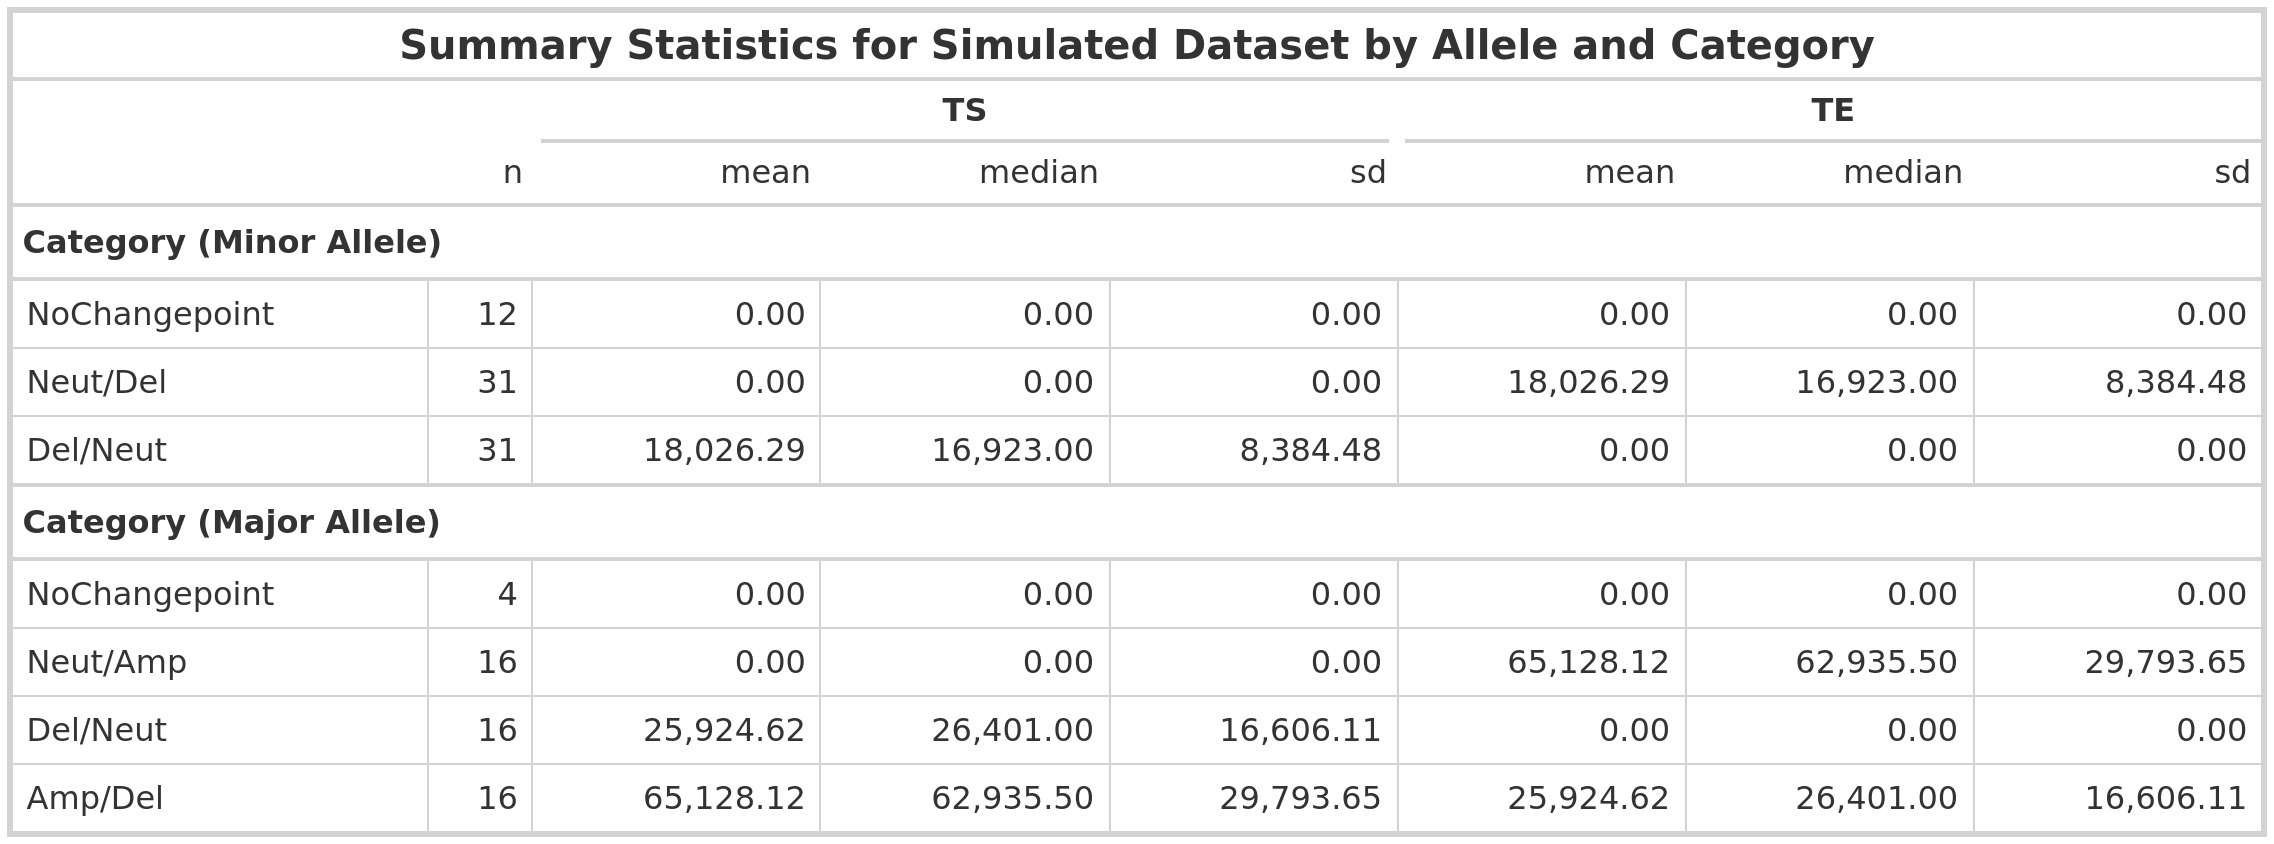
\includegraphics[width = 1\textwidth]{../tables/Chapter_5/Indv_Simulated_Example_Allele_Summary_Table.png}
\label{tab:three_tables_1}
\end{table}

Applying univariate ADIMs, for the two responses $TS$ and $TE$, provides model parameter and interval estimates (Table \ref{tab:lm_uni_AD_modpred} and Figure \ref{fig:lm_uni_AD_modpred}). Table \ref{tab:lm_uni_AD_modpred} shows agreement between the parameter estimates and the mean lengths of the $TS$ and $TE$ recorded in Table \ref{tab:three_tables_1}, across all categories and alleles, indicating that our fitted univariate ADIMs seem to be estimating the parameters as intended. Table \ref{tab:lm_uni_AD_modpred} and Figure \ref{fig:lm_uni_AD_modpred} demonstrate that the mean lengths of $TS$ for the Del/Neut and Amp/Del categories on the Major allele, the mean length of $TS$ for the Del/Neut categories on the Minor allele, the mean lengths of $TE$ for the Neut/Amp and Amp/Del categories on the Major allele and the mean lengths of $TE$ for the Neut/Del categories on the Minor alleles, are all significantly greater than 0. 

\begin{table}[H]
\centering
\caption[Univariate Allele-Dependent Intercept Model parameter estimates and intervals fitted using \texttt{lm()}.]{Univariate Allele-Dependent Intercept parameter estimates and intervals fitted using \texttt{lm()} and where neutral lengths are recorded as 0. Fit, LB and UB correspond to the parameter estimates and associated 95\% confidence intervals. }
      
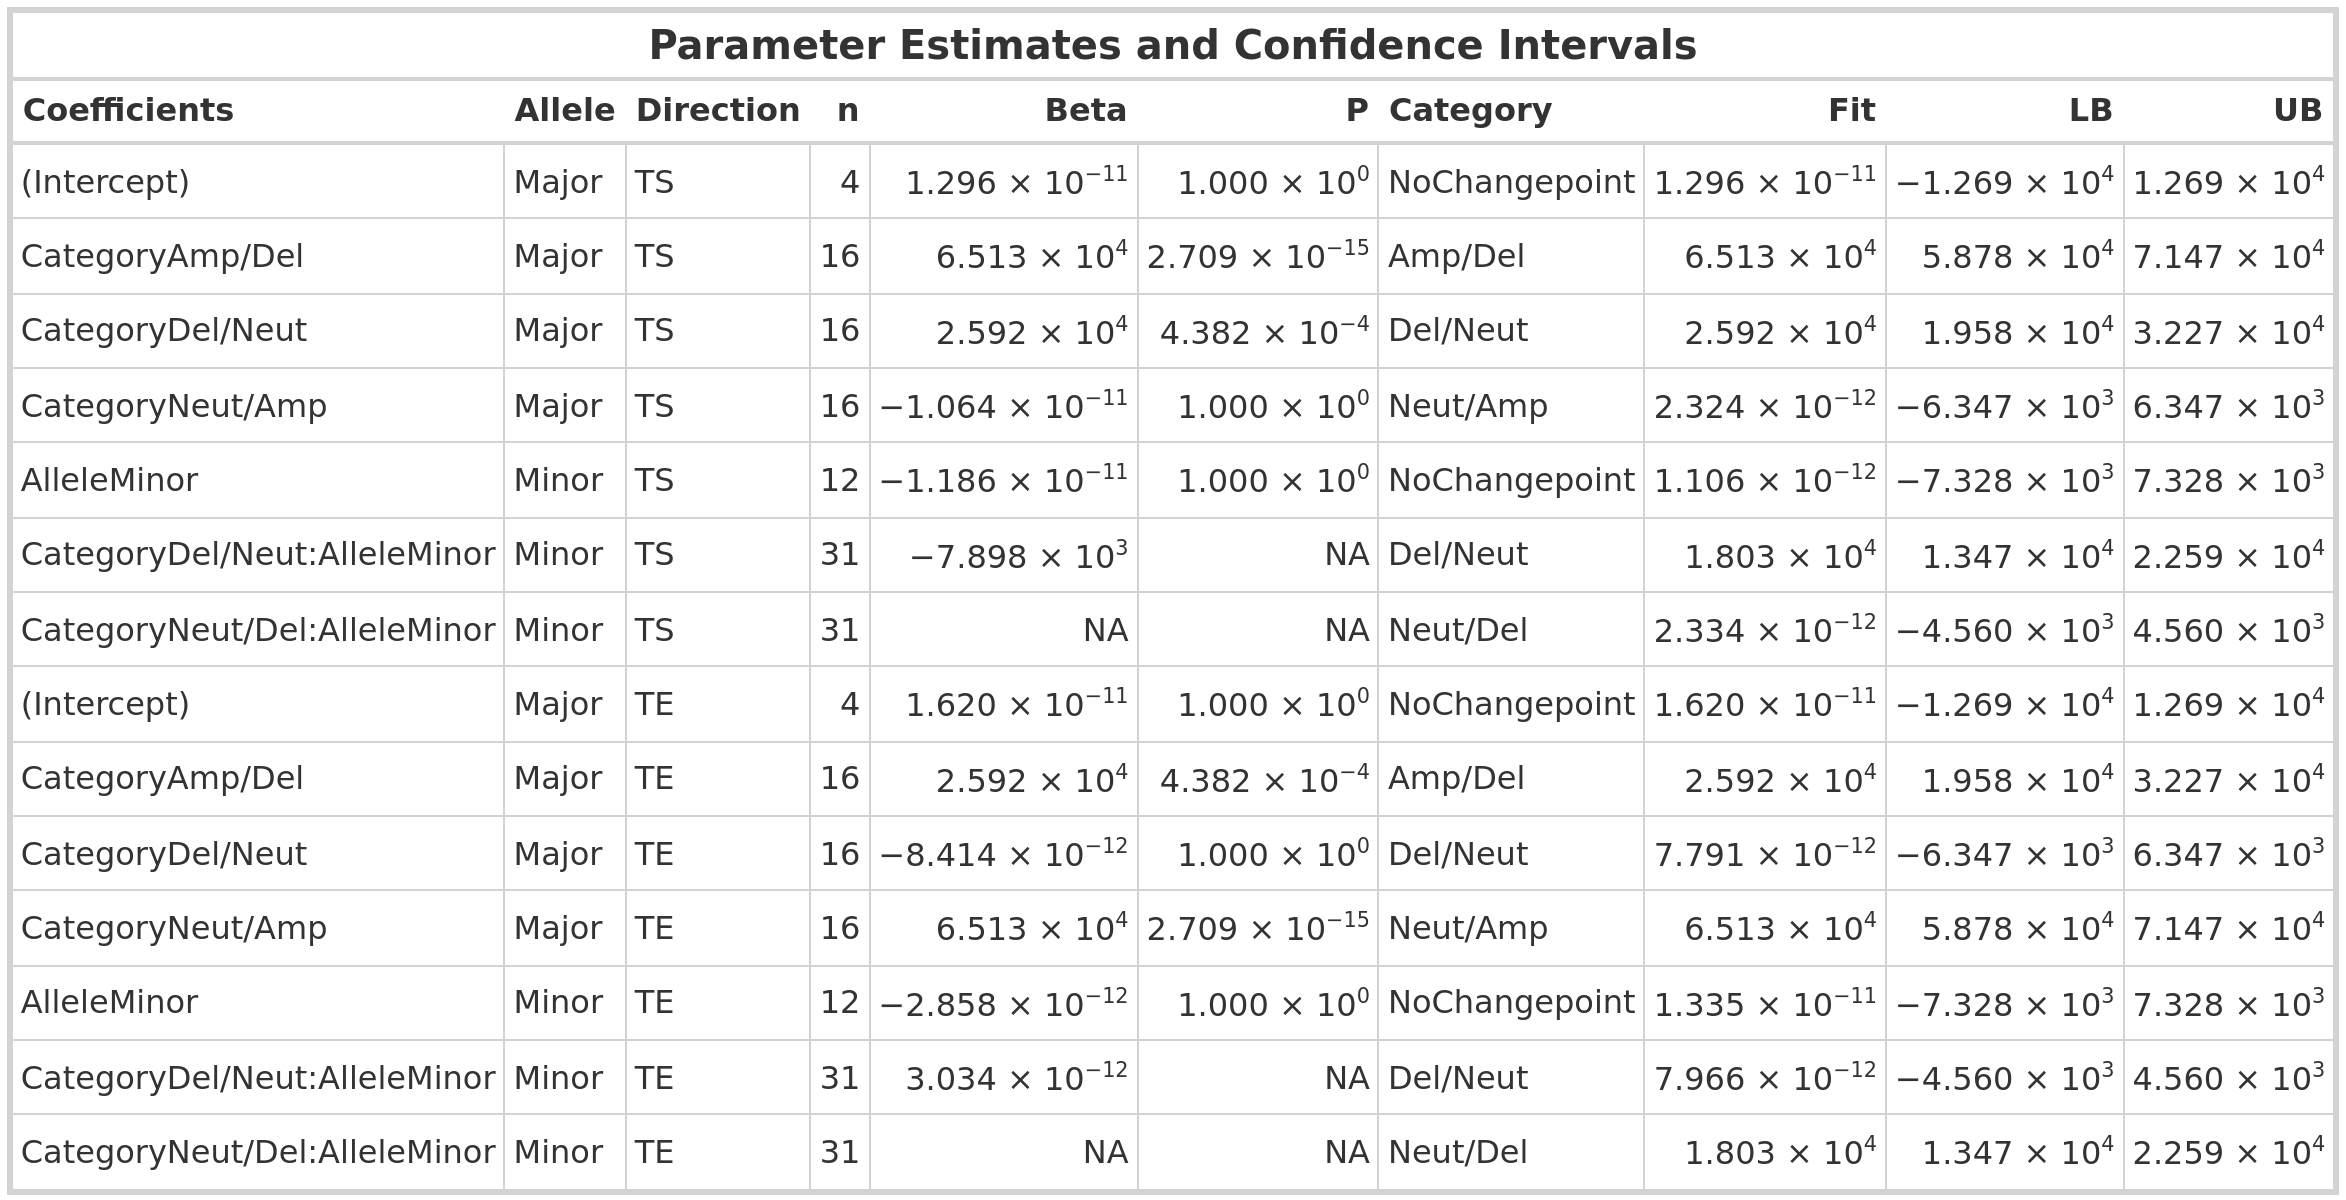
\includegraphics[width = 1\textwidth]{../tables/Chapter_5/Univariate_lm_7_AD_Model_Pred.png}
\label{tab:lm_uni_AD_modpred}
\end{table}

\begin{figure}[H] 
\centering
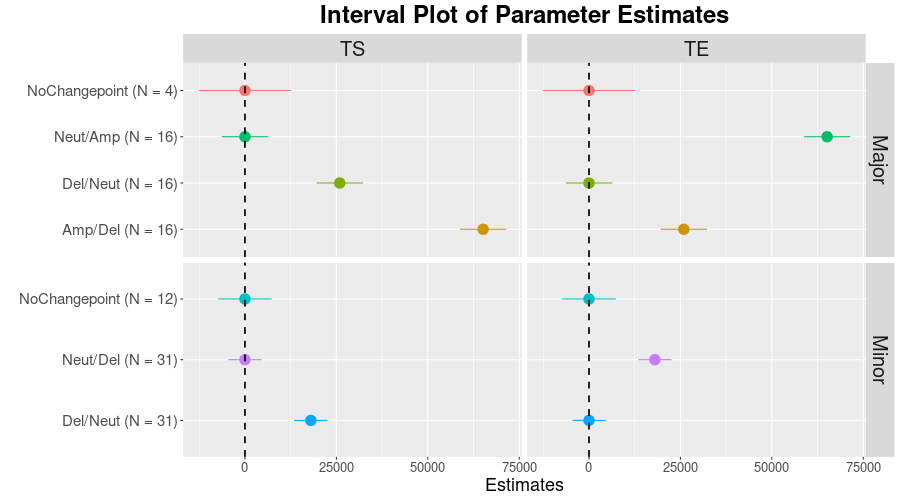
\includegraphics[width = 0.8\textwidth]{../figures/Chapter_5/Univariate_lm_7_AD_Interval.png}
 
\caption[Interval plot of univariate Allele-Dependent Intercept Model parameter estimates fitted using \texttt{lm()}.]{Interval plot of univariate Allele-Dependent Intercept Model parameter estimates fitted using \texttt{lm()} and where neutral lengths are recorded as 0.}
\label{fig:lm_uni_AD_modpred}
\end{figure}

Notably, the average of the parameter point estimate for the $TS$ and $TE$ lengths for each category is equal to the parameter point estimates in our AI models. This is expected as the average $TS$ or $TE$ length for each category should be equal, but the addition of the interaction term differentiates which allele the changepoint is observed on, providing more nuanced information about the average lengths of alterations on each allele. In addition, the AD models can highlight changepoints occurring preferentially on one allele, for example, Figure \ref{fig:lm_uni_AD_modpred} indicates that in this dataset the Neut/Amp changepoints are only observed on the Major allele, a detail not provided in the AI models. 

Applying univariate ADNIMs, for the two responses $TS$ and $TE$, provides model parameter and interval estimates (Table \ref{tab:lm_uni_AD_modpred_6} and Figure \ref{fig:lm_uni_AD_modpred_6}). Again, agreement between the parameter estimates and the mean lengths of the $TS$ and $TE$ recorded in Table \ref{tab:three_tables_1} across all categories and alleles is observed. All categories containing a mean $TS$ or $TE$ length significantly greater than 0 on each allele are detected successfully, with the confidence intervals being slightly wider and less precise, for the ADNIMs compared to the ADIMs.

\vfill 
\begin{table}[H]
\centering
\caption[Univariate Allele-Dependent Non-Intercept Model parameter estimates and intervals fitted using \texttt{lm()}.]{Univariate Allele-Dependent Non-Intercept Model parameter estimates and intervals fitted using \texttt{lm()} and where neutral lengths are recorded as 0. Fit, LB and UB correspond to the parameter estimates and associated 95\% confidence intervals. }
      
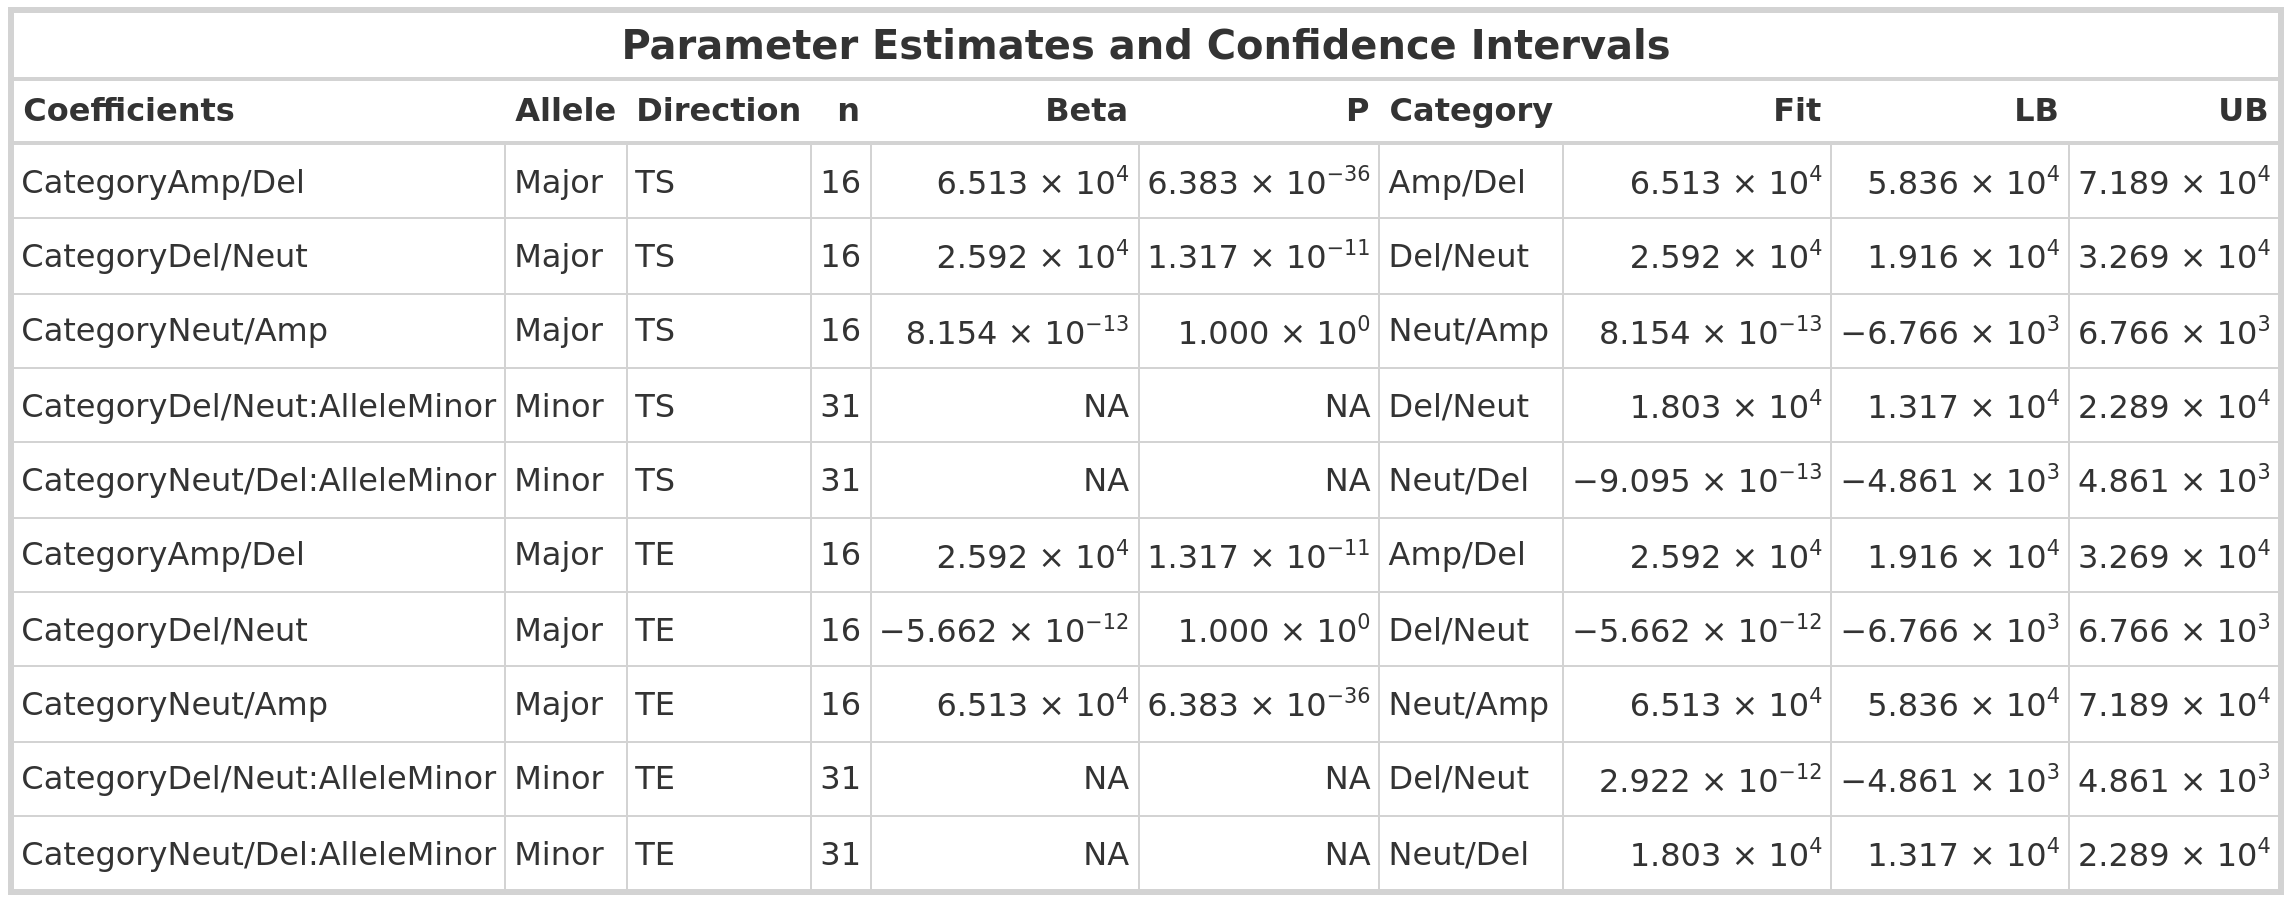
\includegraphics[width = 1\textwidth]{../tables/Chapter_5/Univariate_lm_6_AD_Model_Pred.png}
\label{tab:lm_uni_AD_modpred_6}
\end{table}
\vspace{0.3cm}
\begin{figure}[H] 
\centering
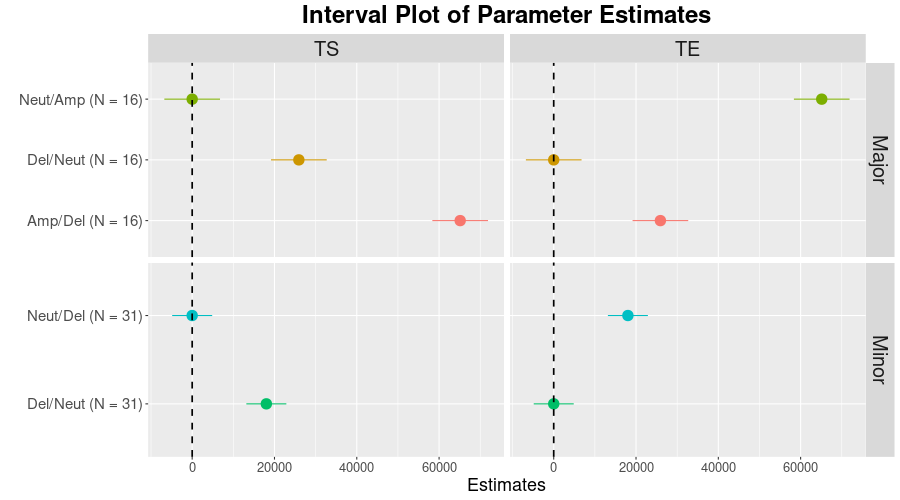
\includegraphics[width = 0.80\textwidth]{../figures/Chapter_5/Univariate_lm_6_AD_Interval.png}
 
\caption[Interval plot of univariate Allele-Dependent Non-Intercept Model parameter estimates fitted using \texttt{lm()}.]{Interval plot of univariate Allele-Dependent Non-Intercept Model parameter estimates fitted using \texttt{lm()} and where neutral lengths are recorded as 0.}
\label{fig:lm_uni_AD_modpred_6}
\end{figure}
\vfill 
\clearpage 

As expected the results of fitting the multivariate ADIM (Table \ref{tab:lm_multi_AD_modpred} and Figure \ref{fig:lm_multi_AD_modpred}) and ADNIM (Table \ref{tab:lm_multi_AD_modpred_6} and Figure \ref{fig:lm_multi_AD_modpred_6}) to the simulated data mirror those obtained from the univariate models, with the exception of the confidence intervals, which are absent in the models fitted using the \texttt{lm()} function. Multivariate ADIM and ADNIM, fitted using the \texttt{MCMCglmm()} function, are provided in Appendix E.

Overall, these models indicate that there is minimal difference in the categories detected using the Intercept and Non-Intercept models. However, due to sample size concerns in datasets where very few changepoints are present, the decision was made to include the NoChangepoint observations. In addition, these AD models provide valuable information regarding which allele the CNA changepoint has occurred on, highlighting instances where changepoint categories occur preferentially on one allele and instances where average lengths of alteration segments, $TS$ and $TE$, may differ between alleles.

\vfill 
\begin{table}[!h]
\centering
\caption[Multivariate Allele-Dependent Intercept Model parameter parameter estimates and intervals fitted using \texttt{lm()}.]{Multivariate Allele-Dependent Intercept Model parameter estimates and intervals fitted using \texttt{lm()} and where neutral lengths are recorded as 0. Fit, LB and UB correspond to the parameter estimates and associated 95\% confidence intervals. }
      
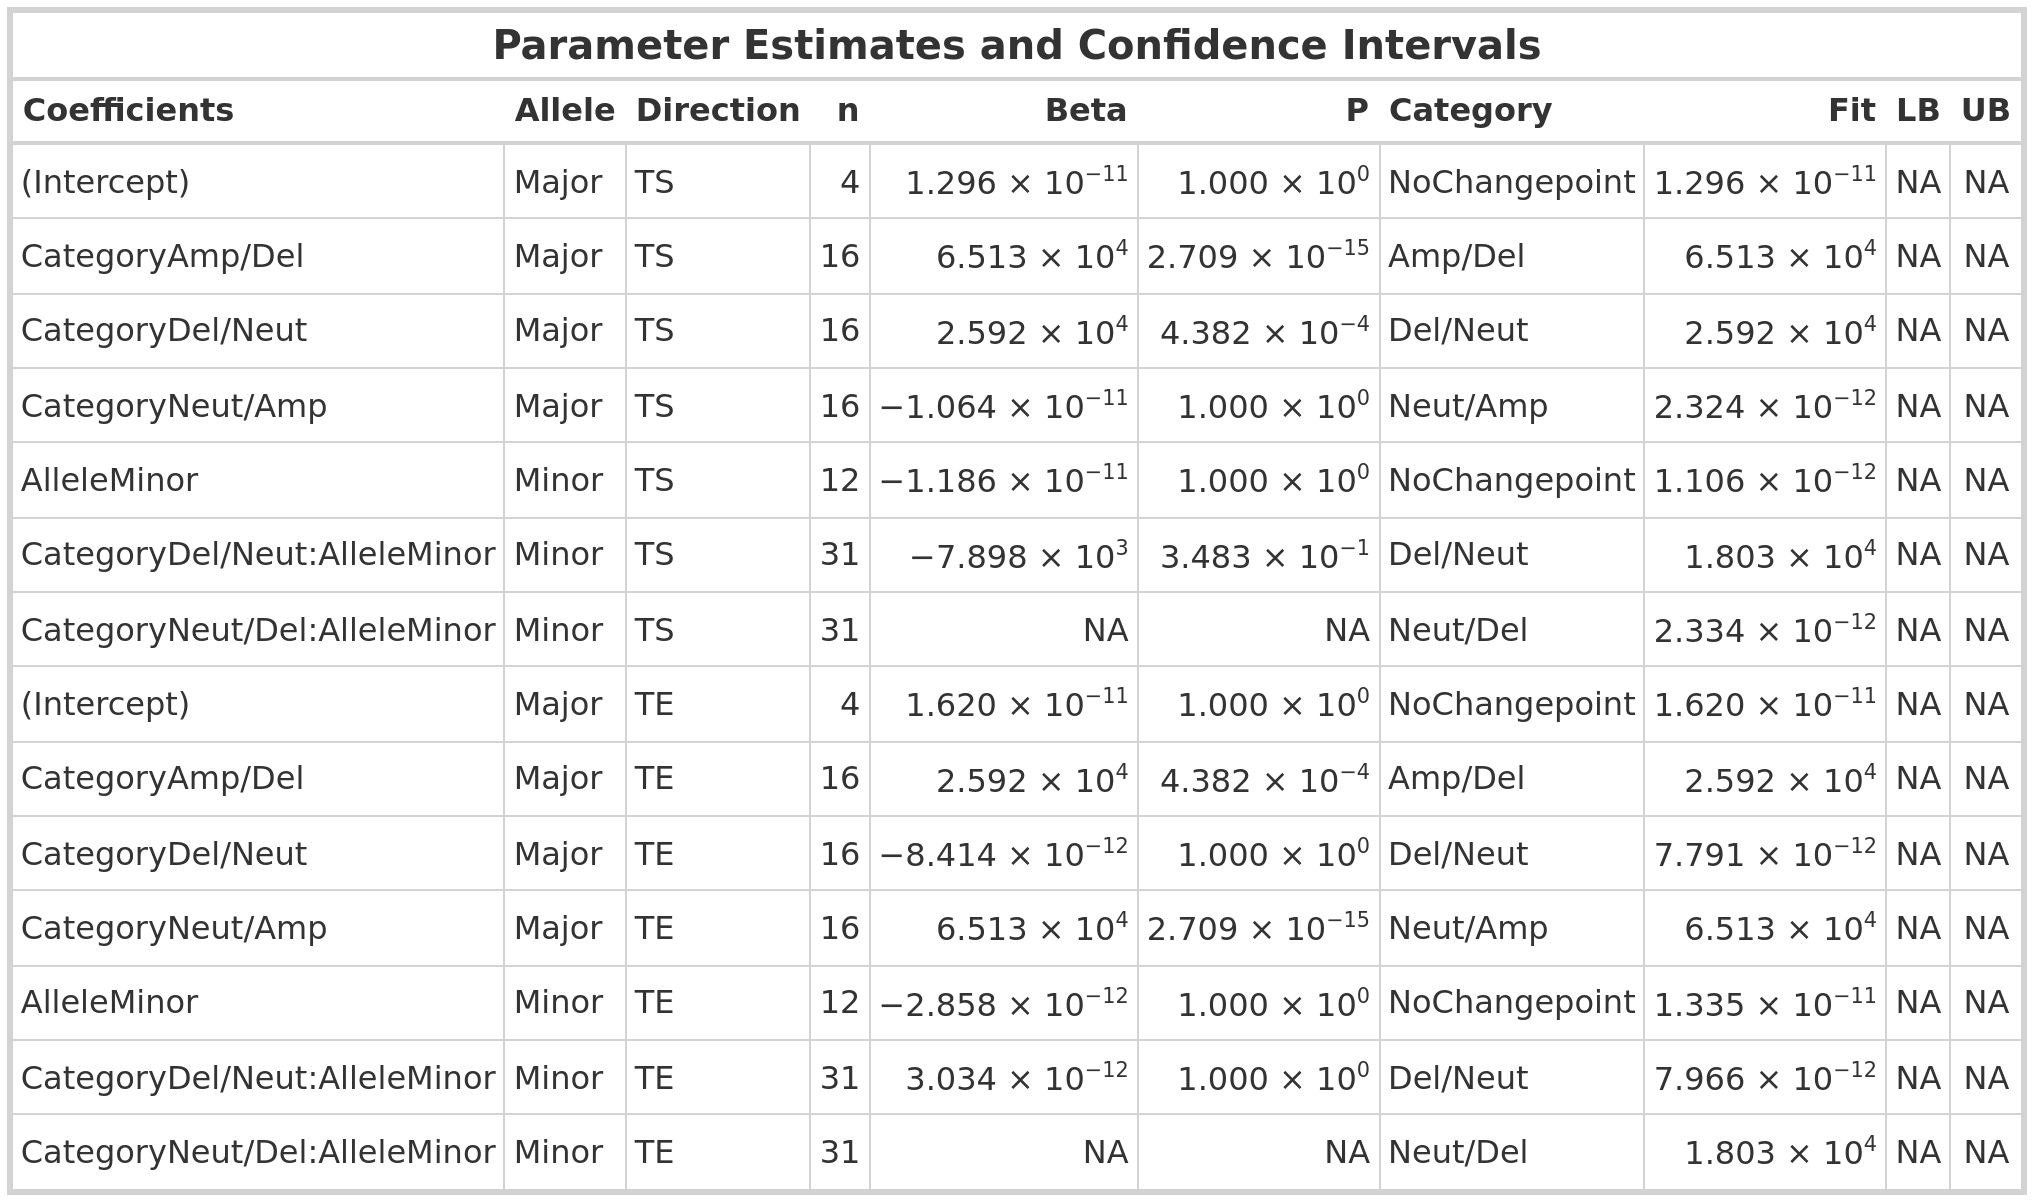
\includegraphics[width = 1\textwidth]{../tables/Chapter_5/Multivariate_lm_7_AD_Model_Pred.png}
\label{tab:lm_multi_AD_modpred}
\end{table}
\vfill 

\begin{figure}[!h]
\centering
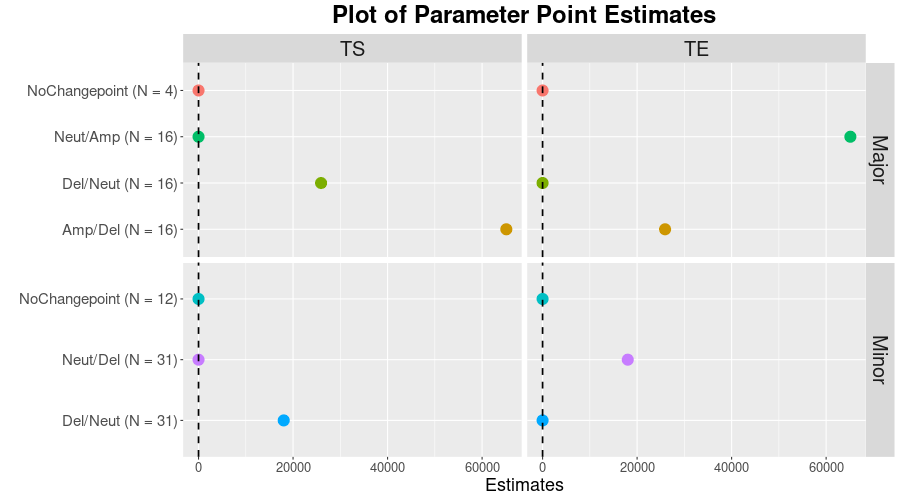
\includegraphics[width = 0.8\textwidth]{../figures/Chapter_5/Multivariate_lm_7_AD_Interval.png}
 
\caption[Plot of multivariate Allele-Dependent Intercept Model parameter estimates fitted using \texttt{lm()}.]{Plot of multivariate Allele-Dependent Intercept Model parameter estimates fitted using \texttt{lm()} and where neutral lengths are recorded as 0.}
\label{fig:lm_multi_AD_modpred}
\end{figure}

\begin{table}[!h]
\centering
\caption[Multivariate Allele-Dependent Non-Intercept Model parameter estimates and intervals fitted using \texttt{lm()}.]{Multivariate Allele-Dependent Non-Intercept Model parameter estimates and intervals fitted using \texttt{lm()} and where neutral lengths are recorded as length 0. Fit, LB and UB correspond to the parameter estimates and associated 95\% confidence intervals.}

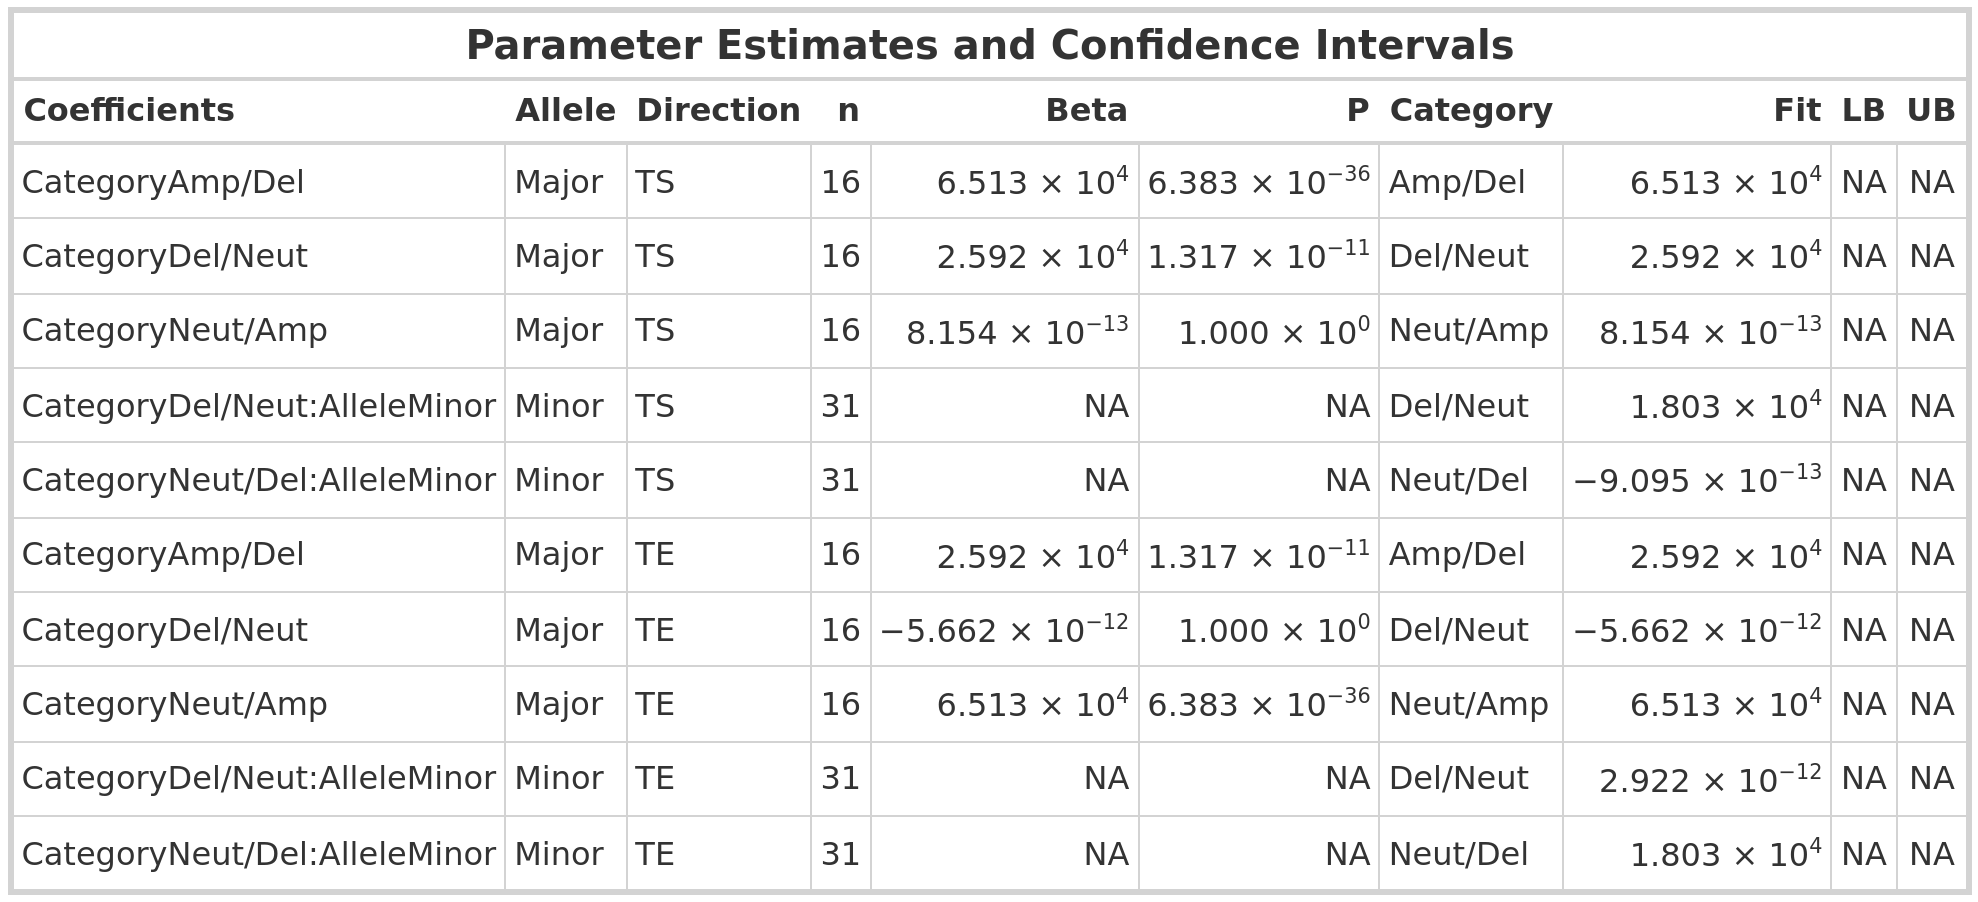
\includegraphics[width = 1\textwidth]{../tables/Chapter_5/Multivariate_lm_6_AD_Model_Pred.png}
\label{tab:lm_multi_AD_modpred_6}
\end{table}
\clearpage

\begin{figure}[H]  
\centering
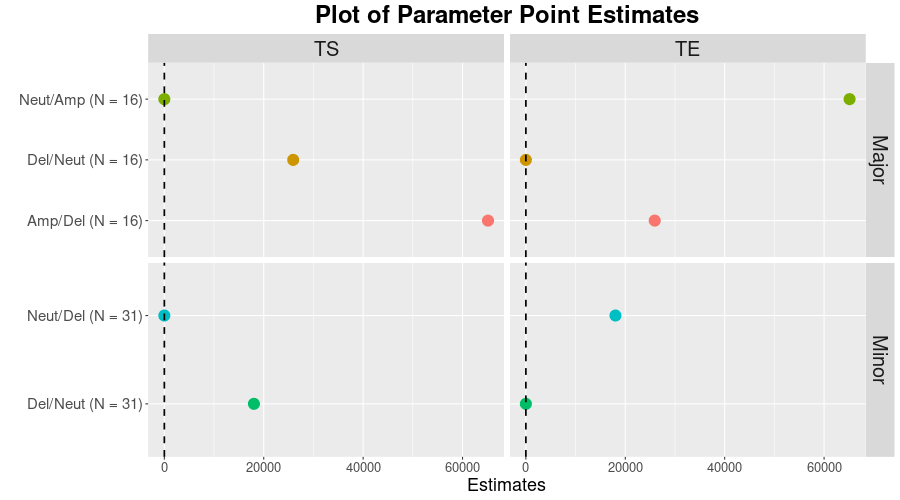
\includegraphics[width = 0.8\textwidth]{../figures/Chapter_5/Multivariate_lm_6_AD_Interval.png}
 
\caption[Plot of multivariate Allele-Dependent Non-Intercept Model parameter estimates fitted using \texttt{lm()}.]{Plot of multivariate Allele-Dependent Non-Intercept Model parameter estimates fitted using \texttt{lm()} and where neutral lengths are recorded as 0.}
\label{fig:lm_multi_AD_modpred_6}
\end{figure} 

\subsection{Simulation Study}
To explore the behaviour of the proposed AD models, a variety of scenarios are simulated, with varying sample sizes and profile compositions.
\newline

Scenario 1 assigns:
\begin{itemize}
\item a percentage of samples to have one of the two alleles displaying an amplified segment within the observed region (CNA profile B), and 
\item a percentage of samples to  have no CNAs, i.e. no changepoints, in the observed region, for both alleles (CNA profile A). 
\end{itemize}

Scenario 2 assigns:
\begin{itemize}
\item a percentage of samples to have one of the two alleles displaying an amplified segment followed by a deleted segment (what we define as an Amp/Del flashpoint pattern) within the observed region (CNA profile C), and 
\item a percentage of samples to have one of the two alleles displaying an amplified segment within the observed region (CNA profile B).
\end{itemize}

Scenario 3 assigns:
\begin{itemize}
\item a percentage of samples to have allele-specific copy number profile D, where one allele displays an Amp/Del flashpoint pattern flanked by two neutral segments and the other allele displays an oscillating pattern of deleted and neutral segments,
\item a percentage of samples to have one of the two alleles displaying an amplified segment followed by a deleted segment (Amp/Del flashpoint pattern), within the observed region (CNA profile C), and 
\item a percentage of samples to have no CNAs, i.e. no changepoints, in the observed region, for both alleles (CNA profile A). 
\end{itemize}

In setting parameters to generate the profiles, we assume a region similar in length to chromosome 1 ($\approx 250,000$kb) as the genomic region. Lengths are generated from truncated Normal distributions, mean lengths of CNA segments are similar to those observed in the ASCAT data (Tables \ref{tbl:excel-table1} and \ref{tbl:excel-table2}), as specified in Table \ref{tab:Param}.

\begin{table}[!htb]
\vspace{0.5cm}
\center
\caption[Parameters of truncated Normal distributions used to simulate segment lengths and properties of simulated scenarios.]{Parameters of truncated Normal distributions used to simulate segment lengths and properties of simulated scenarios. a and b correspond to the lower and upper bound.}
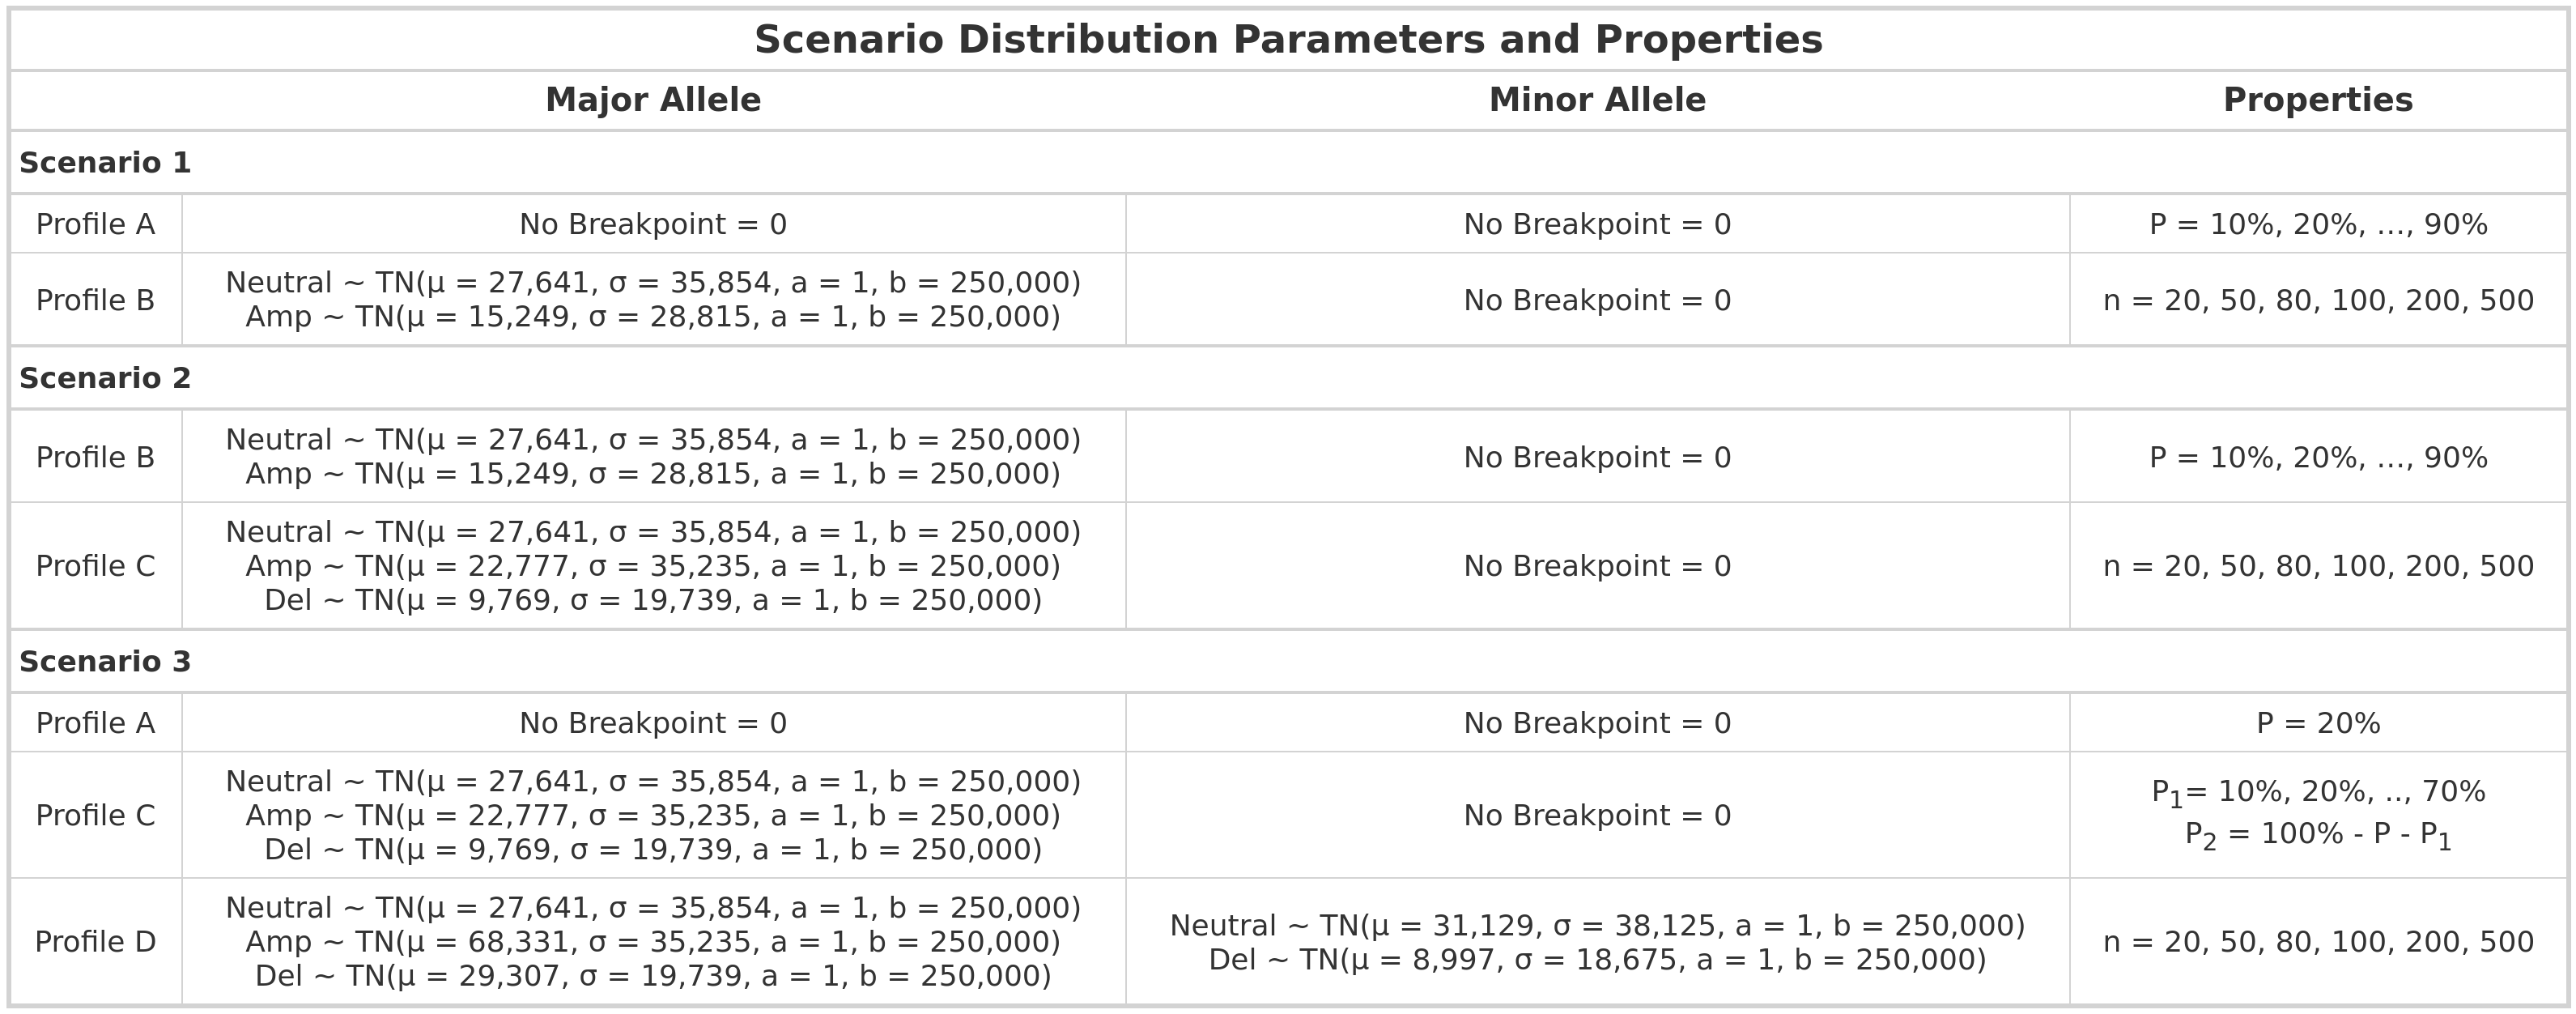
\includegraphics[width = 1\textwidth]{../tables/Chapter_5/TN_Distribution.png}
\label{tab:Param}
\end{table}

For scenario 1, datasets are generated varying the size of the dataset, n, ranging from 20 to 500, and varying the percentage of the dataset having a CNA, $P$, ranging from 20\% to 90\% of samples displaying allele-specific copy number profile B. For each specification, 20 replicated datasets were simulated. Scenario 2 consists of allele-specific copy number profiles B and C, at varying percentages $P$ and $1-P$, each with 20 replications. For scenario 3, three possible allele-specific copy number profiles, A, C and D, setting the percentage of samples displaying profile A at $P = 20\%$ and with varying percentages of samples displaying allele-specific copy number profile C and D, $P_1$ and $P_2$, each with 20 replications, are generated. In all datasets the lengths of the neutral segments are recorded as length 0 and the NoChangepoint category is retained. 

Univariate and multivariate AD models (ADIM) are fitted to all simulated datasets and assessed. An illustration of the distribution of point estimates across the replicated datasets, for example in simulated scenario 1, is provided in Figures \ref{fig:DP_1}-\ref{fig:DP_2}. The $TS$ and $TE$ point estimates for each category and allele, over the 20 replications, indicate the variability in simulated datasets and that lengths simulated as 0 are observed to have points estimates around 0.

\begin{figure}[!ht]
\vspace{0.5cm}
     \begin{subfigure}[t]{.49\textwidth}
      \centering
     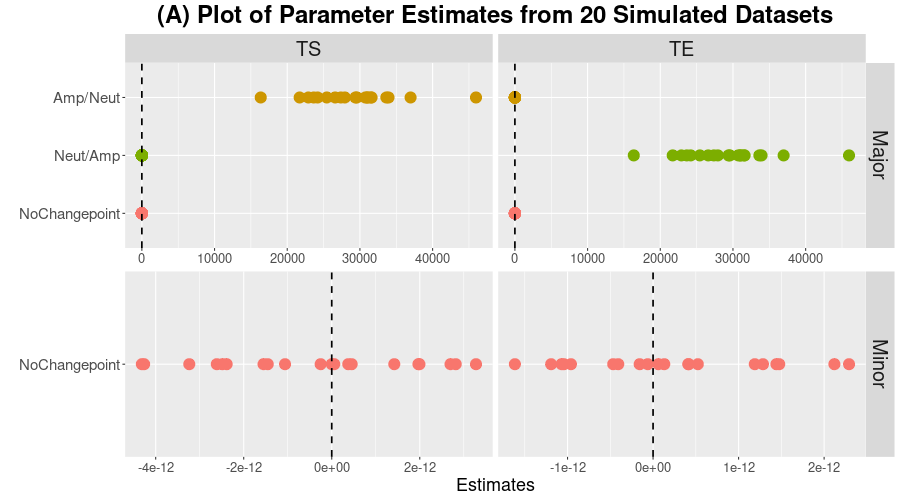
\includegraphics[width = 1\textwidth]{../figures/Chapter_5/Uni_lm_Prediction_Simulation.png}
    \end{subfigure}%
     \begin{subfigure}[t]{.49\textwidth}
      \centering
       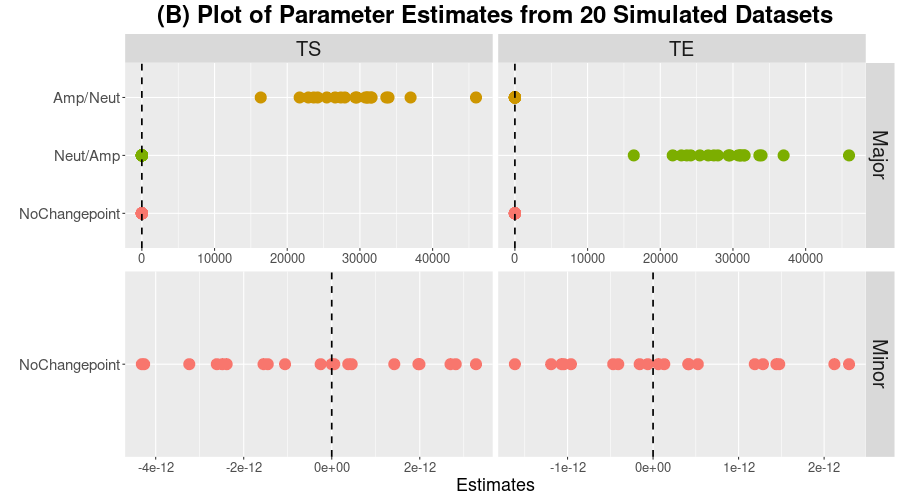
\includegraphics[width = 1\textwidth]{../figures/Chapter_5/Uni_MCMC_Prediction_Simulation.png}
    \end{subfigure} 
     \caption[Plot of univariate Allele-Dependent Intercept Model parameter estimates for simulated scenario 1 with $n = 50$ and $P = 20$.]{Plot of univariate Allele-Dependent Intercept Model parameter estimates for simulated scenario 1 with $n = 50$ and $P = 20$ fitted using the (A) \texttt{lm()} function and (B) \texttt{MCMCglmm()} function. Scales on the x-axis vary between alleles.}
     \label{fig:DP_1}
\end{figure}

\begin{figure}[!ht]
\vspace{0.5cm}
     \begin{subfigure}[t]{.49\textwidth}
      \centering
     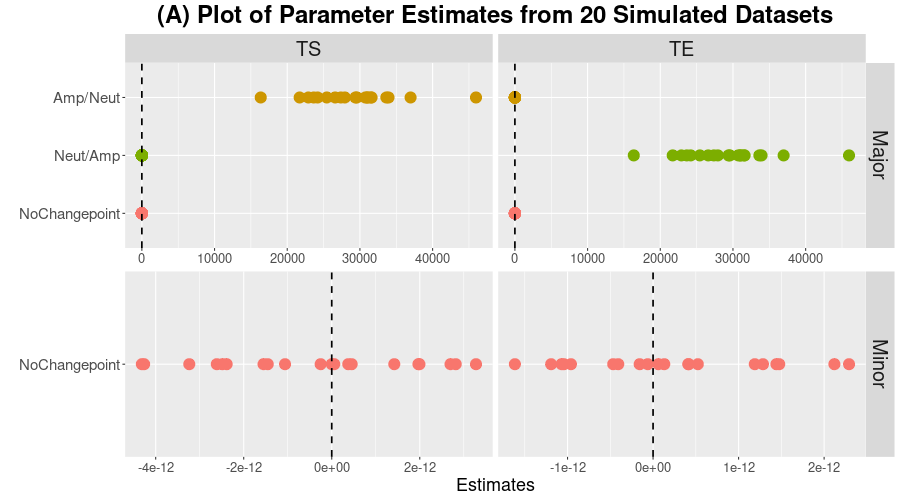
\includegraphics[width = 1\textwidth]{../figures/Chapter_5/Multi_lm_Prediction_Simulation.png}
    \end{subfigure}%
     \begin{subfigure}[t]{.49\textwidth}
      \centering
       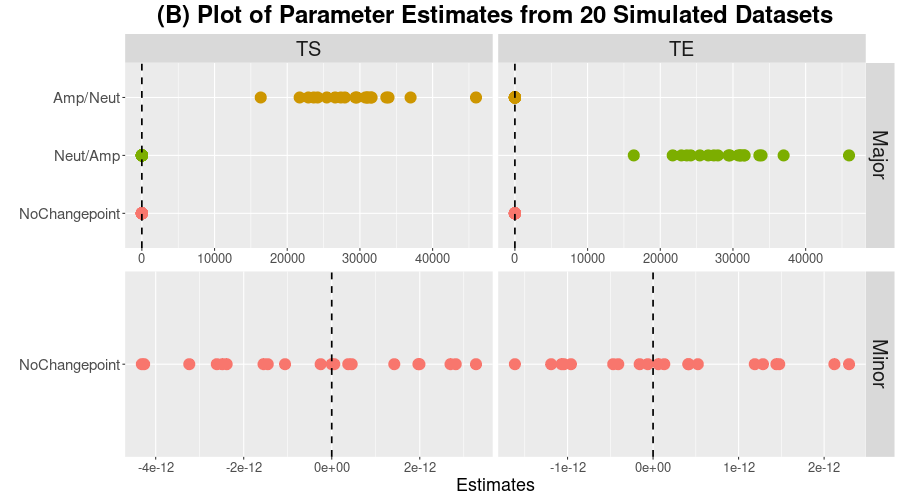
\includegraphics[width = 1\textwidth]{../figures/Chapter_5/Multi_MCMC_Prediction_Simulation.png}
    \end{subfigure} 
     \caption[Plot of multivariate Allele-Dependent Intercept Model parameter estimates for simulated scenario 1 with $n = 50$ and $P = 20$.]{Plot of multivariate Allele-Dependent Intercept Model parameter estimates for simulated scenario 1 with $n = 50$ and $P = 20$ fitted using the (A) \texttt{lm()} function and (B) \texttt{MCMCglmm()} function. Scales on the x-axis vary between alleles.}
     \label{fig:DP_2}
\end{figure}

The significance of a changepoint category is assessed based on the confidence interval of the parameter being strictly positive, i.e. the value of the lower bound of the interval, $LB > 0$. The proportion of datasets observed to indicate significance of that parameter when fitted with univariate \texttt{lm()} and univariate \texttt{MCMCglmm()} are provided in Figure \ref{fig:Uni_lm_SimStudy} and Figure \ref{fig:Uni_mcmc_SimStudy}, respectively. For scenario 1, the categories with simulated $TS$ length, Amp/Neut, and $TE$ length, Neut/Amp, are detected consistently on the Major allele across all simulated sample sizes and profile percentages. For scenario 2, with more categories and complex structure, more variability is observed but as the sample size increases the effect of this variability decreases and the types of changepoints simulated in the scenario are detected as significant. Similarly for the complexity of scenario 3, the $TS$ Amp/Del and Del/Neut and $TE$ Amp/Del and Neut/Amp on the Major allele, and the $TS$ Del/Neut and $TE$ Neut/Del on the Minor allele, are consistently detected across all sample sizes and profile percentages. 

Fits produced from the multivariate AD models, using the \texttt{MCMCglmm()} function produces similar results to the univariate models and shows that as the sample size increases, the types of changepoints simulated in the scenario are detected as significant (Figure \ref{fig:Multi_mcmc_SimStudy}).

In the univariate and multivariate MCMCglmm fit of ADIM, we observe decreased True Positive rate for smaller sample sizes, evident in particular for scenario 2. Taking a closer look at individual datasets in scenario 2 reveals that for sample size $n = 20$, where 90\% of samples display copy number profile C, the Amp/Neut category occurs only twice and as such the $TS$ is not detected in approximately 35\% of datasets (Table \ref{tbl:Individual_1}). In addition, where 10\% of samples display copy number profile C, the Amp/Del category appears only twice and the $TE$ is not detected in approximately 55\% of datasets (Table \ref{tbl:Individual_1}). This indicates that the variability is due to the small sample size and decreased profile percentages of those specific categories. 

Overall, it appears that for the majority of categories and scenarios, as the profile percentage or sample size increases, the detection of each category simulated goes to 1. Notably, by using intervals to assess significance, we can also identify regions where changepoints over a certain length occur, i.e. over $1,000$kb. This is done by checking whether the lower bound of the confidence interval is greater than 1,000 ($LB > 1000$).

\vfill 
\begin{figure}[!htb]
\center
\includegraphics[width = 1\textwidth]{../figures/Chapter_5/lm_uni_sim_plot.png}
\caption[Plot displaying the proportion of the 20 simulated datasets, for each sample size and percentage, where the category was detected by our proposed univariate Allele-Dependent Intercept Model (\texttt{lm()}).]{Plot displaying the proportion of the 20 simulated datasets, for each sample size and percentage, where the category was detected by our proposed univariate Allele-Dependent Intercept Model. Fitted using the \texttt{lm()} function. Significance of a changepoint category assessed using $LB > 0$.}
\label{fig:Uni_lm_SimStudy}
\end{figure}

\begin{figure}[!htb]
\center
\includegraphics[width = 1\textwidth]{../figures/Chapter_5/MCMC_uni_sim_plot.png}
\caption[Plot displaying the proportion of the 20 simulated datasets, for each sample size and percentage, where the category was detected by our proposed univariate Allele-Dependent Intercept Model (\texttt{MCMCglmm()}).]{Plot displaying the proportion of the 20 simulated datasets, for each sample size and percentage, where the category was detected by our proposed univariate Allele-Dependent Intercept Model. Fitted using the \texttt{MCMCglmm()} function. Significance of a changepoint category assessed using $LB > 0$.}
\label{fig:Uni_mcmc_SimStudy}
\end{figure}
\vfill 

\clearpage

\begin{figure}[!htb]
\vspace{1.6cm}
\center
\includegraphics[width = 1\textwidth]{../figures/Chapter_5/MCMC_multi_sim_plot.png}
\caption[Plot displaying the proportion of the 20 simulated datasets, for each sample size and percentage, where the category was detected by our proposed multivariate Allele-Dependent Intercept Model (\texttt{MCMCglmm()}).]{Plot displaying the proportion of the 20 simulated datasets, for each sample size and percentage, where the category was detected by our proposed multivariate Allele-Dependent Intercept Model. Fitted using the \texttt{MCMCglmm()} function. Significance of a changepoint category assessed using $LB > 0$.}
\label{fig:Multi_mcmc_SimStudy}
\end{figure}

\begin{table}[!h]
  \caption[Parameter estimates for selected Allele-Dependent Intercept Model MCMCglmm fits.]{Parameter estimates for selected Allele-Dependent Intercept Model MCMCglmm fits. (A) $TS$ Amp/Neut category and (B) $TE$ Amp/Del category, where $n = 20$, across 20 simulated datasets. Fit, LB and UB correspond to the parameter estimates and associated 95\% confidence intervals.}
  \label{tbl:Individual_1}
  \includegraphics[width=0.5\linewidth]{"../tables/Chapter_5/Model_Scenario_2_Closer_Look_1.png"}
  \includegraphics[width=0.5\linewidth]{"../tables/Chapter_5/Model_Scenario_2_Closer_Look_2.png"}
\end{table}

\subsection{Conclusions}
Allele-specific copy number profiling provides information on genome wide copy number for each allele and tackles some of the limitations of total copy number profiling, including masking of changepoints and certain types of genomic aberrations. 

To use allele-specific copy number profiles, produced using ASCAT, to identify and characterise copy number associated changepoints based on the lengths of the flanking alteration segments, $TS$ and $TE$, AD models, ADIM and ADNIM are proposed, including interaction terms, to detect the presence of these changepoints and their performance assessed across a number of scenarios. 

It was observed that AI and AD models performed as expected when applying them to simulated datasets, where consideration was given to the form of data the models are applied to, including recording neutral segment length and retention of the NoChangepoint category. It was noted that while the confidence intervals were wider in cases where the neutral segments were retained as lengths greater than 0, and also in cases where the NoChangepoint category was excluded, the simulated categories are significantly greater than 0 in all cases and the overall conclusions the same. As our focus is on flanking alteration segments, the decision was made to record neutral segment lengths as 0, and due to sample size concerns, the decision was made to include NoChangepoint observations.

The AI and AD models perform similarly, estimating the mean lengths of $TS$ and/or $TE$ for the simulated categories as significantly greater than 0. Importantly, the AD models provide more detailed information regarding which allele the changepoint has occurred on, enabling identification of cases where a changepoint category occurs preferentially on one allele and cases where the average lengths of alteration segments may differ between alleles. 

Assessing how the AD models, fitted using the \texttt{lm()} and \texttt{MCMCglmm()} functions, perform across datasets of varying sample sizes and profile percentages, indicates that the univariate ADIM, fitted using the \texttt{lm()} and \texttt{MCMCglmm()} functions, and the multivariate ADIM, fitted using the \texttt{MCMCglmm()} function, performed consistently well across sample sizes and profile percentages. The multivariate AD models, fitted using the \texttt{lm()} function, were lacking confidence intervals, a result of limitations in the software.

In the next chapter the selected models, univariate ADIM fitted using \texttt{lm()} and multivariate ADIM fitted using \texttt{MCMCglmm()}, will be applied to the allele-specific copy number profiles generated for the METABRIC data. In this application, the observed interval $d$ is either a gene region, i.e. between the start and end position of a gene, or segments of the genome, generated using a segmentation or sliding window approach. The resulting significant regions will then be analysed, identifying regions of the genome where allele-specific changepoints occur and further investigation is warranted. 